\documentclass[12pt]{article}

%Paquetes
\usepackage{titlesec}
\usepackage[dvipsnames]{xcolor}
\usepackage{lipsum}
\usepackage{fontspec}
\usepackage{graphicx} %Imágenes
\usepackage{colortbl}
\usepackage{setspace}
\usepackage[a4paper]{geometry}
\usepackage{fancyhdr}
\usepackage[babel]{csquotes}
\usepackage[spanish, english]{babel}
\usepackage{apacite} % Norma APA bibliografía
\usepackage{natbib} %Bibliografía
\usepackage[nottoc]{tocbibind}
\usepackage[acronym,nonumberlist,toc]{glossaries} % Configuraciones glosario
\usepackage{glossary-superragged} %Configuraciones glosario
\usepackage[hang,flushmargin]{footmisc}
\usepackage{etoolbox}
\usepackage[hidelinks, breaklinks=true]{hyperref}
\usepackage{booktabs} % Tablas
\usepackage{tabularx}
\usepackage{float}
\usepackage{hyperref}
\usepackage{nameref}
\usepackage{verbatim} % Para comentarios multilinea
\usepackage{longtable} % tablas grandes
\usepackage{listings}
\usepackage{color}
\usepackage{fontawesome5} % Iconos de FontAwesome
\usepackage{caption}
\usepackage{subcaption}
\usepackage{tikz} % diagramas
\usetikzlibrary{arrows.meta, positioning}
\usepackage{rotating} % para rotar tablas
\usepackage{makecell}
\usepackage{pdflscape} % rotar páginas
\usepackage{amsmath}
\usepackage{amsfonts}

\definecolor{myred}{HTML}{E74C3C}
\definecolor{mygreen}{HTML}{27AE60}

\definecolor{dkgreen}{RGB}{0,0.6,0}
\definecolor{gray}{RGB}{0.5,0.5,0.5}
\definecolor{mauve}{RGB}{0.58,0,0.82}
\definecolor{delim}{RGB}{20,105,176}
\definecolor{numb}{RGB}{106, 109, 32}
\definecolor{string}{RGB}{0.64,0.08,0.08}

%%%%%%%%%%%%%%%%%%%%%%%%%%%%%%%%%%%%%%%%%%%%%%%%%%%%%%
%%%%%%%%%%% YAML syntax highlighting %%%%%%%%%%%%%%%%%

% http://tex.stackexchange.com/questions/152829/how-can-i-highlight-yaml-code-in-a-pretty-way-with-listings

% here is a macro expanding to the name of the language
% (handy if you decide to change it further down the road)
\newcommand\YAMLcolonstyle{\color{red}\mdseries}
\newcommand\YAMLkeystyle{\color{black}\bfseries}
\newcommand\YAMLvaluestyle{\color{blue}\mdseries}

\makeatletter

\newcommand\language@yaml{yaml}

\expandafter\expandafter\expandafter\lstdefinelanguage
\expandafter{\language@yaml}
{
	keywords={true,false,null,y,n},
	keywordstyle=\color{darkgray}\bfseries,
	basicstyle=\YAMLkeystyle,                                 % assuming a key comes first
	sensitive=false,
	comment=[l]{\#},
	morecomment=[s]{/*}{*/},
	commentstyle=\color{purple}\ttfamily,
	stringstyle=\YAMLvaluestyle\ttfamily,
	moredelim=[l][\color{orange}]{\&},
	moredelim=[l][\color{magenta}]{*},
	moredelim=**[il][\YAMLcolonstyle{:}\YAMLvaluestyle]{:},   % switch to value style at :
	morestring=[b]',
	morestring=[b]",
	literate =    {---}{{\ProcessThreeDashes}}3
	{>}{{\textcolor{red}\textgreater}}1     
	{|}{{\textcolor{red}\textbar}}1 
	{\ -\ }{{\mdseries\ -\ }}3,
}

% switch to key style at EOL
\lst@AddToHook{EveryLine}{\ifx\lst@language\language@yaml\YAMLkeystyle\fi}
\makeatother

\newcommand\ProcessThreeDashes{\llap{\color{cyan}\mdseries-{-}-}}

%%%%%%%%%%% YAML syntax highlighting %%%%%%%%%%%%%%%%%
%%%%%%%%%%%%%%%%%%%%%%%%%%%%%%%%%%%%%%%%%%%%%%%%%%%%%%

% Python language definition
\lstset{frame=tb,
	language=Python,
	aboveskip=3mm,
	belowskip=3mm,
	showstringspaces=false,
	columns=flexible,
	basicstyle={\small\ttfamily},
	numbers=none,
	numberstyle=\tiny\color{gray},
	keywordstyle=\color{blue},
	commentstyle=\color{dkgreen},
	stringstyle=\color{mauve},
	breaklines=true,
	breakatwhitespace=true,
	tabsize=3
}

% Kotlin language definition
\lstdefinelanguage{Kotlin}{
	comment=[l]{//},
	commentstyle={\color{gray}\ttfamily},
	emph={filter, first, firstOrNull, forEach, lazy, map, mapNotNull, println},
	emphstyle={\color{OrangeRed}},
	identifierstyle=\color{black},
	keywords={!in, !is, abstract, actual, annotation, as, as?, break, by, catch, class, companion, const, constructor, continue, crossinline, data, delegate, do, dynamic, else, enum, expect, external, false, field, file, final, finally, for, fun, get, if, import, in, infix, init, inline, inner, interface, internal, is, lateinit, noinline, null, object, open, operator, out, override, package, param, private, property, protected, public, receiver, reified, return, return@, sealed, set, setparam, super, suspend, tailrec, this, throw, true, try, typealias, typeof, val, var, vararg, when, where, while},
	keywordstyle={\color{NavyBlue}\bfseries},
	escapeinside={//(`}{`)},
	morecomment=[s]{/*}{*/},
	morestring=[b]",
	morestring=[s]{"""*}{*"""},
	ndkeywords={@Composable, @Preview, @Deprecated, @JvmField, @JvmName, @JvmOverloads, @JvmStatic, @JvmSynthetic, Array, Byte, Double, Float, Int, Integer, Iterable, Long, Runnable, Short, String, Any, Unit, Nothing},
	ndkeywordstyle={\color{BurntOrange}\bfseries},
	sensitive=true,
	stringstyle={\color{ForestGreen}\ttfamily},
}

% JSON definition

\lstdefinelanguage{json}{
	numbers=left,
	numberstyle=\small,
	frame=single,
	rulecolor=\color{black},
	showspaces=false,
	showtabs=false,
	breaklines=true,
	postbreak=\raisebox{0ex}[0ex][0ex]{\ensuremath{\color{gray}\hookrightarrow\space}},
	breakatwhitespace=true,
	basicstyle=\ttfamily\small,
	upquote=true,
	morestring=[b]",
	stringstyle=\color{string},
	literate=
	*{0}{{{\color{numb}0}}}{1}
	{1}{{{\color{numb}1}}}{1}
	{2}{{{\color{numb}2}}}{1}
	{3}{{{\color{numb}3}}}{1}
	{4}{{{\color{numb}4}}}{1}
	{5}{{{\color{numb}5}}}{1}
	{6}{{{\color{numb}6}}}{1}
	{7}{{{\color{numb}7}}}{1}
	{8}{{{\color{numb}8}}}{1}
	{9}{{{\color{numb}9}}}{1}
	{\{}{{{\color{delim}{\{}}}}{1}
	{\}}{{{\color{delim}{\}}}}}{1}
	{[}{{{\color{delim}{[}}}}{1}
	{]}{{{\color{delim}{]}}}}{1},
}

%Variables
\definecolor{gray80}{gray}{.80}
\definecolor{blueUnir}{HTML}{0098CD}

\geometry{top=2.5cm, bottom=2.5cm, left=3.0cm, right=2.0cm}
\setmainfont{Calibri}
\spacing{1.5} %Interlineado fijo
\setlength{\parskip}{6pt} %6 puntos de espaciado entre párrafos
\setlength{\parindent}{0cm} %Eliminar sangría
\setlength{\footnotesep}{0pt} %Espaciado entre notas
\setlength{\skip\footins}{1.5cm} %Espaciado entre raya y texto
\renewcommand{\footnotelayout}{\small\baselineskip=10pt} % Interlineado sencillo

\fancyhf{}
\pagestyle{fancy}
\rhead[\fontsize{10pt}{12pt}\setmainfont{Calibri Light}\selectfont Jon Inazio Sánchez Martínez\\Predicción de tráfico mediante aprendizaje profundo y Transformers]{\fontsize{10pt}{12pt}\setmainfont{Calibri Light}\selectfont Jon Inazio Sánchez Martínez\\Predicción de tráfico mediante aprendizaje profundo y Transformers} 
\renewcommand{\headrulewidth}{0pt}
%\renewcommand{\footrulewidth}{1pt}
\rfoot[]{\thepage}
\setcounter{tocdepth}{3} 
\setcounter{secnumdepth}{5}
\newcommand\fh{\babelhyphen{hard}}

\titleformat*{\section}{\fontsize{18pt}{18}\selectfont\color{blueUnir}\setmainfont{Calibri Light}} 
\titleformat*{\subsection}{\fontsize{14pt}{14}\selectfont\color{blueUnir}\setmainfont{Calibri Light}} 
\titleformat*{\subsubsection}{\fontsize{12pt}{12}\selectfont\setmainfont{Calibri}\bfseries}

%
% Acrónimos
%
% La forma de definir un acrónimo es la siguiente:
% \newacronym{id}{siglas}{descripción}
% Donde:
% 	'id' es como vas a llamarlo desde el documento.
%	'siglas' son las siglas del acrónimo.
%	'descripción' es el texto que representan las siglas.
%
% Para usarlo en el documento tienes 4 formas:
% \gls{id} - Añade el acrónimo en su forma larga y con las siglas si es la primera vez que se utiliza, el resto de veces solo añade las siglas. (No utilices este en títulos de capítulos o secciones).
% \glsentryshort{id} - Añade solo las siglas de la id
% \glsentrylong{id} - Añade solo la descripción de la id
% \glsentryfull{id} - Añade tanto  la descripción como las siglas

\newacronym{dl}{DL}{Deep Learning o Aprendizaje Profundo}
\newacronym{its}{ITS}{Sistemas Inteligentes de Transporte}
\newacronym{capv}{CAPV}{Comunidad Autónoma del País Vasco}
\newacronym{rnn}{RNN}{Recurrent Neural Networks o Redes Neuronales Recurrentes}
\newacronym{cnn}{CNN}{Convolutional Neural Networks o Redes Neuronales Convolucionales}
\newacronym{lstm}{LSTM}{Long Short-Term Memory}
\newacronym{gnn}{GNN}{Graph Neural Networks}
\newacronym{gru}{GRU}{Gated Recurrent Units}
\newacronym{gcn}{GCN}{Graph Convolutional Networks}
\newacronym{ggnn}{GGNN}{Gated Graph Neural Networks}
\newacronym{gat}{GAT}{Graph Attention Networks}
\newacronym{mlp}{MLP}{Multi Layer Perceptron o Perceptrones Multi Capa}
\newacronym{rmse}{RMSE}{Root Mean Square Error o Error Cuadrático Medio}
\newacronym{mape}{MAPE}{Mean Absolute Percentage Error o Error Porcentual Absoluto Medio}
\newacronym{mae}{MAE}{Mean Absolute Error o Error Medio Absoluto}
\newacronym{mre}{MRE}{Mean Relative Error o Error Medio Relativo}
\newacronym{svr}{SVR}{Support Vector Regression}
\newacronym{svm}{SVM}{Support Vector Machines}
\newacronym{rf}{RF}{Random Forests}
\newacronym{knn}{KNN}{K-Nearest Neighbors}
\newacronym{arima}{ARIMA}{AutoRegressive Integrated Moving Average}
\newacronym{sarima}{SARIMA}{Seasonal AutoRegressive Integrated Moving Average}
\newacronym{gpu}{GPU}{Graphics Processing Unit}
\newacronym{ram}{RAM}{Random Access Memory}
\newacronym{ssd}{SSD}{Solid State Drive}

%
% Glosario
%
%\newglossaryentry{latex}
%{
	%	name=latex,
	%	description={Is a mark up language specially suited for scientific documents}
	%}
\newglossaryentry{api}{
	name=API,
	description={Interfaz de programación de aplicaciones. Conjunto de funciones y definiciones que permiten la comunicación entre sistemas de software}
}

\newglossaryentry{json}{
	name=JSON,
	description={JavaScript Object Notation. Formato ligero y estructurado de intercambio de datos, ampliamente utilizado en APIs y configuraciones}
}

\newglossaryentry{geojson}{
	name=GeoJSON,
	description={Extensión del formato JSON para representar objetos geoespaciales como puntos, líneas, polígonos o colecciones de geometrías}
}

\newglossaryentry{uml}{
	name=UML,
	description={Unified Modeling Language. Lenguaje de modelado visual estandarizado para representar sistemas software desde distintas perspectivas (estructural, de comportamiento, etc.)}
}

\newglossaryentry{nosql}{
	name=NoSQL,
	description={Modelo de bases de datos no relacional orientado a documentos, grafos, columnas o pares clave-valor, ideal para sistemas distribuidos, escalables y flexibles}
}

\newglossaryentry{arquitectura-hexagonal}{
	name=arquitectura hexagonal,
	description={Estilo de diseño de software que promueve la separación de la lógica del dominio respecto a la infraestructura, facilitando el mantenimiento, las pruebas y la escalabilidad}
}

\newglossaryentry{aforo}{
	name=aforo,
	description={Medida del flujo de vehículos que pasan por un punto determinado de una carretera o vía en un periodo de tiempo concreto. Utilizado para analizar la intensidad y distribución del tráfico.}
}

\newglossaryentry{redviaria}{
	name=red viaria,
	description={Conjunto de infraestructuras y vías (carreteras, autopistas, calles) que conforman la red de transporte terrestre de una región o país.}
}

\newglossaryentry{aforador}{
	name=aforador,
	description={Dispositivo utilizado para medir el número de vehículos que pasan por un punto de la red viaria, registrando el flujo de tráfico}
}

\newglossaryentry{resampling}{
	name=resampling,
	description={Proceso de agregación o interpolación de datos temporales para ajustarse a una nueva frecuencia}
}

\newglossaryentry{ventana}{
	name=ventana deslizante,
	description={Técnica que permite recorrer una serie temporal generando subconjuntos de datos consecutivos}
}

\newglossaryentry{normalizacion}{
	name=normalización,
	description={Transformación de los datos para que tengan media cero y desviación estándar uno u otro rango definido}
}

\newglossaryentry{onnx}{
	name=ONNX,
	description={Open Neural Network Exchange. Formato abierto y estandarizado para representar modelos de aprendizaje automático, diseñado para facilitar la interoperabilidad entre diferentes frameworks de deep learning como PyTorch, TensorFlow, Keras o Scikit-learn}
}


\newglossaryentry{design_pattern:builder}{
	name=Builder,
	description={Separa la construcción de un objeto complejo de su representación, permitiendo que el mismo proceso de construcción pueda crear diferentes representaciones. Utilizado en la generación del dataset a través de la clase \texttt{MobilitySnapshotBuilder}}
}
\newglossaryentry{design_pattern:repository}{
	name=Repository,
	description={Media entre el dominio y las capas de mapeo de datos, proporcionando una interfaz similar a una colección para acceder a los objetos del dominio. Todas las operaciones de acceso a datos (\texttt{FlowRepository}, \texttt{MeterRepository}, etc.) se abstraen en repositorios desacoplados}
}
\newglossaryentry{design_pattern:servicelayer}{
	name=Service Layer,
	description={Define los límites de una aplicación y las operaciones disponibles, coordinando la respuesta de la aplicación en cada operación. La lógica de negocio reside en servicios como \texttt{FlowService}, \texttt{MeterService}, \texttt{IncidenceService}}
}
\newglossaryentry{design_pattern:dto}{
	name=Data Transfer Object,
	description={Es un objeto que transporta datos entre procesos, generalmente para reducir el número de llamadas a métodos remotos. Se emplean DTOs para el intercambio de datos entre capas, evitando el acoplamiento con los modelos de persistencia.}
}
\newglossaryentry{design_pattern:helper_utility}{
	name=Helper/Utility,
	description={Helper: Proporciona funcionalidad reutilizable y de bajo nivel a otras clases, a menudo a través de métodos estáticos, para evitar la duplicación de código. Utility: Es una clase que agrupa métodos estáticos con funcionalidades comunes y reutilizables que no dependen del estado de ningún objeto. Utilidades para parseo, validación y transformación de datos (por ejemplo, para el tratamiento de ficheros XML meteorológicos)}
}
\newglossaryentry{design_pattern:facade}{
	name=Facade,
	description={Ofrece una interfaz unificada y simplificada a un conjunto de interfaces en un subsistema más complejo, facilitando su uso. Fachadas que agrupan operaciones complejas en interfaces sencillas, facilitando la integración con servicios externos.}
}
\newglossaryentry{design_pattern:factory_singleton}{
	name=Factory/Singleton,
	description={Factory: Se encarga de crear objetos sin especificar la clase exacta del objeto que se creará, delegando esta lógica a una subclase. Garantiza que una clase tenga una única instancia y proporciona un punto de acceso global a ella. Empleados para instanciar objetos según el origen de datos y para servicios centrales, respectivamente.}
}
\makeglossaries

\makeatletter
\patchcmd{\@footnotetext}{\footnotesize}{\fontsize{10pt}{12pt}\setmainfont{Calibri}}{}{}
\makeatother

\addto\captionsspanish{%
	\renewcommand*\contentsname{Índice de contenidos}
	\renewcommand{\listtablename}{Índice de tablas} 
	\renewcommand{\tablename}{Tabla} 
	%\renewcommand{\bibname}{Referencia bibliográfica}
}

\titlespacing*{\paragraph}{0pt}{9pt}{0.5ex}
\titleformat{\paragraph}[block]{\normalsize}{\theparagraph}{.5em}{\mdseries}
\titlespacing*{\subparagraph}{0pt}{9pt}{0.5ex}
\titleformat{\subparagraph}[block]{\normalsize}{\thesubparagraph}{.5em}{\mdseries}

\renewenvironment{description}
{\list{}{\labelwidth0pt\itemindent-\leftmargin\parsep0pt\itemsep0pt\let\makelabel\descriptionlabel}}{\endlist}

\selectlanguage{spanish}
\begin{document}
	
	\begin{titlepage}
	
	% Quitar dependiendo si título es igual que los demás
	%\newgeometry{top=2.5cm, bottom=2.5cm, left=2.0cm, right=2.0cm}
	
	\centering
	\vspace{3cm}
	
\includegraphics[width=0.60\textwidth]{includes/logoUnir.eps}\\	
	{\Huge Universidad Internacional de La Rioja \\}
	{\LARGE Escuela Superior de Ingeniería y Tecnología \\}
	\vspace{3cm}
	\setmainfont{Calibri Light}
	{\Large Máster Universitario en Inteligencia Artificial\\}
	\setmainfont{Calibri}
	{\Huge\textcolor{blueUnir}{Predicción de tráfico mediante aprendizaje profundo y Transformers} \\}
	\vfill{}
	\def\arraystretch{1}
	\setmainfont{Calibri Light}
	\begin{tabular}{| p{8cm} | p{7cm} |}
		\arrayrulecolor{gray80}
		\hline
		Trabajo fin de máster presentado por: & Jon Inazio Sánchez Martínez \\
		\hline
		Tipo de trabajo: & Desarrollo \\
		\hline
		Director: & Omar Velázquez López \\
		\hline
		Fecha: & 23 de julio del 2025 \\
		\hline
	\end{tabular}
\vspace{4cm}
\end{titlepage}
	
	\pagenumbering{roman} % Números romanos en minúscula
	\setcounter{page}{1}
	
	\vspace*{\fill}
\selectlanguage{spanish}
\begin{abstract}
	En este Trabajo Fin de Máster se aborda el desarrollo de un sistema avanzado de predicción del flujo de tráfico en la provincia de Bizkaia mediante técnicas de aprendizaje profundo basadas en arquitecturas transformer. El dataset ha sido elaborado integrando múltiples fuentes de datos abiertos oficiales del Gobierno Vasco, incluyendo aforos de tráfico y variables meteorológicas proporcionadas por Euskalmet, lo que ha permitido enriquecer la modelización con información contextual relevante.
	
	El modelo propuesto, fundamentado en la arquitectura Trafficformer, se ha entrenado y evaluado exhaustivamente frente a un modelo base MLP, demostrando mejoras sustanciales en la capacidad predictiva. En los experimentos realizados sobre distintos conjuntos de sensores, Trafficformer ha logrado reducir el error absoluto medio (MAE) en test hasta un 25–30\% respecto al MLP, alcanzando valores de MAE inferiores a 0.003 vehículos normalizados y un $R^2$ superior a 0.96 en los mejores escenarios, frente a $R^2$ de 0.87–0.90 para el MLP. Además, el modelo ha mostrado mayor robustez frente a la variabilidad meteorológica y la heterogeneidad espacial de la red viaria.
	
	Entre las principales contribuciones destacan la integración efectiva de datos heterogéneos, la aplicación y adaptación de técnicas de deep learning de última generación al contexto de la predicción de tráfico real y la publicación de un pipeline reproducible. Se discuten también las limitaciones encontradas y se proponen líneas de trabajo futuro orientadas a la incorporación de nuevos tipos de datos y la extensión a entornos urbanos más complejos.
\end{abstract}
\textbf{Palabras clave}: Predicción del tráfico, Aprendizaje profundo, Transformers, Datos abiertos, Comunidad Autónoma del País Vasco, Bizkaia

\vfill
\clearpage
\vspace*{\fill}

\selectlanguage{english}

\begin{abstract}
	This Master's Thesis presents the development of an advanced traffic flow forecasting system in the province of Bizkaia using deep learning techniques based on transformer architectures. The dataset was constructed by integrating multiple official Open Data sources from the Basque Government, including traffic count data and meteorological variables from Euskalmet, thus enriching the modeling process with relevant contextual features.
	
	The proposed model, based on the Trafficformer architecture, was thoroughly trained and benchmarked against a baseline MLP model, achieving substantial improvements in predictive capability. Across various sensor sets, Trafficformer reduced the mean absolute error (MAE) on the test set by 25–30\% compared to MLP, reaching MAE values below 0.003 (normalized vehicles) and test $R^2$ scores above 0.96 in the best cases, versus $R^2$ of 0.87–0.90 for the MLP. The model also demonstrated increased robustness to meteorological variability and the spatial heterogeneity of the road network.
	
	Key contributions include the effective integration of heterogeneous data, the adaptation of state-of-the-art deep learning techniques to real-world traffic forecasting, and the publication of a reproducible pipeline. The limitations encountered are discussed, and future work is proposed to incorporate new data sources and extend the model to more complex urban scenarios.
\end{abstract}

\textbf{Keywords}: Traffic forecasting, Deep learning, Transformers, Open data, Autonomous Community of the Basque Country, Bizkaia
\selectlanguage{spanish}
\vspace*{\fill}
	\clearpage
	
	\spacing{1.3}
	\setlength{\parskip}{0pt}
	\tableofcontents
	\clearpage
	\listoffigures
	\clearpage
	\listoftables
	\clearpage

	\spacing{1.5} %Interlineado fijo
	\setlength{\parskip}{6pt} %6 puntos de espaciado entre párrafos
	\pagenumbering{arabic} % Números arábigos normales
	\setcounter{page}{1}

	\section{Introducción}

\subsection{Motivación del trabajo}

La movilidad urbana eficiente constituye uno de los principales desafíos para las ciudades contemporáneas, especialmente en un contexto de creciente demanda de sostenibilidad, aumento del parque automovilístico y limitaciones estructurales de las infraestructuras viarias existentes. Una gestión adecuada del tráfico no solo repercute positivamente en la calidad de vida de la ciudadanía, sino que también tiene un impacto directo en la reducción del consumo energético, la mejora de la seguridad vial y la disminución de la contaminación atmosférica.

En este escenario, la predicción del tráfico emerge como una herramienta clave para anticiparse a situaciones de congestión, disrupciones u otros eventos que puedan comprometer la fluidez de la circulación. Gracias al avance de la inteligencia artificial y, en particular, del aprendizaje profundo, hoy es posible desarrollar modelos que integren datos en tiempo real y capturen patrones complejos mediante el uso de arquitecturas sofisticadas.

El creciente interés por aplicar estos avances en entornos reales de alta densidad urbana motiva la realización del presente trabajo, que se centra en el desarrollo de un modelo de predicción de tráfico con enfoque local en la provincia de Bizkaia, uno de los territorios más dinámicos y problemáticos desde el punto de vista de la movilidad en el norte de España.

\subsection{Planteamiento del problema}

La provincia de Bizkaia presenta un conjunto de particularidades que complican la gestión efectiva del tráfico. Su orografía abrupta limita la expansión de nuevas vías y condiciona la distribución del tráfico en corredores específicos, donde la saturación es frecuente. A esto se suma la alta densidad poblacional, especialmente en el área metropolitana de Bilbao, y una variabilidad meteorológica significativa, que puede afectar las condiciones de circulación de forma impredecible.

\begin{figure}[h]
	\centering
	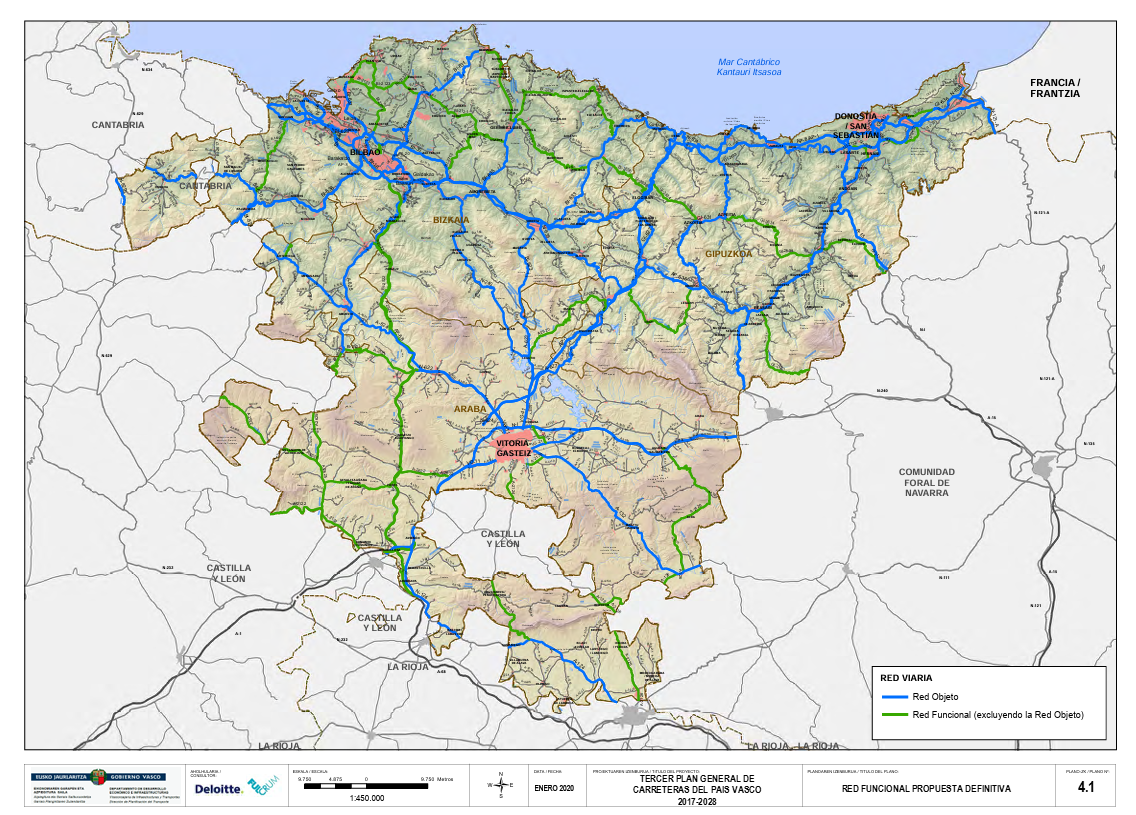
\includegraphics[scale=0.5]{includes/red_viaria_capv.png}
	\caption[Red viaria de la CAPV, extraído del Tercer Plan General de Carreteras del País Vasco 2017-2028. Fuente: https://www.euskadi.eus/tercer-plan-general-de-carreteras-del-pais-vasco-2017-2028/web01-a2bideko/es/]{Red viaria de la CAPV}
	\label{fig:red_viaria}
\end{figure}


En la figura \ref{fig:red_viaria} se aprecia la complejidad de la red viaria en la \acrshort{capv}. En diversas zonas como los accesos a Bilbao, los túneles del Kadagua o los enlaces con la A-8, se producen episodios de congestión recurrentes, especialmente en horas punta y durante condiciones meteorológicas adversas. Aunque Bizkaia dispone de una infraestructura \acrshort{its} notable (sensores, cámaras, estaciones meteorológicas), no se cuenta aún con herramientas predictivas suficientemente precisas que permitan anticipar estos episodios y facilitar la toma de decisiones en tiempo real.

La complejidad inherente a los datos de tráfico, caracterizados por correlaciones espacio-temporales, no linealidades y gran volumen, exige modelos capaces de capturar dichas relaciones con eficacia. Las aproximaciones tradicionales, basadas en regresión o aprendizaje automático clásico, resultan insuficientes en este contexto. Se necesita un enfoque moderno, capaz de integrar múltiples fuentes de datos y aprender representaciones complejas.

En respuesta a los retos mencionados, este trabajo propone el diseño, desarrollo y evaluación de un modelo de predicción del tráfico en Bizkaia basado en redes neuronales con arquitectura Transformer. Esta arquitectura ha demostrado un rendimiento sobresaliente en tareas de modelado secuencial y captura de dependencias a largo plazo, gracias a su mecanismo de atención, lo que la convierte en una candidata idónea para abordar la predicción de tráfico con alta precisión.

El modelo se alimentará de datos abiertos sobre tráfico y meteorología, publicados por organismos como Open Data Euskadi y Euskalmet, lo que garantiza la transparencia, replicabilidad y aplicabilidad del sistema propuesto. A través de un enfoque empírico, se evaluará la eficacia del modelo frente a enfoques tradicionales, utilizando métricas estándar y se estudiará su potencial para integrarse en sistemas actuales de gestión del tráfico.

Este documento se estructura de la siguiente manera: el capítulo 2 presenta una revisión del estado del arte, analizando los principales trabajos relacionados y su aplicabilidad al contexto de Bizkaia; el capítulo 3 define los objetivos del trabajo y la metodología seguida; los capítulos siguientes abordarán el desarrollo del proyecto y conclusiones finales, aunque esto es un trabajo por determinar.

\subsection{Introducción general del trabajo}

\vspace*{\fill}
\selectlanguage{spanish}
\begin{abstract}
	La predicción precisa del tráfico es clave para optimizar la movilidad y el uso de infraestructuras, especialmente en la \acrlong{capv} y más en concreto en la provincia de Bizkaia, donde la orografía, densidad urbana y condiciones meteorológicas suponen retos añadidos. Sin embargo, la complejidad inherente a los datos de tráfico, caracterizados por fuertes correlaciones espacio-temporales y patrones no lineales, dificulta su modelado y predicción exacta. Este trabajo propone un modelo de predicción basado en redes neuronales con arquitectura Transformer, capaz de capturar dependencias espacio-temporales complejas mediante mecanismos de atención que asignan pesos dinámicos a segmentos relevantes. Se emplearán datos abiertos de tráfico y meteorología procedentes de la provincia de Bizkaia. La validación se realizará con datos reales y se comparará frente a modelos tradicionales de redes neuronales, demostrando mejoras significativas en precisión. El sistema resultante ofrece una herramienta robusta y eficiente para la gestión del tráfico en tiempo real, con potencial para anticipar congestiones y optimizar la toma de decisiones operativas.
\end{abstract}
\textbf{Palabras clave}: Predicción del tráfico, Aprendizaje profundo, Transformers, Redes neuronales, Correlación espacio-temporal, Datos abiertos, Comunidad Autónoma del País Vasco, Bizkaia

\vfill

\selectlanguage{english}

\begin{abstract}
	Accurate traffic forecasting is essential for optimising mobility and infrastructure usage, especially in the Autonomous Community of the Basque Country (\acrshort{capv}) and particularly in the province of Bizkaia, where the region’s orography, urban density, and weather variability present additional challenges. However, the inherent complexity of traffic data, characterised by strong spatio-temporal correlations and non-linear patterns, makes its modelling and prediction difficult. This work proposes a prediction model based on neural networks with Transformer architecture, capable of capturing complex spatio-temporal dependencies through attention mechanisms that dynamically assign weights to relevant segments. Bizkaia's open traffic and weather datasets will be used. The model will be validated with real-world data and compared against traditional neural network models. The outcome will be a robust and efficient tool for real-time traffic management, with the potential to anticipate congestion and support the optimisation of operational decision-making.
\end{abstract}

\textbf{Keywords}: Traffic forecasting, Deep learning, Transformers, Neural networks, Spatio-temporal correlation, Open data, Autonomous Community of the Basque Country, Bizkaia
\selectlanguage{spanish}
\vspace*{\fill}
	\clearpage
	\section*{Contexto y estado del arte}
\label{sec:ctx_estart}
\addcontentsline{toc}{section}{Contexto y estado del arte}

En los últimos años, la predicción del tráfico se ha convertido en un campo de investigación clave dentro de los \acrlong{its}, impulsado por la disponibilidad creciente de datos en tiempo real y los avances en el aprendizaje automático. El objetivo principal es anticipar las condiciones del tráfico con suficiente precisión como para facilitar la toma de decisiones, tanto por parte de los operadores como de los usuarios de la red vial.

La problemática de la predicción del tráfico en entornos urbanos y regionales como Bizkaia presenta una elevada complejidad, debido a la naturaleza altamente dinámica y no lineal del flujo vehicular, así como por la influencia de factores exógenos como el clima, los eventos especiales o los accidentes. Esta complejidad ha motivado el desarrollo de una gran variedad de enfoques, desde modelos estadísticos clásicos hasta sofisticadas arquitecturas de aprendizaje profundo.

Este capítulo tiene como objetivo ofrecer un panorama de las principales técnicas, modelos y tecnologías utilizadas en la predicción del tráfico. A partir de una revisión sistemática de la literatura científica más relevante, se presentarán los enfoques predominantes y se analizará su aplicabilidad al caso concreto de Bizkaia. Finalmente, se establecerá un marco comparativo que servirá como punto de partida para justificar la solución propuesta en este trabajo.

\subsection{Técnicas existentes para la predicción del tráfico}

La literatura especializada distingue entre dos grandes familias de métodos para la predicción del tráfico: los modelos basados en estadística y los modelos basados en aprendizaje automático, con especial atención a los métodos de aprendizaje profundo. A continuación, se presenta una clasificación preliminar de las principales técnicas utilizadas:

\begin{itemize}
	\item \textbf{Modelos estadísticos}: \acrlong{arima}, Kalman Filter, regresiones lineales.
	\item \textbf{Modelos clásicos de machine learning}: \acrlong{svr}, \acrlong{rf}, \acrlong{knn}.
	\item \textbf{Redes neuronales profundas}:
	\begin{itemize}
		\item \acrlong{rnn}, \acrlong{lstm} y \acrlong{gru}.
		\item \acrlong{cnn}, para capturar relaciones espaciales.
		\item \acrlong{gnn}, incluyendo \acrlong{gcn} y \acrlong{gat}, adaptadas a redes viarias.
		\item Modelos Transformer.
	\end{itemize}
\end{itemize}

En las siguientes secciones, se revisarán con más detalle los fundamentos y aplicaciones de estas técnicas, poniendo el foco en los trabajos más relevantes que hayan utilizado estos enfoques en entornos comparables al del presente proyecto.

\subsubsection{Modelos estadísticos tradicionales}

Los modelos estadísticos tradicionales han sido fundamentales en la predicción del tráfico, especialmente en contextos donde se dispone de datos históricos limitados o se requiere una interpretación sencilla de los resultados. Estos modelos, incluyendo ARIMA, filtros de Kalman y regresiones lineales, permiten capturar patrones temporales y tendencias en los datos de tráfico, ofreciendo una base sólida para el desarrollo de sistemas de transporte inteligentes.

Los modelos \acrlong{arima} son herramientas estadísticas utilizadas para analizar y predecir series temporales. En el ámbito del tráfico, han demostrado ser eficaces para prever flujos vehiculares a corto plazo, especialmente en situaciones con patrones estacionales o tendencias lineales.

Por ejemplo, \cite{forecastArimaLtsm} aplicaron modelos \acrshort{arima} y \acrshort{lstm} para predecir el flujo de tráfico en la intersección de Muhima, Kigali, concluyendo que la combinación de ambos modelos mejora la precisión de las predicciones.

Asimismo, \cite{forecastSarima} propusieron un esquema de predicción utilizando el modelo \acrlong{sarima} para prever el flujo de tráfico a corto plazo con datos limitados, demostrando que es posible obtener predicciones precisas utilizando solo tres días de datos históricos.

El filtro de Kalman es un algoritmo recursivo que estima el estado de un sistema dinámico a partir de una serie de mediciones observadas, que contienen ruido y otras inexactitudes. En la predicción del tráfico, se utiliza para estimar y prever el flujo vehicular en tiempo real, adaptándose a cambios abruptos y condiciones variables.​

\cite{forecastKalman} emplearon el filtro de Kalman para predecir el flujo de tráfico a corto plazo en una carretera urbana de Dhaka, Bangladesh. El modelo logró un \acrlong{mape} del 14.62\%, indicando una precisión aceptable para aplicaciones prácticas.

La regresión lineal es una técnica estadística que modela la relación entre una variable dependiente y una o más variables independientes. En el contexto del tráfico, se ha utilizado para prever velocidades y flujos vehiculares basándose en variables como el tiempo, la densidad y la ocupación de la vía.​

Por ejemplo, \cite{liu2020congestion} desarrollaron un modelo de predicción del tiempo de congestión del tráfico utilizando análisis de regresión múltiple y análisis de supervivencia. El estudio demostró que el modelo de regresión lineal múltiple puede predecir con precisión el tiempo de congestión del tráfico, con un grado de ajuste entre el valor predicho y el valor real superior a 0.96. Este enfoque permitió identificar las características de distribución y duración de la congestión, proporcionando una base sólida para la predicción del tráfico en entornos urbanos.​

Sin embargo, estudios recientes han señalado limitaciones en la regresión lineal para capturar relaciones no lineales complejas en los datos de tráfico. Por ejemplo, en un análisis exhaustivo, se comparó el rendimiento de la regresión lineal con modelos más avanzados como \acrlong{rf} y XGBoost, encontrando que la regresión lineal presenta un ajuste deficiente y errores significativos en la predicción de velocidades de tráfico.

\subsubsection{Modelos clásicos de Machine Learning}

Los modelos clásicos de machine learning son métodos estadísticos avanzados capaces de abordar problemas complejos y no lineales. A continuación se describen brevemente tres técnicas destacadas: \acrlong{svr}, \acrlong{rf} y \acrlong{knn}, incluyendo ejemplos recientes de aplicaciones en la predicción del tráfico.

En cuanto a \acrfull{svr}, es una técnica basada en \acrfull{svm} que utiliza una función kernel para transformar el espacio de entrada original a uno de mayor dimensión, permitiendo modelar relaciones no lineales. El objetivo del \acrshort{svr} es identificar una función que tenga, como máximo, un error preestablecido (denominado \textit{margen}) respecto a los datos reales.

En el contexto de predicción de tráfico, \acrshort{svr} se ha mostrado eficaz debido a su robustez ante ruido y capacidad de generalización con muestras pequeñas. Por ejemplo, un estudio reciente aplicó \acrshort{svr} para predecir el volumen de tráfico a corto plazo utilizando datos de flujo vehicular recolectados en áreas urbanas, mostrando una precisión significativa en comparación con métodos \acrshort{lstm} de \cite{omar2024}.

\acrfull{rf} es un algoritmo basado en árboles de decisión, que genera múltiples árboles de forma independiente, utilizando subconjuntos aleatorios de datos de entrenamiento (bagging) y variables aleatorias. La predicción final se obtiene por consenso, promediando las predicciones individuales de cada árbol, lo que reduce considerablemente el riesgo de sobreajuste.

En el ámbito del tráfico, \acrshort{rf} es capaz de manejar grandes volúmenes de datos y capturar relaciones no lineales y complejas. Un ejemplo de aplicación es el estudio realizado por \cite{forecastRf}. El estudio tiene como objetivo predecir el flujo de tráfico a corto plazo, considerando patrones espaciales y temporales. Tras el preprocesamiento de datos con el Transformador Cuantil y la exploración de la correlación del flujo de tráfico, se identificaron los hiperparámetros óptimos del modelo mediante la búsqueda de cuadrícula de validación cruzada. El modelo \acrshort{rf} demostró el mejor rendimiento, alcanzando una alta precisión en la predicción del flujo de tráfico.

\acrfull{knn} es uno de los algoritmos más sencillos dentro de los métodos de aprendizaje supervisado. Este método predice el valor de una observación nueva en función de los valores de las K observaciones más cercanas del conjunto de entrenamiento. La cercanía se determina generalmente mediante una métrica de distancia, siendo la distancia euclidiana la más comúnmente utilizada.

A pesar de su simplicidad, \acrshort{knn} es muy eficaz en la predicción de tráfico cuando los patrones de flujo muestran alta dependencia espacial y temporal. Recientemente, \cite{forecastKnn} emplearon \acrshort{knn} para la predicción del tráfico en Bandung, Indonesia, empleando este método e integrado con la aplicación de simulación de movilidad urbana SUMO. El estudio buscó mitigar la congestión de tráfico anual en la ciudad, particularmente en periodos vacacionales. Utilizaron datos históricos de tráfico de Jl. Riau Bandung para predecir el nivel de congestión. La evaluación del rendimiento del método, usando una división de datos para entrenamiento y prueba, demostró una precisión muy alta con diferentes valores de 'k' vecinos considerados.

\subsubsection{Aprendizaje profundo}

El \textit{Deep Learning} o aprendizaje profundo es un área de \textit{Machine Learning} que utiliza redes neuronales artificiales de múltiples capas para modelar patrones complejos en los datos. Tras varias décadas de relativo estancamiento debido a las limitaciones computacionales y a las críticas vertidas por Minsky y Papert en los años 60 en el libro \textit{Perceptrons: An Introduction to Computational Geometry} \cite{minsky1969perceptrons}, las redes neuronales experimentaron un resurgimiento a partir de la década de los 2000, impulsado por el incremento exponencial de la capacidad de cómputo, la disponibilidad de grandes volúmenes de datos y el avance en algoritmos de entrenamiento. Este renacimiento del interés en las redes profundas se consolidó con el trabajo de \cite{hinton2006reducing}, donde se introdujo una técnica de preentrenamiento capa por capa utilizando autoencoders y máquinas de Boltzmann restringidas para facilitar el entrenamiento de redes neuronales profundas.

Sin embargo, fue en 2012 cuando el aprendizaje profundo irrumpió definitivamente en la comunidad científica, con la publicación de AlexNet, una red convolucional profunda que ganó con gran margen la competición ImageNet Large Scale Visual Recognition Challenge (ILSVRC). En este trabajo, Krizhevsky, Sutskever y Hinton demostraron que las redes profundas entrenadas con \acrlong{gpu} podían superar ampliamente los métodos tradicionales en tareas de visión por computador \cite{krizhevsky2012imagenet}. Este hito marcó el inicio de una nueva era para el aprendizaje profundo, consolidándolo como una de las herramientas más poderosas dentro del campo de la inteligencia artificial.

Actualmente, el aprendizaje profundo se caracteriza por la capacidad de representar funciones no lineales muy complejas gracias a estructuras como las redes neuronales profundas de tipo \acrlong{mlp}. Estas redes constan de múltiples capas ocultas, donde cada capa procesa información progresivamente más abstracta y permite descubrir patrones intrínsecos en grandes volúmenes de datos.

\subsubsection{Redes neuronales recurrentes}

Dentro del aprendizaje profundo, una clase especial de redes neuronales, conocidas como \acrfull{rnn}, ha demostrado ser particularmente efectiva para modelar secuencias temporales. Las \acrshort{rnn} están diseñadas para capturar dependencias temporales a largo plazo gracias a su estructura recurrente, que permite que la salida de una etapa de la red influya en etapas posteriores.

Las variantes más importantes y populares de las \acrshort{rnn} son las redes \acrlong{lstm} y \acrlong{gru}. Las \acrshort{lstm} fueron propuestas por \cite{hochreiter1997long}, y están especialmente diseñadas para manejar el problema del desvanecimiento del gradiente mediante el uso de puertas que controlan la información almacenada en la memoria de la red. Por otro lado, las redes \acrshort{gru}, introducidas por \cite{cho2014gru}, simplifican el modelo \acrshort{lstm} al combinar algunas de sus puertas, proporcionando un rendimiento similar con menos parámetros y una complejidad computacional reducida.

Diversos estudios han aplicado exitosamente las redes neuronales recurrentes a problemas específicos de predicción de tráfico, destacando las arquitecturas \acrshort{lstm} y \acrshort{gru}.

Un ejemplo notable es el trabajo realizado por \cite{zhao2017lstm}, en el que utilizaron una red neuronal \acrshort{lstm} para la predicción de flujo de tráfico a corto plazo. En su investigación, entrenaron un modelo con datos históricos de volumen vehicular recolectados en sensores, alcanzando un \acrfull{mre} de tan solo un 6,41\%, demostrando así la efectividad del enfoque \acrshort{lstm} para capturar patrones complejos en series temporales del tráfico.

En cuanto a la aplicación de redes \acrshort{gru}, cabe destacar el estudio llevado a cabo por \cite{ma2022cnn_gru}, quienes diseñaron un algoritmo híbrido basado en la combinación de \acrshort{cnn} y \acrshort{gru} para predecir la velocidad del tráfico. Este modelo obtuvo una media del \acrshort{mape} de aproximadamente 8,60\%, reflejando una considerable precisión en la predicción del flujo vehicular al integrar tanto características espaciales como temporales del tráfico.

Ambos estudios evidencian cómo el uso de redes neuronales recurrentes permite modelar con alta precisión las dependencias temporales complejas inherentes al tráfico vehicular, posicionándolas como una alternativa destacada frente a métodos clásicos o más tradicionales. Estos modelos son especialmente útiles en contextos de predicción a corto plazo, donde la precisión y la velocidad de respuesta son críticas para una gestión eficiente del tráfico y la toma de decisiones en tiempo real.

\begin{comment}
\subsubsection{Redes convolucionales}

Las \acrlong{cnn} son una clase de modelos de aprendizaje profundo diseñados para procesar datos con una estructura de tipo rejilla, como imágenes o series temporales espaciales. Su arquitectura se compone de capas convolucionales que aplican filtros para extraer características locales, seguidas de capas de agrupamiento y, finalmente, capas completamente conectadas para la toma de decisiones.​

En el contexto del tráfico vehicular, las \acrshort{cnn} son particularmente útiles para modelar la relación espacial entre diferentes segmentos de carretera y capturar patrones temporales en los datos de flujo de tráfico. Al representar los datos de tráfico en forma de matrices que reflejan la intensidad del tráfico en diferentes ubicaciones y momentos, las \acrshort{cnn} pueden aprender representaciones jerárquicas que facilitan la predicción precisa del flujo de tráfico.

La predicción precisa del flujo de tráfico es esencial para la gestión eficiente de las redes de transporte. Las \acrshort{cnn} permiten modelar las complejas interacciones espaciales y temporales presentes en los datos de tráfico, lo que resulta en predicciones más precisas y robustas. Además, su capacidad para manejar grandes volúmenes de datos y aprender características discriminativas las hace adecuadas para aplicaciones en tiempo real y sistemas de transporte inteligentes.

En el estudio \textit{WT-2DCNN: A convolutional neural network traffic flow prediction model} los autores \cite{forecastCnnWavelet} proponen un modelo que combina la transformada wavelet para la reconstrucción y descomposición de datos con una red neuronal convolucional bidimensional (2DCNN). Este enfoque permite manejar el ruido presente en los datos de tráfico y capturar características espaciales y temporales de manera más efectiva.​

La metodología aplicada consistía en los siguientes pasos. Para empezar, se aplica la transformada de wavelet para descomponer los datos de tráfico en componentes de diferentes frecuencias. Posteriormente, usa una 2DCNN para aprender las representaciones espaciales y temporales de los datos descompuestos y, para finalizar, se fusionan las características aprendidas para realizar la predicción del flujo del tráfico.

En consecuencia, el modelo WT-2DCNN demostró una mejora significativa en la precisión de la predicción del flujo de tráfico en comparación con métodos tradicionales, especialmente en escenarios con datos ruidosos.

En otro artículo científico titulado \textit{MF-CNN: Traffic Flow Prediction Using Convolutional Neural Network and Multi-Features Fusion}, los autores \cite{forecastMfCnn} presentan un modelo que integra múltiples características espaciales y temporales, así como factores externos como el clima y los días festivos, utilizando una red CNN para la predicción del flujo de tráfico.​

La metodología aplicada comienza por la extracción de características temporales a corto y largo plazo del flujo de tráfico. Seguidamente, se representan las características en matrices bidimensionales combinando dimensiones espaciales y temporales. A continuación, se aplica una \acrshort{cnn} para aprender las representaciones de las matrices y se finaliza fusionando las características aprendidas con factores externos mediante una capa de regresión logística para efectuar la predicción final.

Como resultado, el modelo MF-CNN logró una mejora notable en la precisión de la predicción del flujo de tráfico en comparación con varios modelos de referencia, demostrando la efectividad de integrar múltiples características y factores externos en el proceso de predicción.​
\end{comment}

\subsubsection{Graph Neural Networks}

Las \acrlong{gnn} surgen de la necesidad de extender las capacidades del aprendizaje profundo a datos no euclidianos, como los grafos, que representan relaciones complejas entre entidades. A diferencia de las redes neuronales tradicionales, que operan sobre datos estructurados en rejillas (como imágenes o secuencias), las \acrshort{gnn} están diseñadas para trabajar directamente con la estructura de los grafos, tal y como se explica por \cite{theoryGnn}, permitiendo capturar dependencias tanto locales como globales entre nodos.

Las GNN se basan en el principio de \textit{message passing}, donde cada nodo actualiza su representación en función de sus vecinos. Entre las arquitecturas más destacadas se encuentran:​

\begin{itemize}
	\item \textbf{\acrlong{gcn}}: Fueron introducidas en \cite{theoryGcn}. Estas redes generalizan las convoluciones a grafos, permitiendo una agregación eficiente de la información de los vecinos.
	\item \textbf{\acrlong{gat}}: Incorporan mecanismos de atención (como se verá más adelante) para ponderar la importancia de cada vecino en la actualización del nodo central. Fueron introducidas en \cite{theoryGan}.
	\item \textbf{\acrlong{ggnn}}: Utilizan mecanismos de puertas, similares a las \acrshort{lstm}, para controlar el flujo de información entre nodos.
\end{itemize}

La predicción del flujo de tráfico es un desafío clave en los sistemas de transporte inteligentes, donde es esencial anticipar las condiciones del tráfico para optimizar la movilidad urbana. Las \acrshort{gnn} son particularmente adecuadas para esta tarea debido a que las redes de carreteras pueden modelarse naturalmente como grafos, donde los nodos representan intersecciones o sensores, y las aristas representan las conexiones viales.

Un estudio destacado en este ámbito es \textit{Improving Traffic Density Forecasting in Intelligent Transportation Systems Using Gated Graph Neural Networks}, de \cite{forecastGgnn}. En este trabajo, los autores comparan diferentes arquitecturas de \cite{gnn} para la predicción de la densidad del tráfico, incluyendo \acrshort{gcn}, GraphSAGE y \acrshort{ggnn}. Los resultados muestran que las acrshort superan a las demás arquitecturas en términos de precisión, con un RMSE de 9.15 y un MAE de 7.1, destacando su capacidad para capturar dinámicamente las dependencias espaciales y temporales en los datos de tráfico.​

Otro estudio relevante es \textit{TrafficStream: A Streaming Traffic Flow Forecasting Framework Based on Graph Neural Networks and Continual Learning} de \cite{forecastGnn}. Este trabajo propone un marco de predicción de flujo de tráfico en tiempo real que combina \acrshort{gnn} con aprendizaje continuo, permitiendo adaptarse a cambios en la red de tráfico y patrones de flujo a lo largo del tiempo. El modelo utiliza estrategias como la reactivación de datos históricos y el suavizado de parámetros para mantener la precisión de las predicciones en entornos dinámicos.​

\subsubsection{Redes Neuronales con Transformers}

El avance hacia modelos más potentes y versátiles dentro del aprendizaje profundo encontró un punto de inflexión crucial en 2017 con la publicación del influyente artículo \textit{Attention is all you need} por \cite{attentionIsAllYouNeed}. Esta publicación revolucionó el campo del aprendizaje automático al introducir la arquitectura Transformer, una propuesta que eliminaba por completo el uso de estructuras recurrentes como \acrshort{rnn} o \acrshort{lstm}, en favor de un novedoso mecanismo de atención que permitía modelar relaciones de largo alcance en las secuencias de entrada, mediante el cómputo paralelo.

La clave de los Transformers reside en el \textbf{multi-head self-attention}, que otorga al modelo la capacidad de ponderar dinámicamente la importancia relativa de distintos elementos dentro de una secuencia. Este mecanismo, además de ofrecer un rendimiento computacional más eficiente, mejora la capacidad de aprendizaje del modelo frente a secuencias largas o ruidosas, lo que resulta particularmente útil en dominios complejos como la predicción del flujo del tráfico urbano.

A diferencia de las \acrshort{rnn}, que deben procesar las secuencias de manera secuencial, los Transformers permiten el aprendizaje paralelo y la captura simultánea de dependencias tanto locales como globales, lo que ha demostrado ser especialmente relevante para modelar patrones espacio-temporales complejos.

\vspace{0.5cm}

El uso de modelos Transformer en el ámbito de los sistemas inteligentes de transporte ha crecido significativamente en los últimos años, debido a su capacidad para capturar interacciones complejas entre nodos de una red vial y su evolución en el tiempo.

Un estudio reciente y particularmente relevante para este trabajo es el desarrollado por \cite{trafficformer}, titulado \textit{Transformer-based short-term traffic forecasting model considering traffic spatiotemporal correlation}. En este artículo, los autores presentan \textbf{Trafficformer}, un modelo Transformer adaptado específicamente a la predicción del tráfico a corto plazo, integrando correlaciones espacio-temporales mediante máscaras espaciales y representaciones topológicas de la red viaria.

En cuanto a la arquitectura, el modelo Trafficformer consta de tres módulos fundamentales: 
\begin{itemize}
	\item[(1)] Extracción de características temporales mediante \acrlong{mlp}. 
	\item[(2)] Interacción espacial basada en codificadores Transformer con máscaras de atención topológicas. 
	\item[(3)] Predicción de velocidades mediante una red \acrshort{mlp} final. 
\end{itemize}

Esta arquitectura fue evaluada con el conjunto de datos del \textit{Seattle Loop Detector Dataset}, superando a modelos clásicos como ARIMA, \acrshort{svr} y también a redes profundas como \acrshort{lstm}+\acrshort{mlp} y TGG-LSTM, tanto en precisión (\acrshort{mae}, \acrshort{mape}, \acrshort{rmse}) como en eficiencia computacional.

La inclusión de una máscara espacial, que filtra interacciones irrelevantes basándose en la topología vial y el tiempo de viaje entre nodos, permitió al modelo enfocarse en relaciones espacialmente significativas, lo que se tradujo en una mejora del 18\% en precisión frente a modelos equivalentes sin esta optimización. Esta capacidad de interpretar relaciones espaciales relevantes es fundamental en contextos como el tráfico urbano, donde las dependencias no son uniformes ni euclidianas, y dependen del trazado real de la red viaria.

\vspace{0.5cm}

El trabajo de \cite{trafficformer} demuestra que los modelos basados en Transformers no sólo son competitivos, sino que se posicionan como una opción de referencia para tareas de predicción del tráfico, permitiendo una mejor generalización, mayor interpretabilidad y adaptabilidad frente a cambios dinámicos en la red.

Este enfoque supone un salto cualitativo respecto a técnicas previas como \acrshort{lstm}, \acrshort{gru} o incluso \acrshort{gnn}, al combinar lo mejor de los modelos de secuencia (captura temporal) con mecanismos estructurados de atención espacial. Además, su arquitectura modular y altamente paralelizable lo convierte en un candidato ideal para despliegues en entornos cloud, edge o híbridos, como los requeridos en la infraestructura del proyecto que nos ocupa.

Por todo ello, este modelo ha sido seleccionado como piedra angular sobre la cual se desarrollará la propuesta metodológica del presente trabajo, tanto en la fase de experimentación como en el diseño arquitectónico del modelo final.

\subsection{Ventajas del uso de Transformers frente a otras arquitecturas}

La arquitectura Transformer representa un avance significativo respecto a los modelos secuenciales (\acrshort{lstm} o \acrshort{gru}) y estructurales (como las \acrshort{gnn}), tanto desde el punto de vista teórico como práctico.

En primer lugar, los modelos secuenciales dependen fuertemente del procesamiento secuencial, lo que limita la paralelización durante el entrenamiento y puede llevar a problemas de desvanecimiento o explosión del gradiente (leer en \cite{desvGradiente}) en secuencias largas. Aunque han demostrado buen rendimiento en predicción temporal, su capacidad para modelar relaciones espaciales complejas es limitada. Por otro lado, las \acrshort{gnn} destacan en la modelización espacial, pero presentan dificultades cuando se requiere combinar relaciones topológicas con dinámicas temporales de forma eficaz.

Los Transformers, y en particular la arquitectura Trafficformer, superan estas limitaciones al:

\begin{itemize}
	\item \textbf{Separar explícitamente los componentes espaciales y temporales}: Trafficformer utiliza una \acrshort{mlp} para extracción temporal y un codificador Transformer para interacción espacial, optimizando cada fase por separado.
	\item \textbf{Utilizar multi-head self-attention con enmascaramiento espacial}: Esto permite al modelo centrarse solo en las interacciones viales relevantes, mejorando la eficiencia y la precisión.
	\item \textbf{Permitir entrenamiento completamente paralelo}: Gracias al mecanismo de atención, el modelo puede ser entrenado de manera más rápida que una \acrshort{rnn} convencional.
\end{itemize}

Los resultados experimentales de \cite{trafficformer} muestran que Trafficformer supera consistentemente a las otras propuestas mencionadas anteriormente en múltiples métricas de evaluación como \acrshort{mae}, \acrshort{rmse} y \acrshort{mape}. Por ejemplo, en el dataset del \textit{Seattle Loop Detector}, se observó una mejora de hasta el 18\% en error medio absoluto frente a los mejores modelos recurrentes. Además, la arquitectura Transformer mostró una mayor capacidad de generalización frente a cambios dinámicos del tráfico. En la tabla \ref{tab:comparativa_modelos} se puede ver a modo resumido todo lo dicho anteriormente.

\begin{table}[H]
	\centering
	\caption{Comparativa entre arquitecturas en tareas de predicción del tráfico}
	\label{tab:comparativa_modelos}
	\renewcommand{\arraystretch}{1.4}
	\begin{tabularx}{\textwidth}{lXXX}
		\toprule
		\textbf{Aspecto} & \textbf{RNNs (LSTM, GRU)} & \textbf{GNNs} & \textbf{Transformers} \\
		\midrule
		Procesamiento secuencial vs. paralelo &
		Procesamiento secuencial con paralelización limitada &
		No aplicable (estructura estática) &
		Paralelización total mediante mecanismo de atención \\
		
		\midrule
		Modelado espacial y temporal &
		Modelado temporal fuerte, pero poco eficiente para relaciones espaciales &
		Excelente modelado espacial, dificultad para integrar dinámica temporal &
		Modelado explícito y desacoplado de componentes espaciales y temporales \\
		
		\midrule
		Rendimiento empírico &
		Rendimiento limitado en benchmarks de tráfico &
		Rendimiento moderado en tareas espaciales, sensible a ruido temporal &
		Mejores resultados en métricas MAE, RMSE y MAPE, mayor capacidad de generalización \\
		\bottomrule
	\end{tabularx}
\end{table}

En resumen, los modelos Transformer no solo ofrecen ventajas computacionales, sino que proporcionan una representación más rica y eficiente de las correlaciones espacio-temporales que caracterizan al problema de la predicción del tráfico urbano. 
	\clearpage
	\section*{Objetivos y metodología de trabajo}
\label{sec:obj_metd}
\addcontentsline{toc}{section}{Objetivos y metodología de trabajo}

En este capítulo se exponen los objetivos perseguidos con el desarrollo del presente Trabajo Fin de Máster, pasando por la infraestructura y tecnologías seleccionadas, y acabando con la metodología empleada para su ejecución. El trabajo se enmarca dentro del área del aprendizaje profundo, aplicados al problema de la predicción del flujo de tráfico urbano. El propósito es diseñar una solución capaz de anticipar el estado de la red viaria a corto plazo en la provincia de Bizkaia, utilizando datos abiertos y públicos de fuentes institucionales, lo cual permitirá evaluar tanto la capacidad de generalización de los modelos como su utilidad práctica en un contexto real. 

Como se analizó en el capítulo anterior, la predicción del tráfico urbano enfrenta importantes retos derivados de la alta variabilidad temporal y la compleja dependencia espacial de los datos. Entre los trabajos analizados, destaca el modelo Trafficformer de \cite{trafficformer}, que introduce un enfoque basado en Transformers mejorado mediante máscaras espaciales para filtrar ruido y enfocar la atención en interacciones relevantes entre nodos de la red. Aunque el modelo original fue diseñado para predecir velocidades de tráfico, su arquitectura resulta igualmente aplicable a la predicción de volúmenes de tráfico, esto es, la cantidad de vehículos que circulan por un punto dado en cada intervalo temporal, mediante una adaptación del preprocesamiento y del objetivo del modelo.

\subsection{Objetivos del proyecto}

El objetivo general de este Trabajo Fin de Máster es el diseño, implementación y evaluación de un sistema de predicción del tráfico urbano a corto plazo mediante el uso de técnicas de aprendizaje profundo, con especial énfasis en las redes neuronales de tipo Transformer. La solución desarrollada debe ser capaz de predecir con precisión el estado futuro del tráfico en diversos puntos de la red viaria de Bizkaia, aprovechando el valor añadido que ofrecen los datos abiertos procedentes de fuentes públicas, como los portales de Open Data del Gobierno Vasco. Para ello, se debe implementar y entrenar un modelo de predicción inspirado en el modelo Trafficformer, adaptado a volúmenes de tráfico. Este objetivo principal responde a la necesidad creciente de disponer de herramientas tecnológicas que permitan mejorar la gestión de la movilidad en entornos urbanos, facilitar la toma de decisiones estratégicas y operativas en tiempo real, y anticiparse a situaciones potenciales de congestión. La precisión de la predicción se configura como un factor clave en la eficacia de sistemas \acrshort{its} modernos, especialmente en contextos densamente poblados como el área metropolitana de Bilbao. 

Como primer objetivo específico se pretende analizar el conjunto de datos disponibles en el catálogo de datos abiertos del Gobierno Vasco ubicado en \cite{openDataGv}. Dentro del mismo, se pretende identificar y analizar el Api de tráfico de \cite{apiTraffic}, además de otros factores contextuales como la meteorología, que se ha demostrado influyente en la dinámica del tráfico y cuyo \acrshort{api} se ubica en \cite{apiMeteo}.

Asimismo, se plantea como segundo objetivo específico la validación empírica de los modelos mediante experimentación con datos reales, evaluando su rendimiento con métricas reconocidas en el ámbito de la predicción, tales como el error cuadrático medio o \acrshort{rmse}, el error absoluto medio o \acrshort{mae} o el error porcentual absoluto medio o \acrshort{mape}. La comparación entre distintos enfoques permitirá identificar las ventajas y limitaciones de cada uno, así como proponer mejoras que potencien su aplicabilidad.

Por último, se considera el tercer objetivo específico del trabajo ofrecer una reflexión crítica sobre el impacto potencial de este tipo de soluciones en el ámbito de la movilidad urbana y su eventual integración en sistemas de ayuda a la decisión de carácter público o privado. El valor añadido que se pretende aportar no reside únicamente en la capacidad predictiva del modelo, sino también en su posible contribución al desarrollo de una movilidad más eficiente, sostenible e inteligente.

\subsection{Infraestructura y tecnologías empleadas}

En este apartado se van a exponer todos los recursos seleccionados que van a servir de soporte para la consecución de los objetivos y el desarrollo del proyecto.

Para ello, se va a utilizar una infraestructura híbrida compuesta por recursos locales y servicios en la nube.
Como equipo de desarrollo se va a seleccionar el equipo personal, que se compone por un procesador Intel Core i7-10700K de 10ª generación desbloqueado, con 32 GB de memoria \acrshort{ram} DDR4, haciendo uso de 2 discos \acrshort{ssd} NVMe (512 GB + 1 TB) y un HDD de 2 TB como almacenamiento, equipado con una GPU Nvidia GTX 1070 con soporte CUDA y corriendo el Sistema Operativo Windows 11 Pro.

Este equipo permitirá realizar tareas de programación, experimentación y entrenamiento preliminar, si bien se anticipa que no será suficiente para entrenar modelos de gran tamaño o con grandes cantidades de datos.

Por ello, se deberá emplear una infraestructura remota para realizar los distintos entrenamientos. Dada la necesidad de cómputo intensivo, se contempla el uso de una instancia EC2 en Amazon Web Services (AWS), con una AMI optimizada para entrenamiento de modelos con PyTorch (por ejemplo, la AMI de Deep Learning de AWS con soporte GPU Tesla T4 o V100). Esta infraestructura permitirá acelerar significativamente el proceso de entrenamiento y validación.

Asimismo, se va a hacer uso de un servidor doméstico con \href{https://www.truenas.com/}{TrueNAS} Scale Electric Eel como sistema operativo, equipado con un procesador Intel Core i5-7400 de 7ª generación, con 16 GB de RAM DDR4 y dos discos duros de 4 TB configurados en RAID 1. Este servidor albergará una base de datos \href{https://www.mongodb.com/}{MongoDB} para almacenamiento estructurado de datos y \href{https://min.io/}{MinIO} como sistema de almacenamiento tipo S3, útil para almacenamiento masivo y backups. Todos esos servicios van a funcionar como contenedores \href{https://www.docker.com/}{Docker}.

En cuanto al software, se van a seleccionar los lenguajes de programación \href{https://kotlinlang.org/}{Kotlin} (con \href{https://gradle.org/}{Gradle} como herramienta de construcción) y \href{https://www.python.org/}{Python} (con \href{https://python-poetry.org/}{Poetry} como gestor de dependencias y de empaquetamiento). En cuanto a los entornos de desarrollo, se ha decidido hacer uso de la suite de Jetbrains, puesto que facilitan licencias para estudiantes y son muy completas (ofreciendo muchas funcionalidades y asistentes que hacen más productiva tu jornada). Estos IDE son \href{https://www.jetbrains.com/es-es/idea/}{IntelliJ IDEA} (para el desarrollo con Kotlin) y \href{https://www.jetbrains.com/es-es/pycharm/}{PyCharm} (para el desarrollo con Python). Para el control de versiones se va a emplear \href{https://git-scm.com/}{Git}, con repositorios en GitHub o GitLab.

Para el desarrollo del modelo de predicción de tráfico se ha optado por utilizar \href{https://pytorch.org/}{PyTorch} como backend principal. Esta decisión se fundamenta en la flexibilidad que ofrece esta biblioteca para la implementación de arquitecturas avanzadas, como redes neuronales recurrentes (LSTM, GRU), redes convolucionales (CNN), Graph Attention Networks (GAT) y modelos basados en Transformers. Además, PyTorch cuenta con una comunidad investigadora muy activa y un ecosistema maduro que incluye librerías especializadas como PyTorch Geometric o HuggingFace Transformers, altamente relevantes para el ámbito de este trabajo. A diferencia de otros entornos como TensorFlow/Keras, que destacan por su facilidad de uso en fases de prototipado, PyTorch ofrece un control más explícito sobre el flujo de datos y la personalización del entrenamiento, lo que resulta especialmente valioso en proyectos que requieren ajustar arquitecturas de manera específica para capturar correlaciones espaciotemporales complejas en el tráfico urbano. 

Estas decisiones se ven respaldadas por análisis comparativos recientes, como el realizado por DataCamp, donde se destaca que \textit{PyTorch} suele ser más rápido y proporciona mejores capacidades de depuración que \textit{Keras}. Estas características lo hacen especialmente adecuado para entornos de investigación y desarrollo de modelos complejos cite{datacamp2023}.

Además, UnfoldAI ofrece un análisis detallado sobre las fortalezas y debilidades de los principales frameworks de aprendizaje profundo. En su estudio comparativo se destaca que \textit{PyTorch} proporciona una mayor flexibilidad y control, lo que lo convierte en la opción preferida en entornos de investigación, mientras que \textit{Keras} sobresale por su simplicidad y facilidad de uso, resultando ideal para usuarios principiantes y tareas de prototipado rápido \cite{unfoldai2024}.

\subsection{Metodología de trabajo}

Para la consecución de los objetivos, tomando como referencia la solución Trafficformer, se ha pensado en estructurar el proyecto de la siguiente manera:

\begin{itemize}
	\item Adquisición y preprocesamiento de datos.
	\begin{itemize}
		\item \textbf{Datos}: se utilizarán datos abiertos provenientes del portal Open Data de Euskadi, principalmente de sensores que registran el número de vehículos que atraviesan puntos específicos de la red viaria en intervalos regulares.
		\item \textbf{Preprocesamiento}: se realizará la agregación temporal si es necesario (por ejemplo, a intervalos de 5 minutos), imputación de valores perdidos, normalización y generación de ventanas deslizantes para construir las series históricas.
	\end{itemize}
	\item Arquitectura del modelo. La arquitectura seguirá los principios del modelo Trafficformer, la cual se puede apreciar en la figura \ref{fig:trafficformer}, con los siguientes componentes adaptados:
	\begin{itemize}
		\item \textbf{Extracción temporal}: un MLP de dos capas se encargará de extraer patrones no lineales de las series de volumen de vehículos por punto de control.
		\item \textbf{Máscara espacial}: se construirá una matriz de adyacencia basada en la topología de la red viaria, utilizando distancias reales o tiempos de viaje para definir relaciones de vecindad relevantes.
		\item \textbf{Codificador Transformer}: mediante multi-head attention, el modelo extrae relaciones espaciales entre nodos cercanos, permitiendo una representación contextualizada del tráfico.
		\item \textbf{Predicción}: se proyectan las representaciones espacio-temporales a una predicción del número de vehículos que circularán por cada punto de la red en el siguiente intervalo.
	\end{itemize}
	\item Entrenamiento y evaluación.
	\begin{itemize}
		\item \textbf{Métricas}: se utilizarán MAE, RMSE y MAPE para comparar la predicción de conteos de vehículos.
		\item \textbf{Modelos base}: se tendrá como referencia el modelo \acrshort{mlp} desarrollado anteriormente.
		\item \textbf{Validación}: se aplicará validación temporal (walk-forward) para simular condiciones reales de predicción.
	\end{itemize}
\end{itemize}

\begin{figure}[H]
	\centering
	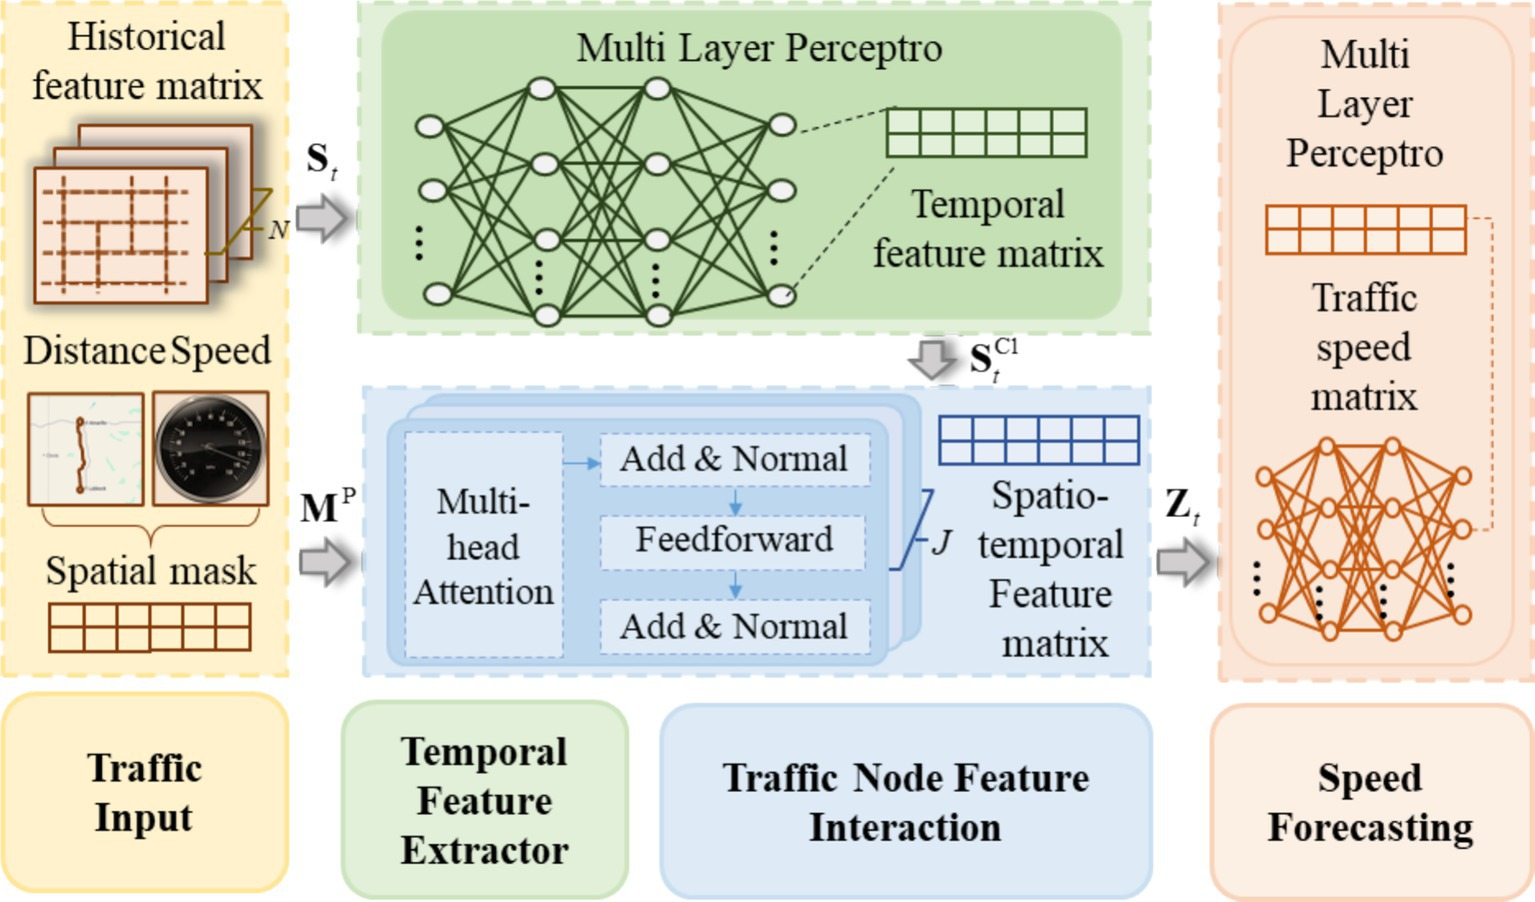
\includegraphics[width=0.9\textwidth]{includes/fnbot-19-1527908-g001.jpg}
	\caption{Arquitectura general del modelo Trafficformer \cite{trafficformer}}
	\label{fig:trafficformer}
\end{figure}

Como consecuencia, se prevé llevar a cabo las siguientes tareas.

\begin{itemize}
	\item Extracción y almacenamiento de datos. Desarrollo de un módulo en Kotlin para conectar con las \acrshort{api} públicas de tráfico y meteorología de Open Data Euskadi. Almacenamiento de los datos crudos en MongoDB y objetos binarios (imágenes, CSVs temporales) en MinIO.
	\item Preprocesamiento y transformación de datos. Conversión de datos crudos en estructuras listas para entrenamiento, mediante scripts en Python. Aplicación de técnicas de normalización, resampleo temporal y gestión de datos faltantes.
	\item Entrenamiento de modelos neuronales. Implementación de un modelo base \acrshort{mlp} para establecer una línea base de rendimiento. Posterior implementación de un modelo Transformer adaptado al tráfico, con atención espacio-temporal y uso de máscaras de conectividad vial.
	\item Evaluación comparativa. Evaluación de los modelos con un conjunto de métricas estándar (\acrshort{mae}, \acrshort{rmse}, \acrshort{mape}). Comparativa entre modelos para seleccionar el más adecuado para el caso de uso.
	\item Validación y conclusiones. Validación en escenarios reales y extracción de conclusiones sobre la utilidad del modelo. Estudio de la viabilidad de su aplicación en entornos reales, como el soporte a \acrshort{its} o planificación urbana.
\end{itemize}

	\clearpage
	\section{Construcción del dataset y arquitectura del sistema}
\label{sec:dataset_arquitectura}

%
% Para citar: 
% 	(ver Sección~\ref{sec:dataset_arquitectura})
% 	como se describe en la Sección~\nameref{sec:dataset_arquitectura})
%

En este capítulo se describe el diseño, desarrollo e implementación del sistema responsable de generar el dataset empleado en el modelo de predicción de tráfico. Se parte de la identificación y análisis de las fuentes de datos disponibles, que incluyen mediciones de flujo vehicular, condiciones meteorológicas e incidencias viales. A continuación, se detallan las decisiones técnicas adoptadas en la arquitectura del sistema de integración, los patrones de diseño utilizados y el procedimiento empleado para consolidar todas las observaciones en una única estructura homogénea: la clase \texttt{MobilitySnapshot}. Finalmente, se justifican aspectos clave como la granularidad temporal del dataset, los criterios de selección de variables y las estrategias de persistencia.


\subsection{Fuentes de datos y análisis de disponibilidad}

Durante la primera fase del proyecto, se realizó un análisis exhaustivo de las fuentes de datos abiertas disponibles para la provincia de Bizkaia en el ámbito de los \acrshort{its}. La fuente de datos principal se corresponde con el API de Tráfico del portal de Open Data del Gobierno Vasco \cite{apiTraffic}. Se identificaron tres orígenes principales de datos:

\begin{itemize}
	\item \textbf{Gobierno Vasco}: mediante el API de Open Data Euskadi, se obtuvo información de aforos de tráfico e incidencias viales.
	\item \textbf{Ayuntamiento de Bilbao}: también a través de Open Data, se extrajeron series temporales de datos de tráfico en tiempo real.
	\item \textbf{Diputación Foral de Bizkaia}: al no disponer de un endpoint público, se logró contactar con los técnicos responsables y obtener acceso a sus datos mediante ficheros descargables proporcionados manualmente.
\end{itemize}

La cobertura de los datos obtenidos se representa en la tabla \ref{tab:cobertura_datos_opendata}, extraída y adaptada de la documentación técnica del repositorio del proyecto.

\begin{table}[H]
	\centering
	\caption{Cobertura de datos por fuente y tipo.}
	\label{tab:cobertura_datos_opendata}
	\begin{comment}\renewcommand{\arraystretch}{1.2}\end{comment}
	\begin{tabularx}{\textwidth}{cXccc}
		\toprule
		\textbf{SourceId} & \textbf{Organización} & \textbf{Meters} & \textbf{Flows} & \textbf{Incidences} \\
		\midrule
		1 & Gobierno Vasco & \textcolor{mygreen}{\faCheck} & \textcolor{mygreen}{\faCheck} & \textcolor{mygreen}{\faCheck} \\
		2 & Diputación Foral de Bizkaia & \textcolor{gray}{\faHandPaper} & \textcolor{gray}{\faHandPaper} & \textcolor{mygreen}{\faCheck} \\
		3 & Diputación Foral de Álava & \textcolor{myred}{\faTimes} & \textcolor{myred}{\faTimes} & \textcolor{mygreen}{\faCheck} \\
		4 & Diputación Foral de Gipuzkoa & \textcolor{mygreen}{\faCheck} & \textcolor{myred}{\faTimes} & \textcolor{mygreen}{\faCheck} \\
		5 & Ayuntamiento Bilbao & \textcolor{mygreen}{\faCheck} & \textcolor{mygreen}{\faCheck} & \textcolor{mygreen}{\faCheck} \\
		6 & Ayuntamiento Vitoria-Gasteiz & \textcolor{mygreen}{\faCheck} & \textcolor{mygreen}{\faCheck} & \textcolor{mygreen}{\faCheck} \\
		7 & Ayuntamiento de Donostia-San Sebastián & \textcolor{mygreen}{\faCheck} & \textcolor{myred}{\faTimes} & \textcolor{mygreen}{\faCheck} \\
		\bottomrule
	\end{tabularx}
\end{table}

\begin{itemize}
	\item \textcolor{mygreen}{\faCheck} Datos existentes y descargados correctamente.
	\item \textcolor{myred}{\faTimes} No existen datos para ese \texttt{sourceId} en OpenData.
	\item \textcolor{gray}{\faHandPaper} Datos obtenidos de forma externa e introducidos manualmente mediante programación.
\end{itemize}

El presente caso de uso se circunscribe a la provincia de Bizkaia, por lo que únicamente se emplean las fuentes de datos identificadas con los códigos sourceId 1, 2 y 5. La fuente proporcionada por la Dirección de Tráfico del Gobierno Vasco abarca principalmente la red viaria principal de la Comunidad Autónoma del País Vasco (CAPV), incluyendo carreteras de alta capacidad. Por su parte, la base de datos de la Diputación Foral de Bizkaia recoge aforos situados, en su mayoría, en carreteras secundarias y forales. Finalmente, la fuente de datos del Ayuntamiento de Bilbao representa el entorno urbano, al contar con sensores ubicados en intersecciones y vías principales de la ciudad.

La Figura~\ref{fig:sourceid1_map} muestra la ubicación de los sensores de la fuente \texttt{source\_id = 1} (Gobierno Vasco). En muchos de estos puntos existen múltiples medidores, ya que se instala un sensor por carril en el mismo emplazamiento físico.

\begin{figure}[H]
	\centering
	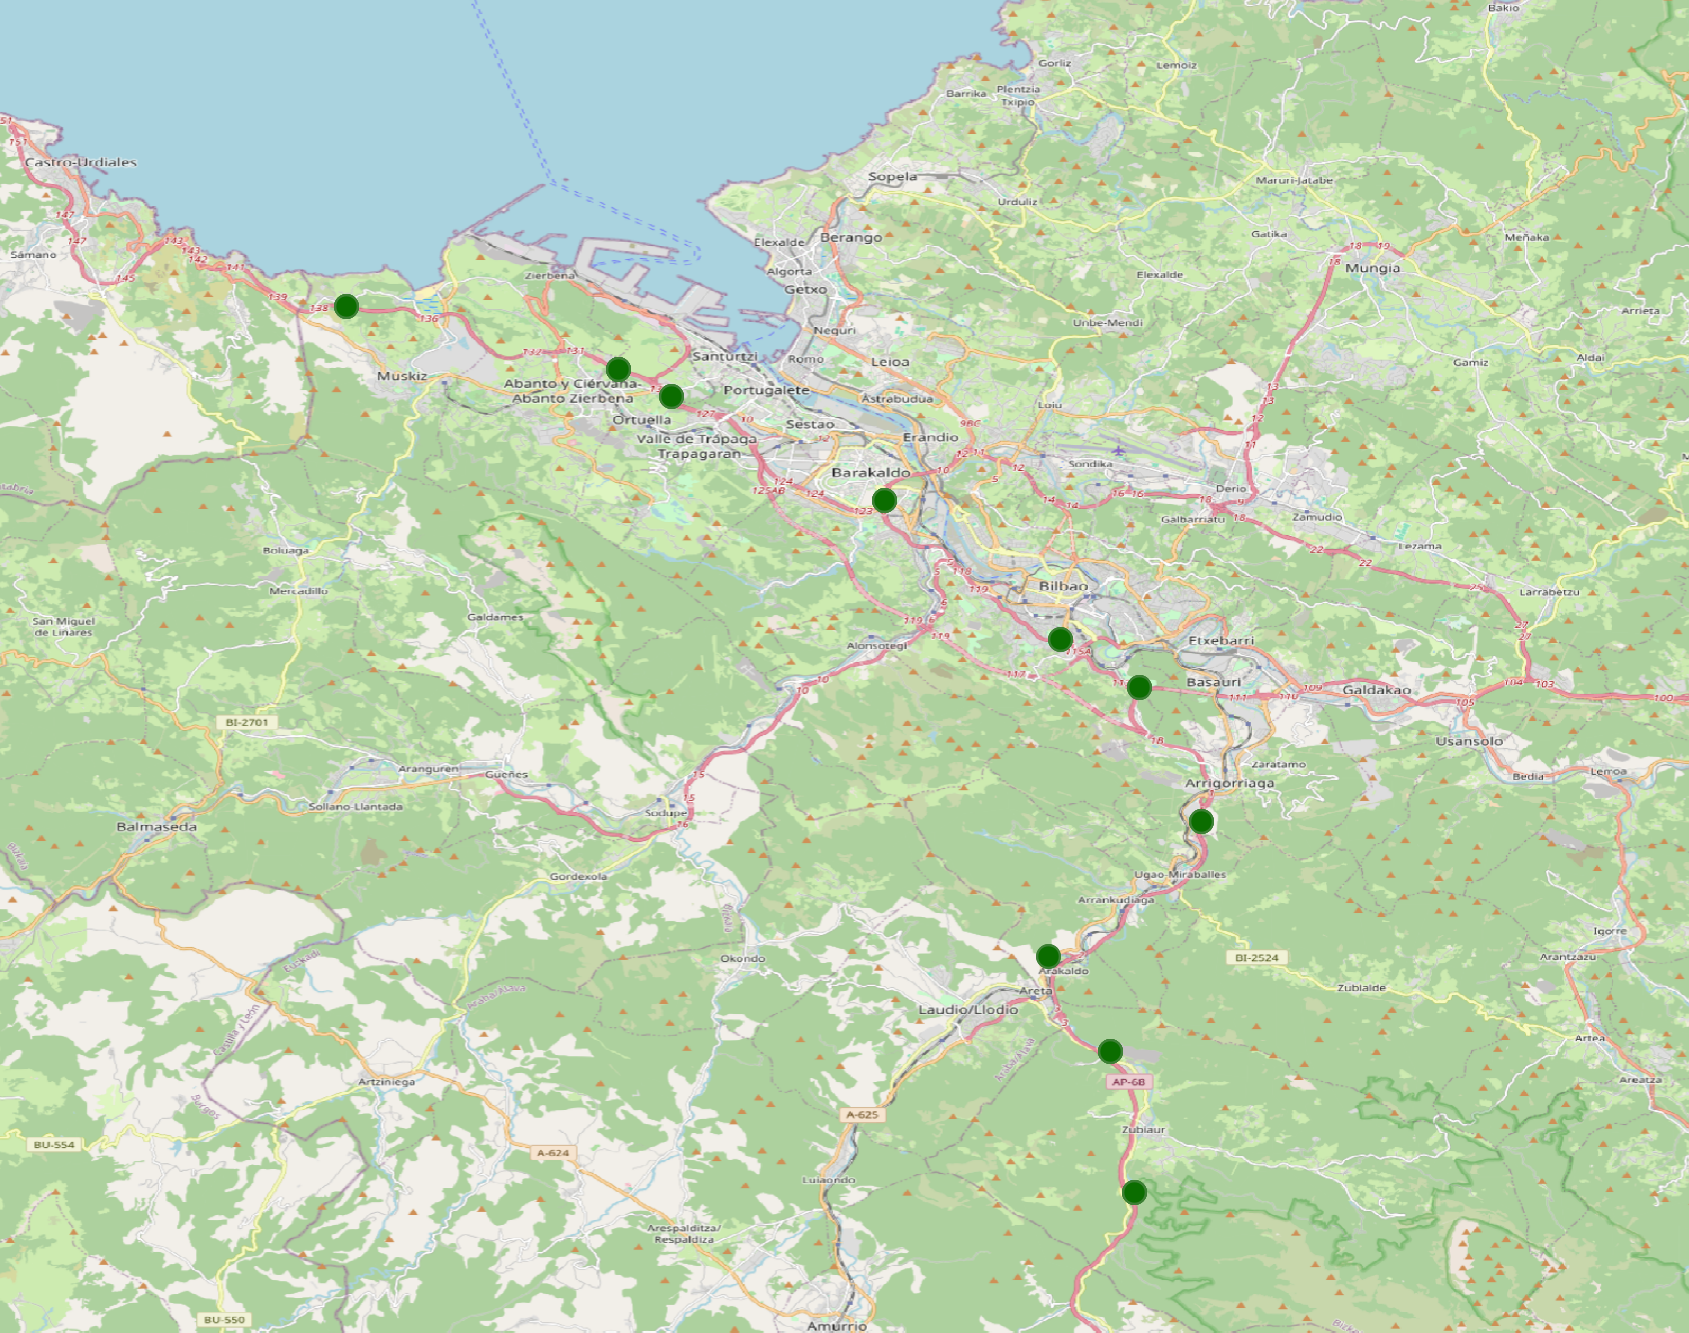
\includegraphics[width=0.65\textwidth]{includes/cap5/source_id_1_meters.png}
	\caption{Ubicación de aforos de la fuente Gobierno Vasco (source\_id = 1)}
	\label{fig:sourceid1_map}
\end{figure}

La Figura~\ref{fig:sourceid2_map} recoge la distribución de medidores correspondiente a la fuente \texttt{source\_id = 2} (Diputación Foral de Bizkaia). Esta fuente dispone de una extensa red de sensores desplegada a lo largo de la provincia, lo que proporciona una cobertura muy amplia y variada a nivel geográfico y funcional.

\begin{figure}[H]
	\centering
	\includegraphics[width=0.85\textwidth]{includes/cap5/source_id_2_meters.png}
	\caption{Ubicación de aforos de la fuente Diputación Foral de Bizkaia (source\_id = 2)}
	\label{fig:sourceid2_map}
\end{figure}

Finalmente, la Figura~\ref{fig:sourceid5_map} representa los sensores aportados por el \texttt{source\_id = 5} (Ayuntamiento de Bilbao), con presencia en los principales ejes viarios de la ciudad. Se conoce que existen más medidores instalados, pero el consistorio no ha habilitado su acceso público o no los tiene en funcionamiento, por razones que se desconocen.

\begin{figure}[H]
	\centering
	\includegraphics[width=0.85\textwidth]{includes/cap5/source_id_5_meters.png}
	\caption{Ubicación de aforos de la fuente Ayuntamiento de Bilbao (source\_id = 5)}
	\label{fig:sourceid5_map}
\end{figure}

Las incidencias se obtuvieron completamente para todos los sourceId.

En cuanto a la obtención de los datos meteorológicos, si bien es cierto que existe el API de meteorología del portal de Open Data del Gobierno Vasco \cite{apiMeteo}, éste presenta numerosos fallos a la hora de usarlo. Un claro ejemplo es la figura \ref{fig:euskalmet_api_error}. 

\begin{figure}[H]
	\centering
	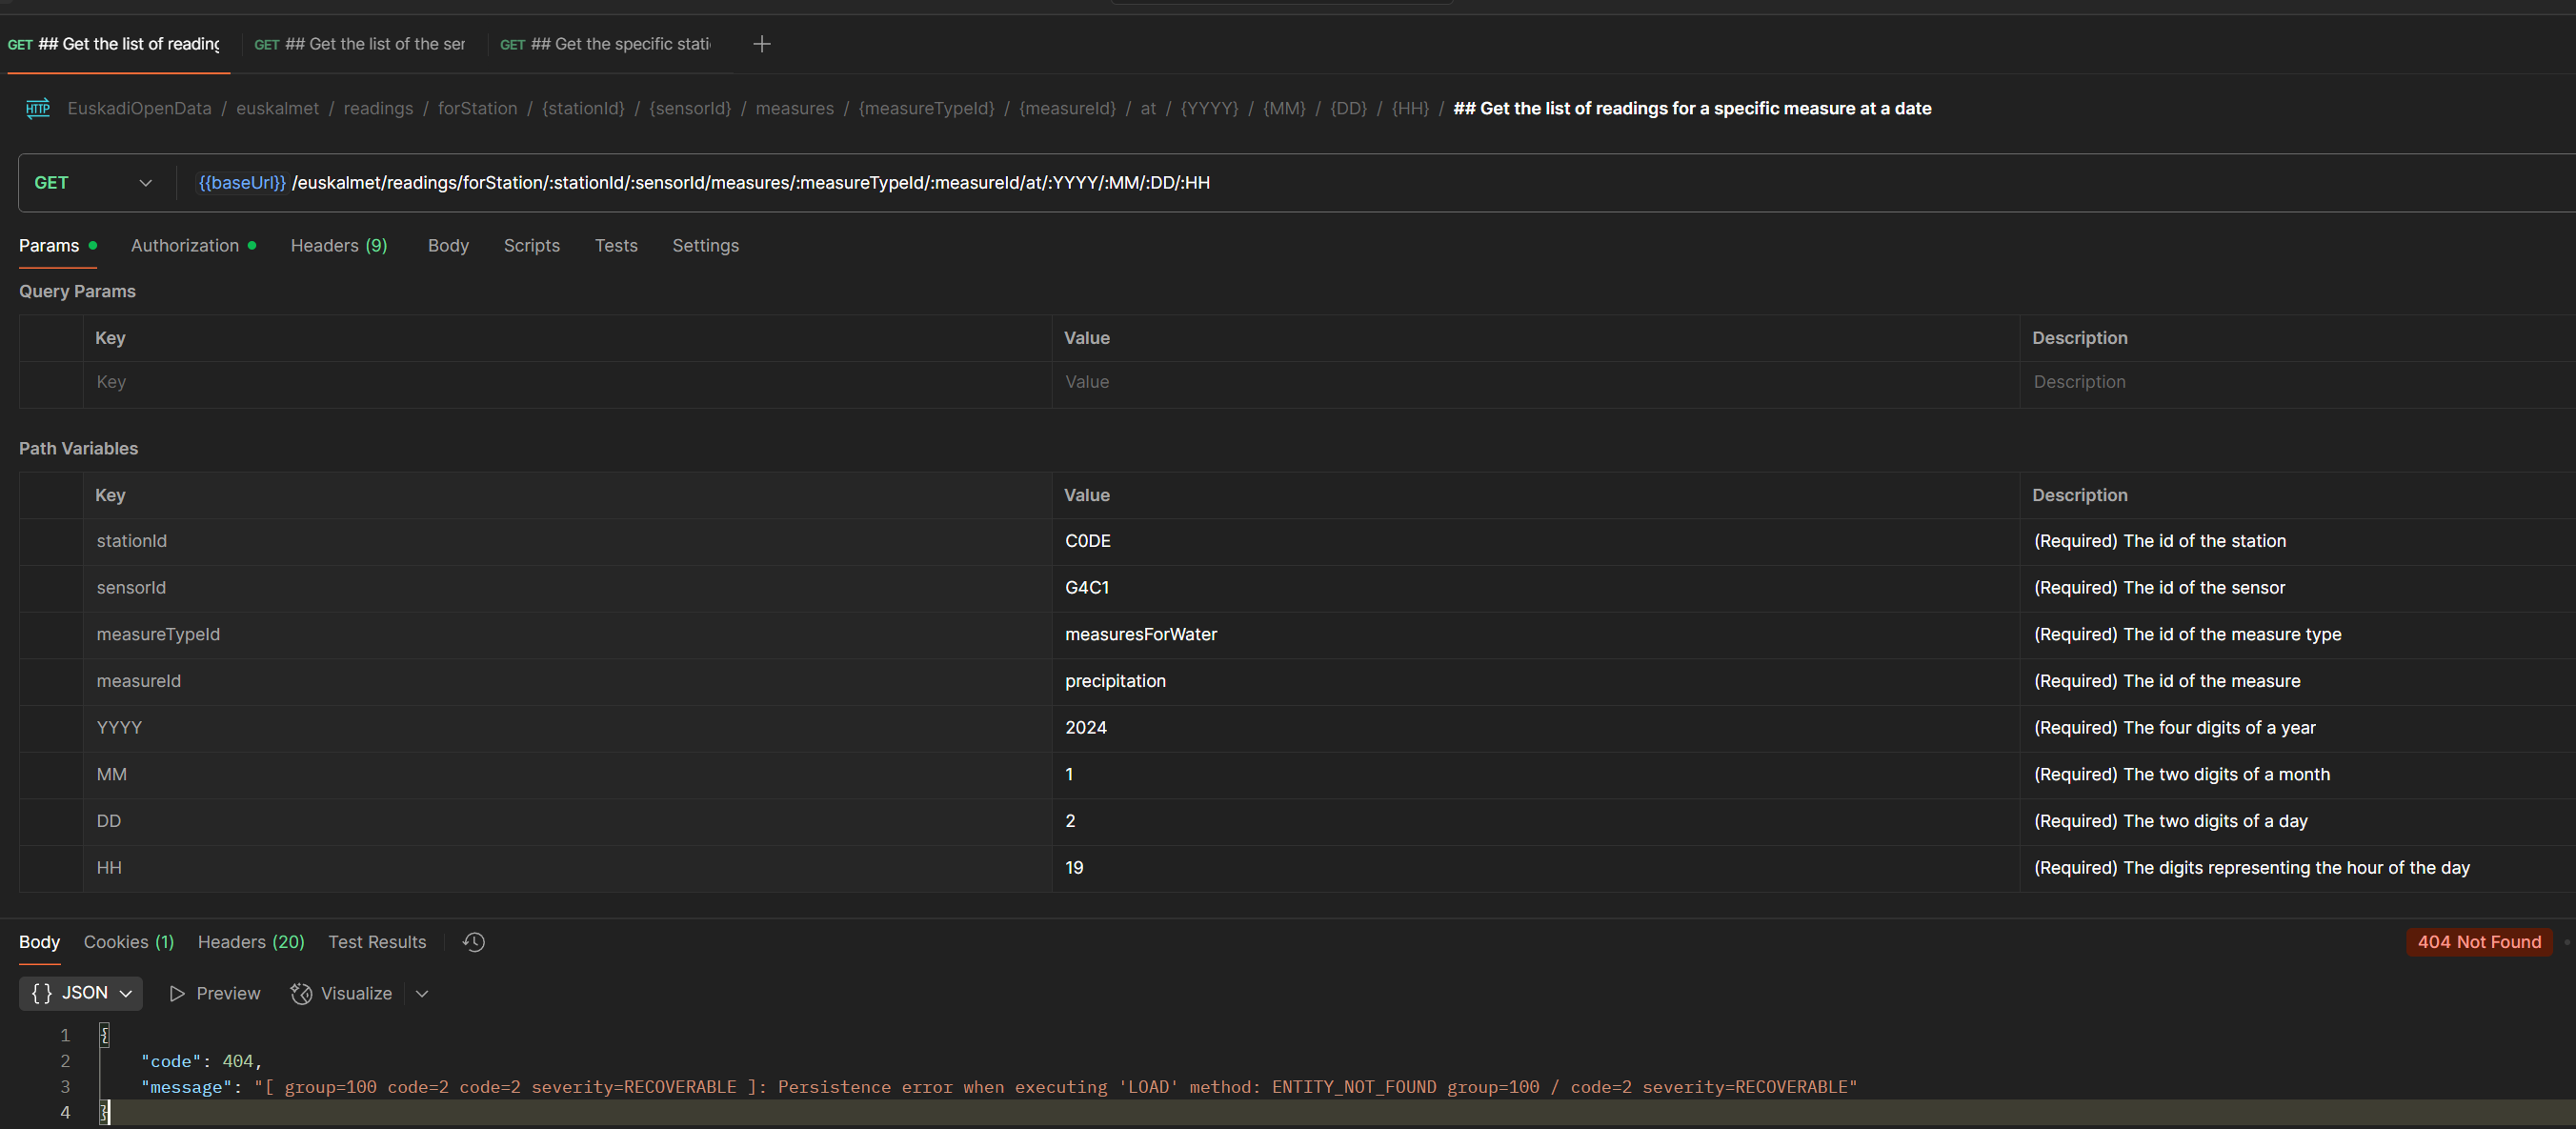
\includegraphics[width=0.95\textwidth]{includes/error_api_euskalmet.png}
	\caption{Ejemplo de error a la hora de consultar el API de Euskalmet.}
	\label{fig:euskalmet_api_error}
\end{figure}

Ante la incertidumbre sobre la calidad y disponibilidad de los datos inicialmente previstos, se exploraron alternativas para la obtención de información relevante. En este proceso, se identificó dentro del propio portal de Open Data del Gobierno Vasco un recurso adicional: las lecturas brutas recogidas por las estaciones meteorológicas correspondientes al año 2024, disponibles en formato XML y accesibles públicamente \cite{xmlMeteo2024}.

\subsubsection*{Modelo de datos almacenado}

Una vez explicadas las fuentes de datos, se podría comenzar a explicar cómo se van a almacenar dichos datos. En la figura \ref{fig:uml_classes} se puede ver las clases persistidas en la base de datos.

\begin{figure}[H]
	\centering
	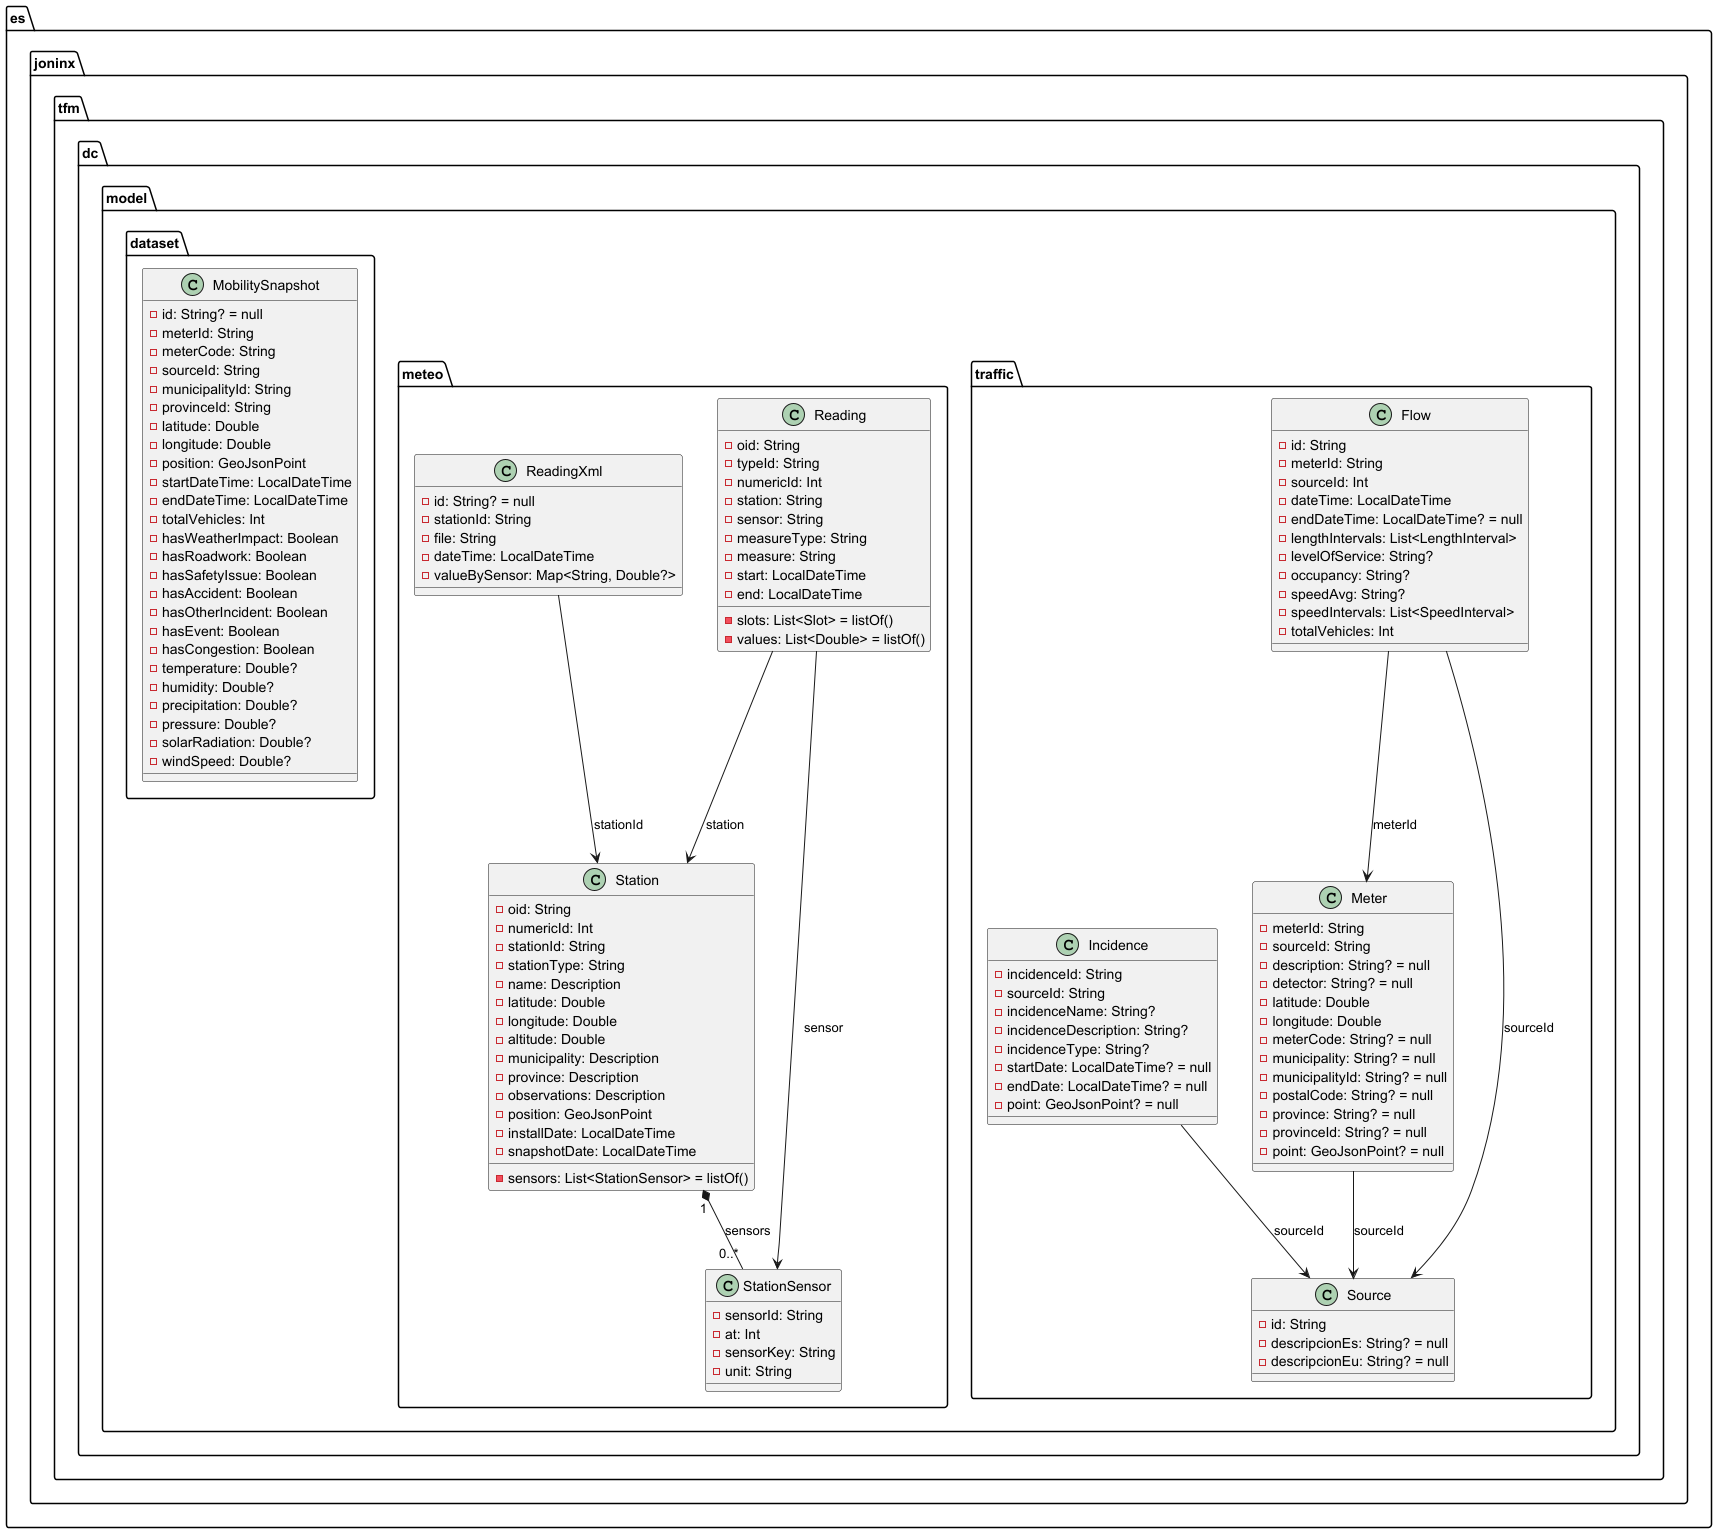
\includegraphics[width=0.95\textwidth]{includes/model_classes.png}
	\caption{Modelo de clases en UML de las entidades principales del sistema.}
	\label{fig:uml_classes}
\end{figure}

A continuación, se describen las entidades persistidas en base de datos, divididas por paquetes funcionales según su origen y propósito dentro del sistema: tráfico, meteorología y dataset resultante. Los datos de incidencias se incluyen dentro del paquete de tráfico, puesto que así viene encasillado en el API consultado. Cada clase representa un documento en la base de datos MongoDB, adaptado a una estructura flexible y orientada a documentos.

\paragraph*{Flow}
Representa una medición de flujo de tráfico captada por un aforador en una fecha y hora determinadas. Entre sus atributos destacan:
\begin{itemize}
	\item \texttt{id}: identificador único del registro.
	\item \texttt{meterId}: identificador del aforador que ha generado la medición.
	\item \texttt{sourceId}: origen de los datos (Gobierno Vasco, Ayuntamiento, etc.).
	\item \texttt{dateTime} y \texttt{endDateTIme}: marca temporal de la medición. Puede que la marca de final no esté informada.
	\item \texttt{totalVehicles}: número total de vehículos detectados.
	\item \texttt{speedAvg}: velocidades medias de los vehículos detectados.
	\item \texttt{lengthIntervals} y \texttt{speedIntervals}: listas de intervalos por longitudes y velocidades, útiles para análisis más detallados. No se usa en este caso de uso.
\end{itemize}

\paragraph*{Meter}
Contiene la información estática de los aforadores:
\begin{itemize}
	\item \texttt{meterId}, \texttt{sourceId}: identificadores del aforador y de la fuente de datos.
	\item \texttt{latitude}, \texttt{longitude} y \texttt{point}: ubicación geográfica. Útil el punto (tipo GeoJSON), puesto que es un índice geoespacial y se pueden realizar operaciones sobre el mismo (búsquedas por cercanía, distancias, etc).
	\item \texttt{postalCode}, \texttt{provinceId}, \texttt{municipalityId}: metadatos administrativos.
\end{itemize}

\paragraph*{Incidence}
Recoge información sobre incidencias viales que pueden afectar al tráfico:
\begin{itemize}
	\item \texttt{incidenceId}, \texttt{sourceId}: identificadores del evento y de la fuente de datos.
	\item \texttt{incidenceName} e \texttt{incidenceDescription}: información descriptiva textual de la incidencia.
	\item \texttt{incidenceType}, \texttt{incidenceLevel}: tipificación normalizada para su posterior uso como variable categórica.
	\item \texttt{cause}, \texttt{road}, \texttt{pkStart}, \texttt{pkEnd}, \texttt{cityTown}, \texttt{province}, \texttt{autonomousRegion}, \texttt{carRegistration}: información adicional de la incidencia. Recoge datos como la carretera, los puntos kilométricos de inicio y de fin e información administrativa. No se tratará en este caso de uso.
	\item \texttt{startDate}, \texttt{endDate}: intervalo de vigencia de la incidencia. Esta información es relevante.
	\item \texttt{point}: ubicación geoespacial (tipo GeoJSON). Útil para realizar búsquedas por cercanía.
\end{itemize}

\paragraph*{Source}
Representa los orígenes oficiales de datos, como el Gobierno Vasco o ayuntamientos. Sus campos identifican la organización y su descripción.

\vspace{1em}
\paragraph*{Reading}
Es la clase principal para representar una lectura meteorológica horaria del API. Sin embargo, no se ha usado esta entidad para construir el dataset.
\begin{itemize}
	\item \texttt{oid}: identificador de la lectura.
	\item \texttt{typeId}: tipo de la lectura.
	\item \texttt{station}: estación meteorológica emisora.
	\item \texttt{sensor}: sensor responsable de la medición (\texttt{StationSensor}).
	\item \texttt{measureType} y \texttt{measure}: categorización de la medición.
	\item \texttt{start}, \texttt{end}: momento para el cual se ha realizado la medición.
	\item \texttt{slots}, \texttt{values}: forma en la que tiene el API de almacenar las mediciones. Cada elemento del slot se corresponde a un elemento de values, en la misma posición, indicando lo que se mide y su valor.
\end{itemize}

\paragraph*{ReadingXml}
Clase específica para lecturas meteorológicas históricas extraídas desde ficheros XML. A diferencia de \texttt{Reading}, puede contener estructuras agrupadas por múltiples sensores. Es la clase definitiva empleada para construir el dataset.
\begin{itemize}
	\item \texttt{id}: identificador de la lectura.
	\item \texttt{stationId}: identificador de la estación meteorológica de la lectura.
	\item \texttt{file}: fichero de donde se ha extraído el dato de medición.
	\item \texttt{dateTime}: momento para el cual se ha realizado la medición.
	\item \texttt{valueBySensor}: forma en la que se almacenan las mediciones. El elemento clave identifica el tipo de medición y el valor indica el valor propio de la medición.
\end{itemize}

\paragraph*{Station}
Define las estaciones meteorológicas que proporcionan las lecturas:
\begin{itemize}
	\item \texttt{stationId}: identificador único de la estación de medición.
	\item \texttt{name}, \texttt{municipality}, \texttt{province}: información administrativa.
	\item \texttt{latitude}, \texttt{longitude}, \texttt{altitude} y \texttt{position}: coordenadas geográficas.
	\item \texttt{sensors}: lista de sensores instalados.
\end{itemize}

\paragraph*{StationSensor}
Define la configuración física de un sensor en una estación:
\begin{itemize}
	\item \texttt{sensorId}, \texttt{sensorKey}: clave de sensor y código técnico.
	\item \texttt{unit}, \texttt{at}: unidad de medida y altura del sensor (en centímetros).
\end{itemize}

\vspace{1em}
\paragraph*{MobilitySnapshot}
Es la entidad clave que representa un punto de datos enriquecido para el modelo predictivo. Cada snapshot incluye:
\begin{itemize}
	\item \texttt{id}: identificador único del dato.
	\item \texttt{meterId}, \texttt{meterCode}: información identificativa del aforador del cual se ha extraído la información de Flow.
	\item \texttt{totalVehicles}: indica la cantidad de vehículos que han pasado por este punto entre en el espacio temporal definido.
	\item \texttt{latitude}, \texttt{longitude}, \texttt{position}: información geoespacial del snapshot. Nótese que el campo positión es de tipo GeoJson.
	\item \texttt{startDateTime}, \texttt{endDateTime}: indica entre qué momentos es válido este snapshot.
	\item \texttt{hasAccident}, \texttt{hasWeatherImpact}, \texttt{hasConstruction}, etc: indica si durante este espacio temporal cerca de este punto ha ocurrido alguna incidencia del tipo.
	\item \texttt{temperature}, \texttt{humidity}, \texttt{windSpeed}, \texttt{solarRadiation}, \texttt{pressure}, etc: indica los valores meteorológicos del propio snapshot.
\end{itemize}

Esta clase es el resultado final del proceso de integración de datos y constituye la base sobre la que se entrena el modelo de predicción de tráfico.

\subsection{Recolección, arquitectura y patrones de diseño empleados}

El software encargado de la recolección de datos se ha desarrollado en \textbf{Kotlin con Spring Boot}, aplicando principios de arquitectura hexagonal y múltiples patrones de diseño para garantizar su mantenibilidad y robustez. Entre los patrones de diseño empleados destacan: \gls{design_pattern:builder}, \gls{design_pattern:repository}, \gls{design_pattern:servicelayer}, \gls{design_pattern:dto}, \gls{design_pattern:helper_utility}, \gls{design_pattern:facade} y \gls{design_pattern:factory_singleton}.

El sistema de integración y procesamiento de datos ha sido desarrollado en Kotlin, un lenguaje moderno que combina características orientadas a objetos y funcionales. La clase \texttt{MobilitySnapshotGeneratorService}, pieza central del sistema, hace uso de varias construcciones idiomáticas que representan buenas prácticas del lenguaje y potencian la expresividad, la seguridad y la eficiencia en tiempo de desarrollo.

A continuación se destacan las características más reseñables del uso de Kotlin en dicha implementación:

\begin{itemize}
	\item \textbf{Inferencia de tipos}: permite declarar variables sin especificar explícitamente su tipo cuando este es deducible por el compilador, lo que mejora la legibilidad. Por ejemplo:
	\begin{lstlisting}[language=Kotlin]
		val intervals = mutableListOf<Pair<LocalDateTime, LocalDateTime>>()
	\end{lstlisting}
	
	\item \textbf{Funciones de orden superior y operadores de colección}: se hace uso extensivo de funciones como \texttt{mapNotNull}, \texttt{groupBy}, \texttt{sumOf}, y \texttt{forEachIndexed}, lo que refleja el paradigma funcional del lenguaje.
	\begin{lstlisting}[language=Kotlin]
		val groupedByMeter = flows.groupBy { it.meterId }
		val snapshots = groupedByMeter.mapNotNull { (meterId, flowList) -> ... }
	\end{lstlisting}
	
	\item \textbf{Acceso seguro a valores opcionales con \texttt{let}}: se utiliza para gestionar accesos a valores almacenados en cachés evitando estructuras condicionales explícitas.
	\begin{lstlisting}[language=Kotlin]
		meterToStationCache[meterId]?.let {
			log.debug("Cache HIT: meterId=$meterId → stationId=$it")
			return it
		}
	\end{lstlisting}
	
	\item \textbf{Operador Elvis (\texttt{?:})}: permite proporcionar valores por defecto ante posibles nulos, mejorando la seguridad frente a \texttt{NullPointerException}.
	\begin{lstlisting}[language=Kotlin]
		val meters = meterRepository.findAllBySourceIdIn(sourceIds)
		.collectMap { it.meterId }
		.block() ?: emptyMap()
	\end{lstlisting}
	
	\item \textbf{Lambdas expresivas y destructuración de pares}: se utilizan para recorrer colecciones de forma clara, aprovechando las capacidades de Kotlin para trabajar con estructuras complejas.
	\begin{lstlisting}[language=Kotlin]
		intervals.forEachIndexed { idx, (intervalStart, intervalEnd) -> ... }
	\end{lstlisting}
	
	\item \textbf{Inyección de dependencias vía constructor}: siguiendo los principios de inversión de dependencias (en otras palabras, un término que mezcla los conceptos de Inyección de Dependencias e Inversión de Control), se definen todos los componentes del servicio a través del constructor primario.
	\begin{lstlisting}[language=Kotlin]
		class MobilitySnapshotGeneratorService(
		private val cfg: Cfg,
		private val snapshotBuilder: MobilitySnapshotBuilder,
		...
		)
	\end{lstlisting}
	
	\item \textbf{Uso de \texttt{companion object} para logging}: se emplea una instancia estática del logger utilizando el enfoque idiomático del lenguaje.
	\begin{lstlisting}[language=Kotlin]
		companion object {
			val log: Logger = LogManager.getLogger(this::class.java)
		}
	\end{lstlisting}
	
	\item \textbf{Uso responsable de colecciones mutables}: aunque se utilizan listas mutables para la generación de intervalos y resultados temporales, estas estructuras se manejan de forma controlada y local, siguiendo las recomendaciones del lenguaje.
\end{itemize}

El uso de estas características idiomáticas refleja una implementación robusta, alineada con las buenas prácticas modernas del ecosistema Kotlin, y facilita tanto el mantenimiento del código como su extensibilidad futura.

La decisión de utilizar una base de datos \textbf{NoSQL, MongoDB}, responde a la necesidad de trabajar con estructuras flexibles, heterogéneas y de gran volumen, propias del contexto del proyecto.

\subsection{Decisiones de construcción del dataset}

Tras la integración de las fuentes de datos de tráfico, meteorología e incidencias, se llevó a cabo un proceso de análisis y consolidación de información para la construcción del dataset final utilizado por el modelo de predicción. Este dataset, modelado a través de la clase \texttt{MobilitySnapshot}, resume en cada observación todos los factores que pueden influir en la intensidad del tráfico en un instante y ubicación concretos. En los siguientes apartados se detallan las decisiones tomadas en relación con cada fuente de información, comenzando por la tipificación de incidencias viales.

\subsubsection*{Obtención y estructuración de incidencias}
% Si ponemos así no se imprime en el indice
%\subsubsection*{Obtención y estructuración de incidencias}

A partir del análisis exploratorio de las incidencias disponibles en la base de datos, se identificaron distintos tipos reportados a lo largo del tiempo por las diferentes entidades públicas. La tabla \ref{tab:incidencias_frecuencia} resume las categorías encontradas, junto con su frecuencia absoluta. Es importante tener en cuenta que estos datos corresponden a toda la \acrshort{capv}, no solo a Bizkaia.

\begin{table}[H]
	\centering
	\small
	\caption{Frecuencia de incidencias por tipo original}
	\label{tab:incidencias_frecuencia}
	\begin{tabularx}{\textwidth}{rX}
		\toprule
		\textbf{Frecuencia} & \textbf{Tipo de incidencia} \\
		\midrule
		41792 & Puertos de montaña \\
		8544  & Obras \\
		8391  & Vialidad invernal tramos \\
		7594  & Seguridad vial \\
		3155  & Accidente \\
		2005  & Otras incidencias \\
		203   & Meteorológica \\
		165   & OTRO \\
		135   & OBRA \\
		78    & EVEN \\
		3     & Retención \\
		\bottomrule
	\end{tabularx}
\end{table}

Con base en esta información, se procedió a una consolidación tipológica siguiendo tres criterios principales:

\begin{itemize}
	\item Evitar la existencia de categorías con muy baja frecuencia.
	\item Unificar variantes ortográficas o nomenclaturas inconsistentes (por ejemplo, \texttt{Obras} y \texttt{OBRA}).
	\item Mantener las categorías que aportan valor explicativo al modelo de predicción.
\end{itemize}

El resultado es una agrupación validada que se resume en la tabla \ref{tab:agrupacion_incidencias}.

\begin{table}[H]
	\centering
	\small
	\caption{Agrupación final de incidencias para el modelo predictivo}
	\label{tab:agrupacion_incidencias}
	\begin{comment}\renewcommand{\arraystretch}{1.3}\end{comment}
	\begin{tabularx}{\textwidth}{lXrX}
		\toprule
		\textbf{Categoría general} & \textbf{Tipos incluidos} & \textbf{Total casos} & \textbf{Variable sugerida} \\
		\midrule
		\texttt{WEATHER}    & Puertos de montaña, Vialidad invernal tramos, Meteorológica & \textbf{50.386} & \texttt{hasWeatherImpact} \\
		\texttt{ROADWORK}   & Obras, OBRA                                                  & \textbf{8.679}  & \texttt{hasRoadwork} \\
		\texttt{SAFETY}     & Seguridad vial                                               & \textbf{7.594}  & \texttt{hasSafetyIssue} \\
		\texttt{ACCIDENT}   & Accidente                                                    & \textbf{3.155}  & \texttt{hasAccident} \\
		\texttt{OTHER}      & Otras incidencias, OTRO                                      & \textbf{2.170}  & \texttt{hasOtherIncident} \\
		\texttt{EVENT}      & EVEN                                                         & \textbf{78}     & \texttt{hasEvent} \\
		\texttt{CONGESTION} & Retención                                                    & \textbf{3}      & \texttt{hasCongestion} \\
		\bottomrule
	\end{tabularx}
\end{table}

Las variables anteriores se incorporan al dataset como flags booleanos en la clase \texttt{MobilitySnapshot}, permitiendo representar si una incidencia de dicha categoría estaba activa o no en el momento de cada observación. Las variables mínimas propuestas son:

\begin{lstlisting}[language=Kotlin, caption={Variables mínimas de incidencias en MobilitySnapshot}]
	val hasWeatherImpact: Boolean
	val hasRoadwork: Boolean
	val hasSafetyIssue: Boolean
	val hasAccident: Boolean
	val hasOtherIncident: Boolean
\end{lstlisting}

Adicionalmente, y si el volumen de datos lo justifica en futuras versiones del dataset, se podrían incorporar:

\begin{lstlisting}[language=Kotlin, caption={Variables opcionales}]
	val hasEvent: Boolean
	val hasCongestion: Boolean
\end{lstlisting}

\subsubsection*{Selección e integración de variables meteorológicas}

El sistema de captación meteorológica empleado en este proyecto incluye un conjunto amplio y heterogéneo de sensores distribuidos en estaciones automáticas de observación repartidas por la CAPV. Cada estación contiene múltiples sensores, y cada sensor puede registrar una variable distinta a una altura determinada del suelo (por ejemplo, 0 cm, 1050 cm o 2200 cm). 

Como se detalla en el \hyperref[anexo:sensores]{Anexo~B}, se dispone de un amplio conjunto de sensores meteorológicos, cada uno con una codificación propia y una descripción técnica. En concreto, se incluyen más de 30 tipos distintos de sensores, desde condiciones atmosféricas hasta mediciones marinas o subterráneas. Algunos ejemplos de variables disponibles son: temperatura del aire (\texttt{Tem.Aire}), humedad relativa (\texttt{Humedad}), radiación solar (\texttt{Irradia.}), presión atmosférica (\texttt{Presión}), dirección del viento (\texttt{Dir.Med.}), visibilidad, y muchas otras relacionadas con agua o condiciones marítimas. 

Dado el objetivo de este proyecto es predecir el flujo de tráfico urbano, se realizó una \textbf{selección cuidadosa de las variables meteorológicas más relevantes}, descartando aquellas que, por su naturaleza o localización (ej. marítimas), no presentaban una influencia directa sobre la movilidad terrestre urbana.

Las variables seleccionadas, junto con su justificación práctica, se muestran en la tabla \ref{tab:seleccion_meteo}.

\begin{table}[H]
	\centering
	\small
	\caption{Selección de sensores meteorológicos y su relevancia para la predicción de tráfico}
	\label{tab:seleccion_meteo}
	\begin{comment}\renewcommand{\arraystretch}{1.3}\end{comment}
	\begin{tabularx}{\textwidth}{l l X}
		\toprule
		\textbf{Categoría} & \textbf{SensorKey base} & \textbf{Justificación} \\
		\midrule
		Temperatura del aire & \texttt{Tem\_Aire\_\_a\_*} & Influye en el comportamiento de conducción y el volumen de tráfico. \\
		Humedad relativa & \texttt{Humedad\_\_a\_*} & Afecta la visibilidad y adherencia de los neumáticos. \\
		Precipitación acumulada & \texttt{Precip\_\_\_a\_*} & Altamente correlacionada con congestiones y reducción de velocidad. \\
		Presión atmosférica & \texttt{Presion\_\_a\_*} & Indicador indirecto de cambios climáticos significativos. \\
		Radiación solar & \texttt{Irradia\_\_\_a\_*} & Relacionada con condiciones extremas de iluminación y temperatura. \\
		Velocidad media del viento & \texttt{Vel\_Med\_\_a\_*} & Indicador de fenómenos meteorológicos adversos (rachas, tormentas). \\
		\bottomrule
	\end{tabularx}
\end{table}

Para cada una de estas categorías, se escoge \textbf{el sensor más representativo o más cercano al suelo} disponible en cada estación. Este criterio asegura la mayor homogeneidad entre estaciones y la mayor cercanía posible a las condiciones experimentadas en carretera.

Finalmente, estas variables se integran dentro de cada observación del dataset final mediante su asociación espacio-temporal al flujo de tráfico correspondiente, quedando reflejadas como campos meteorológicos en la clase \texttt{MobilitySnapshot}:

\begin{lstlisting}[language=Kotlin, caption={Variables meteorológicas integradas en MobilitySnapshot}]
	val temperature: Double?
	val humidity: Double?
	val precipitation: Double?
	val pressure: Double?
	val solarRadiation: Double?
	val windSpeed: Double?
\end{lstlisting}

Estas variables permiten modelar de forma efectiva el efecto de las condiciones meteorológicas sobre la movilidad urbana, mejorando la capacidad predictiva del modelo de aprendizaje profundo.

\subsubsection*{Fusión e integración: la clase \texttt{MobilitySnapshot}}

La entidad central para la construcción del dataset es la clase \texttt{MobilitySnapshot}, que representa un registro aglutinado por instante temporal y ubicación, integrando la información de:

\begin{itemize}
	\item \textbf{Flujos de tráfico (\texttt{Flow})}: variables como \texttt{meterId}, \texttt{dateTime}, \texttt{totalVehicles}, y metadatos geográficos.
	\item \textbf{Meteorología (\texttt{Reading})}: valores de los sensores seleccionados asociados espacial y temporalmente al flujo.
	\item \textbf{Incidencias (\texttt{Incidence})}: información de incidencias activas cercanas en tiempo y espacio, codificadas según la tipología definida.
\end{itemize}

El proceso de generación de las observaciones enriquecidas se implementa en el servicio \texttt{MobilitySnapshotGeneratorService}, dentro del método \texttt{generateSnapshots()}. Este método ejecuta de forma secuencial la construcción de objetos \texttt{MobilitySnapshot}, cada uno de los cuales encapsula una observación consolidada de movilidad para un instante y punto geográfico concretos. La lógica está diseñada para ser robusta y escalable, gestionando datos de múltiples fuentes (flujos, meteorología e incidencias) mediante el uso de procesamiento por intervalos y agrupación por sensor.

El flujo completo queda representado en la Figura \ref{fig:sequence_mobility_snapshot}, mediante un diagrama de secuencia UML, que ilustra claramente el intercambio entre repositorios, lógica de negocio y servicios de persistencia.

\begin{figure}[H]
	\centering
	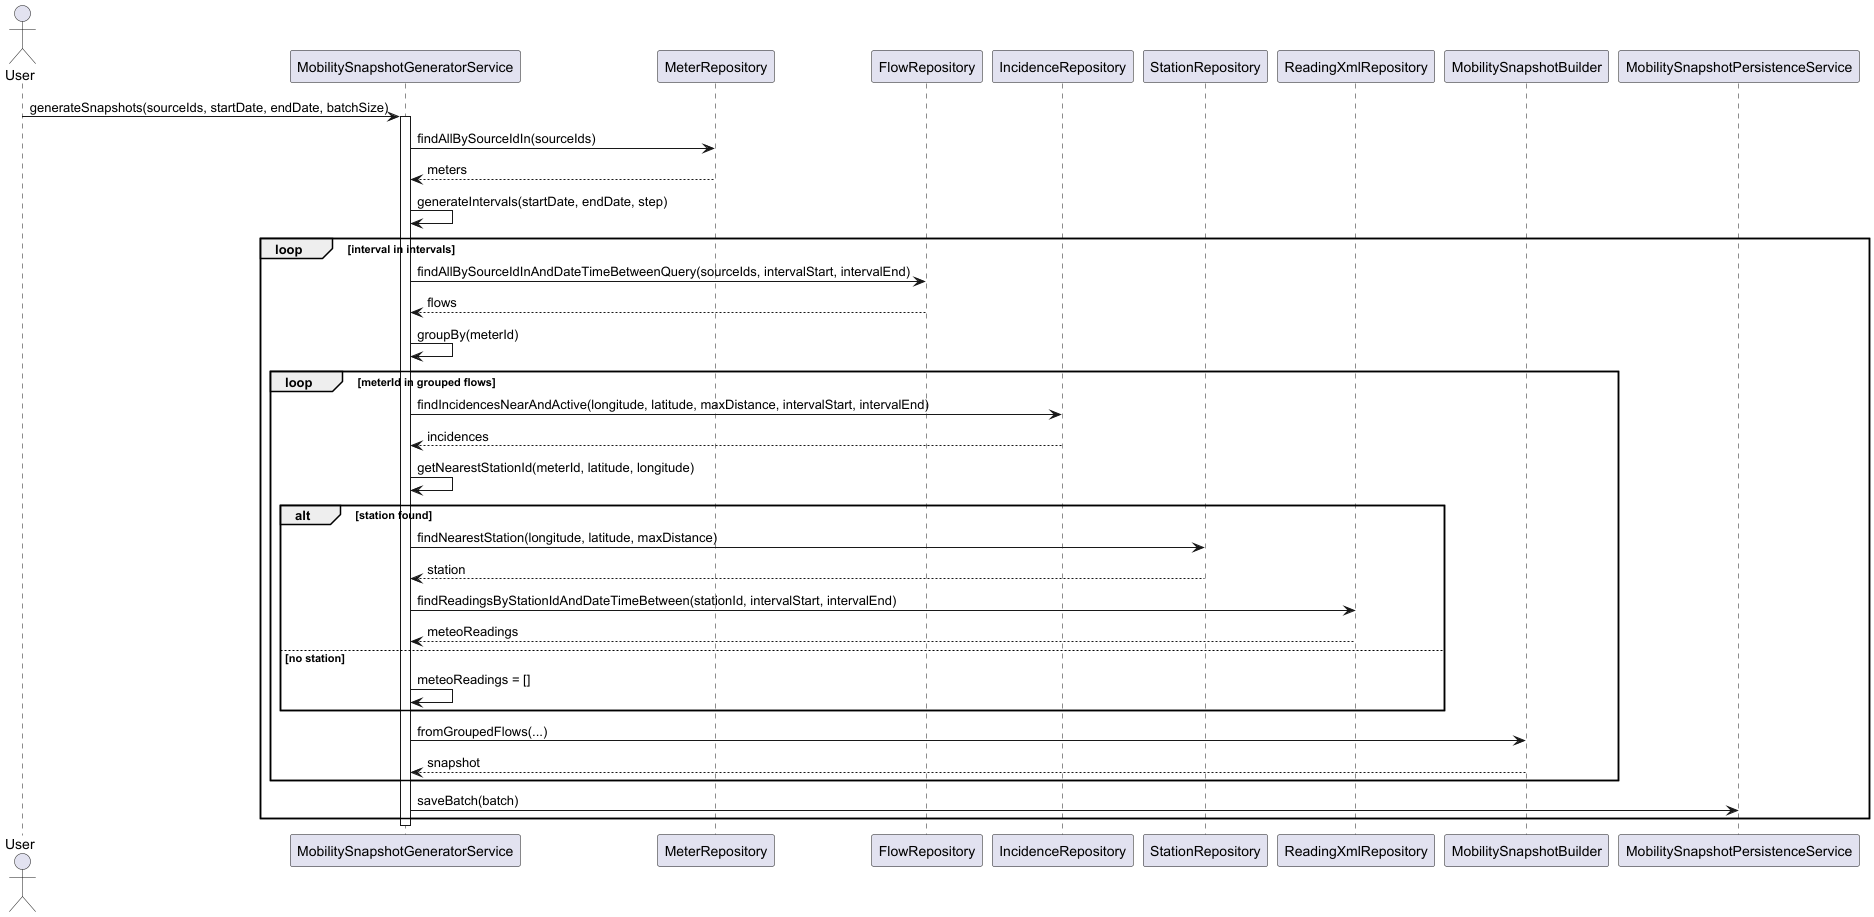
\includegraphics[width=0.95\textwidth]{includes/snapshot_generator_sequence.png}
	\caption{Diagrama de secuencia de integración y persistencia en \texttt{MobilitySnapshot}.}
	\label{fig:sequence_mobility_snapshot}
\end{figure}

El código fuente completo del componente encargado de llevar a cabo esta integración puede consultarse en el \hyperref[anexo:snapshot_generator]{Anexo~C}, donde se incluye la clase \texttt{MobilitySnapshotGeneratorService} desarrollada específicamente para este propósito.

El proceso se puede descomponer en los siguientes pasos:

\begin{enumerate}
	\item \textbf{Inicialización:} se obtienen todos los aforadores activos (\texttt{Meter}) correspondientes a los identificadores de fuente (\texttt{sourceIds}) indicados.
	\item \textbf{Ventanas temporales:} se generan intervalos de tiempo equiespaciados de 30 minutos entre las fechas de inicio y fin.
	\item \textbf{Extracción de flujos:} para cada intervalo, se recuperan todos los flujos de vehículos (\texttt{Flow}) registrados en ese rango temporal y se agrupan por aforador (\texttt{meterId}).
	\item \textbf{Procesamiento por aforador:} para cada grupo de flujos:
	\begin{itemize}
		\item Se localiza el aforador correspondiente y se calcula el número total de vehículos en la ventana.
		\item Se consultan las incidencias viales (\texttt{Incidence}) activas y geoespacialmente cercanas (500 metros) en el intervalo.
		\item Se determina la estación meteorológica más cercana usando una cache interna. Si existe, se recuperan las lecturas (\texttt{Reading}) correspondientes al intervalo temporal.
	\end{itemize}
	\item \textbf{Construcción del snapshot:} con todos los datos anteriores, se construye el objeto \texttt{MobilitySnapshot} mediante el \texttt{MobilitySnapshotBuilder}.
	\item \textbf{Persistencia por lotes:} los snapshots generados se agrupan en bloques de tamaño configurable (por defecto 500) y se guardan en la base de datos de forma transaccional.
\end{enumerate}

Para procesar los datos por ventanas temporales consecutivas, se implementa una función utilitaria llamada \texttt{generateIntervals()}, que permite dividir un periodo de tiempo en subintervalos de duración fija. Este procedimiento es fundamental en el procesamiento de datos temporales y en la agregación de observaciones como \texttt{MobilitySnapshot}.

El algoritmo se describe de la siguiente forma.

\vspace{1em}
\noindent \textbf{Descripción del funcionamiento:}
\begin{itemize}
	\item La función recibe un instante inicial (\texttt{start}), un instante final (\texttt{end}) y una duración fija (\texttt{step}).
	\item Crea una lista vacía de intervalos temporales.
	\item Mediante un bucle, se van generando pares de fechas consecutivos, avanzando de \texttt{step} en \texttt{step}.
	\item Si el último intervalo excede el tiempo final, se ajusta automáticamente para que el límite superior sea exactamente \texttt{end}.
	\item Devuelve la lista completa de intervalos como pares de fechas (\texttt{Pair<start, end>}).
\end{itemize}

\vspace{1em}
\noindent \textbf{Ejemplo práctico:}
\begin{lstlisting}[language=Kotlin, caption={Ejemplo de uso con intervalos de 30 minutos}]
	generateIntervals(start = 2024-01-01T00:00, end = 2024-01-01T01:00, step = Duration.ofMinutes(30))
\end{lstlisting}

\noindent El resultado de este ejemplo sería:
\begin{verbatim}
	[ (2024-01-01T00:00, 2024-01-01T00:30), (2024-01-01T00:30, 2024-01-01T01:00) ]
\end{verbatim}

Este mecanismo permite particionar grandes volúmenes de datos históricos en unidades manejables, facilitando la agregación de información por tramos y reduciendo la carga computacional de los algoritmos de predicción.

Este proceso se ejecuta para todas las ventanas temporales dentro del periodo solicitado, permitiendo cubrir días, semanas o incluso meses de observaciones. Se emplean caches internas y colecciones reactivas para optimizar el rendimiento del sistema y permitir el escalado.

\subsubsection*{Consideraciones finales para la generación del dataset}

Una decisión fundamental en la construcción del dataset es la selección del intervalo temporal con el que se van a agrupar las observaciones. Este proceso, conocido como \textit{resampling temporal}, consiste en consolidar las mediciones de tráfico (\texttt{Flow}) en tramos de tiempo consecutivos y homogéneos. Esta práctica es común en el análisis de series temporales y presenta múltiples ventajas:

\begin{itemize}
	\item \textbf{Reducción de dispersión:} ayuda a evitar huecos en las series temporales, suavizando el ruido y mejorando la capacidad de generalización del modelo.
	\item \textbf{Homogeneización del dataset:} garantiza que todas las observaciones estén espaciadas en el tiempo con la misma frecuencia, lo cual es esencial para el entrenamiento supervisado.
	\item \textbf{Facilitación de integración con otras fuentes:} permite alinear los flujos con los datos meteorológicos e incidencias, los cuales pueden tener frecuencias distintas o menos regulares.
	\item \textbf{Reducción de volumen de datos:} disminuye la cantidad de registros generados, lo que mejora la eficiencia tanto en almacenamiento como en entrenamiento de modelos.
\end{itemize}

\vspace{1em}
\noindent La elección del intervalo temporal óptimo depende del equilibrio entre granularidad, capacidad computacional y riqueza informativa. Las alternativas más comunes son:

\begin{itemize}
	\item \textbf{Intervalos de 1 hora:} proporcionan una agregación suficiente para análisis diarios o semanales, son compatibles con muchos datasets públicos, pero pueden enmascarar variaciones de corto plazo (como retenciones puntuales).
	
	\item \textbf{Intervalos de 30 minutos:} capturan mejor los picos de tráfico y permiten reflejar dinámicas más rápidas (por ejemplo, alteraciones por accidentes o climatología adversa). Este intervalo ha sido el seleccionado en este proyecto como punto de partida, ya que ofrece un buen compromiso entre granularidad y manejabilidad.
	
	\item \textbf{Intervalos de 15 minutos o menos:} pueden resultar útiles si se dispone de datos de alta frecuencia, pero también pueden introducir más ruido o generar datasets demasiado voluminosos para ciertos entornos de cómputo.
\end{itemize}

\begin{table}[H]
	\centering
	\small
	\caption{Comparativa entre intervalos temporales posibles para el resampling}
	\label{tab:resample_comparison}
	\begin{comment}\renewcommand{\arraystretch}{1.4}\end{comment}
	\begin{tabularx}{\textwidth}{lXXX}
		\toprule
		\textbf{Criterio} & \textbf{15 minutos} & \textbf{30 minutos} & \textbf{1 hora} \\
		\midrule
		\textbf{Granularidad} & Alta & Media & Baja \\
		\textbf{Captura de picos} & Muy buena & Buena & Limitada \\
		\textbf{Volumen de datos} & Alto & Medio & Bajo \\
		\textbf{Riesgo de ruido} & Alto & Bajo-Medio & Bajo \\
		\textbf{Compatibilidad con fuentes externas} & Menor & Alta & Alta \\
		\textbf{Recomendado para} &
		Predicción muy reactiva o microanálisis &
		Equilibrio general &
		Análisis macro o planificación \\
		\bottomrule
	\end{tabularx}
\end{table}

En la Tabla \ref{tab:resample_comparison} se puede apreciar resumidamente las consideraciones descritas anteriormente.

\vspace{1em}
\noindent \textbf{Decisión tomada:} el sistema desarrollado trabaja por defecto con ventanas de \textbf{30 minutos}. Esta elección permite capturar transiciones relevantes en la movilidad sin incrementar en exceso la complejidad del dataset. No obstante, la arquitectura del generador (\texttt{MobilitySnapshotGeneratorService}) permite modificar este parámetro fácilmente para experimentar con alternativas. Por ejemplo:

\begin{itemize}
	\item Reducir a 15 minutos si se observan patrones planos o poca sensibilidad a eventos puntuales.
	\item Aumentar a 1 hora si el volumen de datos es demasiado elevado o si se prioriza una vista agregada del tráfico.
\end{itemize}

\subsection{Arquitectura y pipeline general del proyecto}

A continuación, se presenta una descripción completa de la arquitectura y el pipeline diseñado para este proyecto, abarcando desde la recolección inicial de datos hasta la generación y validación de modelos predictivos basados en aprendizaje profundo.

Todo el proceso comienza con el artefacto \texttt{Data Collector}, un proyecto desarrollado en Kotlin utilizando el framework Spring Boot. Su función principal consiste en la construcción integral del dataset utilizado posteriormente para el entrenamiento de modelos predictivos.

En primer lugar, se ha recopilado la información meteorológica. Los datos estáticos, tales como la ubicación de las estaciones meteorológicas, se obtienen directamente mediante la API de Euskalmet proporcionada por el Gobierno Vasco. Debido a problemas técnicos en la extracción automática de las mediciones diarias, estas han sido extraídas mediante la descarga manual de un archivo ZIP del portal Open Data del Gobierno Vasco, que contiene todas las lecturas meteorológicas del año 2024.

En segundo lugar, el dataset incorpora información de aforos vehiculares proveniente de distintas fuentes, centradas exclusivamente en Bizkaia: una del Gobierno Vasco, dos de la Diputación Foral de Bizkaia y cinco del Ayuntamiento de Bilbao. La información relativa a las fuentes del Gobierno Vasco y del Ayuntamiento de Bilbao se ha extraído mediante su API de Tráfico, incluyendo tanto estaciones como mediciones e incidencias del tráfico. Por otro lado, los datos proporcionados por la Diputación Foral de Bizkaia han sido facilitados directamente mediante un acuerdo expreso con dicha institución.

Una vez obtenida y consolidada toda esta información, se almacena en una base de datos MongoDB, y posteriormente se procede a construir el dataset definitivo en la colección denominada \texttt{MobilitySnapshot}. Este proceso se describe detalladamente en secciones previas del presente capítulo.

Tras esta fase de recolección y consolidación, se entra en la etapa del proyecto principal denominado \texttt{Trafficformer Bizkaia}. Este proyecto está desarrollado en Python, utilizando librerías relevantes para el aprendizaje profundo como PyTorch. Se han implementado dos modelos predictivos principales: un modelo base \texttt{MultiLayerPerceptron} (MLP) y el modelo definitivo \texttt{Trafficformer}, basado en una arquitectura moderna de tipo Transformer.

Para gestionar los experimentos y entrenamientos, se han definido una serie de procesos específicos descritos en profundidad en el Capítulo~\ref{sec:desarrollo_comp_results}. Se han diseñado diferentes entrenamientos para evaluar ambas arquitecturas (MLP y Trafficformer) y para realizar múltiples pruebas variando hiperparámetros significativos.

Estos entrenamientos se ejecutan principalmente en notebooks Jupyter sobre una máquina local equipada con una GPU de alto rendimiento, suficiente para el entrenamiento de redes neuronales profundas. Adicionalmente, se dispone de una infraestructura preparada para realizar entrenamientos de forma escalable en la nube mediante instancias EC2 de Amazon Web Services (AWS) y utilizando imágenes AMI configuradas con soporte Nvidia.

Durante el proceso de entrenamiento y evaluación, se ha utilizado la plataforma Weight \& Biases para realizar un seguimiento detallado de los experimentos, facilitando así la elección y validación de los mejores modelos entre los 120 experimentos realizados (un experimento por cada \texttt{sourceId} y tipo de modelo).
	\clearpage
	\section{Desarrollo experimental, comparación de modelos y resultados}
\label{sec:desarrollo_comp_results}

\subsection{Planteamiento experimental y justificación}
\label{sec:planteamiento_experimental}

El presente capítulo recoge el desarrollo experimental llevado a cabo para validar la hipótesis principal del Trabajo Fin de Máster: que el uso de una arquitectura basada en \textit{Transformers} con mecanismos de atención espacial, como \textit{Trafficformer}, permite mejorar la capacidad predictiva respecto a modelos tradicionales como un perceptrón multicapa (\textit{MLP}) en el contexto de predicción de aforos de tráfico.

Para ello, se ha diseñado una estrategia de evaluación comparativa entre modelos, aplicándolos sobre tres fuentes de datos independientes que recogen información de tráfico rodado en la provincia de Bizkaia. Cada fuente representa una infraestructura y cobertura distintas, lo que permite evaluar el comportamiento de los modelos bajo distintos escenarios y estructuras de datos.

\subsubsection*{Propósito e hipótesis del experimento}

El objetivo del experimento es doble:

\begin{enumerate}
	\item \textbf{Evaluar el rendimiento comparativo} de dos modelos de predicción de tráfico: un modelo base (MLP) y un modelo avanzado (Trafficformer), bajo las mismas condiciones de entrenamiento y sobre las tres fuentes de datos.
	\item \textbf{Analizar el impacto del diseño de arquitectura y la configuración de parámetros} sobre el rendimiento predictivo en escenarios heterogéneos, valorando especialmente la aportación del mecanismo de atención espacial.
\end{enumerate}

La hipótesis de partida es que el modelo \textit{Trafficformer}, al integrar mecanismos de atención multi-cabeza junto con máscaras espaciales basadas en OpenStreetMap, será capaz de capturar relaciones espaciales y temporales complejas entre sensores de tráfico, lo que se traducirá en mejores métricas de error respecto a una MLP.

Antes de abordar las particularidades técnicas de cada arquitectura en apartados posteriores, en la Tabla~\ref{tab:mlp_vs_trafficformer} se presenta una comparación conceptual entre los dos modelos evaluados: un perceptrón multicapa clásico (MLP) y el modelo propuesto basado en atención (Trafficformer).

\begin{table}[H]
	\centering
	\caption{Comparación conceptual entre los modelos MLP y Trafficformer}
	\label{tab:mlp_vs_trafficformer}
	\begin{tabularx}{\textwidth}{lXX}
		\toprule
		\textbf{Característica} & \textbf{MLP (modelo base)} & \textbf{Trafficformer (modelo avanzado)} \\
		\midrule
		Tipo de arquitectura & Perceptrón multicapa clásico & Transformer con atención espacial enmascarada \\
		Entrada esperada & Tensor vectorizado por muestra & Tensor estructurado por sensor y ventana temporal \\
		Captura de relaciones espaciales & No & Sí, mediante mecanismos de atención enmascarada \\
		Robustez ante ruido estructural & Limitada & Alta, gracias al diseño atencional con máscara espacial \\
		Interpretabilidad & Alta (modelo simple) & Media (visualización de atención posible, pero más compleja) \\
		Tiempo de entrenamiento & Bajo & Elevado \\
		Requisitos computacionales & Moderados & Altos (uso de GPU y optimización de memoria) \\
		\bottomrule
	\end{tabularx}
\end{table}

\subsubsection*{Estrategia comparativa}

La estrategia consiste en:

\begin{itemize}
	\item Entrenar ambos modelos (MLP y Trafficformer) sobre cada \texttt{source\_id}, utilizando combinaciones diversas de hiperparámetros.
	\item Evaluar los resultados sobre un conjunto de test independiente, tras aplicar \textit{early stopping} sobre validación.
	\item Seleccionar el mejor modelo para cada combinación (source\_id, modelo), basándose en las métricas MAE, RMSE y $R^2$.
	\item Realizar comparativas cruzadas entre MLP y Trafficformer dentro de cada source, y globalmente.
\end{itemize}

Este enfoque permite no solo identificar el modelo óptimo por entorno de datos, sino también validar si la mejora obtenida por el modelo basado en atención es consistente y significativa. En apartados posteriores se detallarán las configuraciones evaluadas, el entorno de experimentación y los resultados obtenidos.

\subsection{Entorno de desarrollo y reproducibilidad}
\label{sec:entorno_reproducibilidad}

Este apartado describe el conjunto de herramientas, tecnologías y decisiones que han permitido asegurar la trazabilidad, reproducibilidad y escalabilidad de los experimentos realizados en este trabajo. Se detallan tanto el entorno software empleado como las herramientas de seguimiento, exportación y despliegue previstas.

\subsubsection*{Entorno de desarrollo y gestión del proyecto}

La experimentación ha sido desarrollada en un proyecto Python estructurado bajo el paquete \texttt{trafficformer-bizkaia}, gestionado mediante el gestor de dependencias \texttt{uv}. Este gestor ha demostrado ser una alternativa eficiente y moderna a sistemas tradicionales como \texttt{pip} o \texttt{poetry}, permitiendo la instalación aislada de entornos y una resolución rápida de paquetes.

El conjunto de dependencias empleadas en el desarrollo del proyecto se encuentra detallado en el archivo \texttt{pyproject.toml}. A continuación, se enumeran las principales librerías utilizadas, acompañadas de una breve descripción de su función dentro del flujo de trabajo:

\begin{itemize}
	\item \textbf{numpy} y \textbf{pandas}: Bibliotecas fundamentales para la manipulación y análisis eficiente de datos numéricos y estructurados en Python. Permiten operaciones vectorizadas, gestión de grandes volúmenes de datos y transformaciones avanzadas, esenciales en el preprocesamiento y análisis exploratorio.
	
	\item \textbf{scikit-learn}: Conjunto de herramientas de aprendizaje automático clásico, utilizado para la normalización de datos, particionado de conjuntos y evaluación mediante métricas estándar, así como para el desarrollo y comparación de modelos base.
	
	\item \textbf{torch}, \textbf{torchvision} y \textbf{torchaudio}: Paquete principal de PyTorch, framework de referencia para el desarrollo y entrenamiento de modelos de deep learning. Permiten la implementación eficiente de arquitecturas neuronales avanzadas, como Transformers, así como la integración con módulos especializados para visión y audio.
	
	\item \textbf{wandb}: Plataforma para el seguimiento, registro y visualización de experimentos de aprendizaje automático, facilitando la comparación reproducible de resultados y el ajuste de hiperparámetros.
	
	\item \textbf{matplotlib} y \textbf{seaborn}: Herramientas de visualización de datos que permiten generar gráficos y representaciones visuales de resultados, métricas de entrenamiento y análisis exploratorio.
	
	\item \textbf{pymongo}: Cliente de Python para la base de datos MongoDB, utilizado para la gestión y consulta eficiente de grandes volúmenes de datos históricos de tráfico y meteorología.
	
	\item \textbf{geopy} y \textbf{folium}: Librerías para el procesamiento y visualización de datos geoespaciales. Permiten la geolocalización, el cálculo de distancias y la creación de mapas interactivos con información relevante sobre la red viaria.
	
	\item \textbf{onnx}, \textbf{onnxscript} y \textbf{onnxruntime}: Conjunto de herramientas para la exportación y ejecución de modelos en formato ONNX, facilitando la interoperabilidad y el despliegue de modelos en entornos heterogéneos o en producción.
	
	\item \textbf{osmnx}: Biblioteca para la descarga y análisis de datos de redes viarias desde OpenStreetMap, utilizada para la construcción de grafos topológicos que representan la infraestructura de carreteras de Bizkaia.
	
	\item \textbf{tabulate}: Herramienta auxiliar para la generación de tablas en formato texto, útil para la presentación estructurada de resultados y métricas.
	
	\item \textbf{python-dotenv}: Permite la gestión de variables de entorno y configuración sensible, facilitando la portabilidad y seguridad del entorno de experimentación.
	
\end{itemize}

\subsubsection*{Monitorización y trazabilidad experimental con W\textsc{and}B}

La herramienta \texttt{Weights \& Biases (wandb)} ha sido empleada como sistema de seguimiento y gestión de experimentos. Su integración ha permitido:

\begin{itemize}
	\item Registrar cada ejecución con sus hiperparámetros, métricas y estructura del modelo.
	\item Visualizar en tiempo real curvas de entrenamiento, validación y test.
	\item Comparar rápidamente múltiples variantes experimentales.
	\item Recuperar el identificador del mejor modelo por combinación de parámetros.
	\item Exportar fácilmente los pesos y configuraciones más prometedoras.
\end{itemize}

Esta herramienta ha resultado esencial para asegurar la reproducibilidad de los experimentos y la trazabilidad científica, especialmente dado el elevado número de combinaciones exploradas (120 experimentos).

\subsubsection*{Exportación de modelos con ONNX}

Para favorecer la portabilidad y posible despliegue en entornos de producción o evaluación externa, se ha integrado la exportación de modelos al formato \gls{onnx}.

Este estándar abierto permite:
\begin{itemize}
	\item Guardar modelos entrenados en un formato independiente de PyTorch.
	\item Evaluar los modelos de forma rápida usando \texttt{onnxruntime}, sin necesidad de cargar el entorno completo de entrenamiento.
	\item Preparar la integración futura en dispositivos edge, servicios cloud u otras plataformas compatibles.
\end{itemize}

Los modelos óptimos extraídos (uno por pareja source/modelo) han sido exportados a este formato y almacenados de forma segura en un sistema local y remoto.

\subsubsection*{Preparación para entrenamiento en la nube}

Aunque todos los experimentos del presente trabajo han sido ejecutados localmente, se ha diseñado y probado un entorno completo de entrenamiento en la nube sobre Amazon Web Services (AWS).

Mediante una plantilla en \texttt{CloudFormation} (fichero \texttt{template.yaml}), se automatiza el despliegue de:

\begin{itemize}
	\item Una instancia \texttt{g5.xlarge} con GPU NVIDIA A10G (24 GB VRAM), compatible con CUDA 12.8.
	\item Un volumen persistente de 200 GB en \texttt{/mnt/tfmdata}.
	\item Una configuración automática de \texttt{WireGuard}, que conecta la instancia a una VPN personal y le permite acceder de forma segura a la base de datos MongoDB interna.
	\item Un entorno \texttt{Python 3.13} preconfigurado en arranque, listo para ejecutar notebooks y scripts con PyTorch y aceleración GPU.
\end{itemize}

Esta infraestructura fue diseñada como alternativa escalable, con posibilidad de ser reutilizada en el futuro para entrenamientos de mayor duración o mayor carga de memoria.

\paragraph*{Nota sobre seguridad} 

Toda la configuración se recupera desde un bucket S3 controlado mediante permisos específicos del rol IAM.

Con el objetivo de facilitar futuras ejecuciones en la nube, se ha preparado una plantilla de infraestructura como código utilizando AWS CloudFormation. Esta plantilla automatiza el despliegue de una instancia con GPU, volumen persistente y conexión segura mediante VPN a la base de datos local. Aunque no ha sido necesario su uso durante el desarrollo del presente trabajo, se ha documentado como valor añadido y se incluye en el \hyperref[anexo:plantilla_aws]{Anexo~D}.

\subsubsection*{Almacenamiento auxiliar con MinIO}

Como complemento al sistema principal de base de datos, se ha utilizado un servidor \texttt{MinIO} (compatibilidad S3) desplegado sobre un NAS local con TrueNAS Scale.

MinIO ha sido empleado para:

\begin{itemize}
	\item Almacenar copias de seguridad de los modelos entrenados.
	\item Gestionar versiones de máscaras espaciales pesadas (por ejemplo, las generadas a partir de OpenStreetMap).
	\item Guardar mapas y estructuras temporales utilizadas durante el preprocesamiento y entrenamiento.
\end{itemize}

Esta solución ha permitido separar claramente el almacenamiento estructurado (MongoDB) del almacenamiento masivo de ficheros, facilitando tanto el backup como la reutilización eficiente de artefactos.


\subsection{Preparación de datos y pipeline}
\label{sec:prep_datos_pipeline}

La construcción del pipeline de datos ha sido un paso clave en este trabajo, permitiendo transformar observaciones crudas de tráfico en estructuras tensoriales aptas para el entrenamiento de modelos de aprendizaje profundo. Para ello, se ha implementado un sistema modular en Python, que distingue claramente entre las necesidades del modelo base (MLP) y las del modelo avanzado (Trafficformer), evitando así procesamientos innecesarios en cada caso.

\subsubsection*{Extracción desde base de datos}

La información de entrada proviene de una base de datos MongoDB, concretamente de las colecciones \texttt{meters} (información estática de sensores) y \texttt{mobility\_snapshots} (lecturas horarias del flujo de tráfico).

La clase \texttt{TrafficDataset} encapsula la lógica de extracción, conexión a MongoDB, limpieza y transformación. Esta clase implementa la interfaz de datasets de PyTorch, y permite configurar de forma flexible la longitud de ventana temporal, variables exógenas, y si se requiere o no aplicar estructura espacial. Esta última opción es clave para compartir la clase entre modelos como MLP (sin estructura espacial) y Trafficformer (con estructura espacial y máscara).

\subsection{Preparación y tratamiento del dataset}

La preparación de los datos es una de las fases más relevantes del proyecto, pues impacta directamente en la estabilidad del entrenamiento y la capacidad predictiva de los modelos. Esta responsabilidad recae sobre la clase \texttt{TrafficDataset}, que transforma los datos extraídos de MongoDB en estructuras de tensores de PyTorch aptas para su consumo por modelos de aprendizaje profundo.

\subsubsection*{Estructura temporal y ventana de entrada}

Cada muestra de entrada se genera a partir de una \textbf{ventana temporal deslizante} de tamaño configurable, siendo el valor elegido durante los entrenamientos \texttt{SEQ\_LEN = 24}. Esta ventana abarca las observaciones de las últimas 24 horas por sensor, lo que permite capturar patrones diarios recurrentes. Las muestras se organizan cronológicamente y se alinean por \texttt{meterId}, permitiendo la construcción de tensores tridimensionales de forma \texttt{[ventana, sensores, features]} en modelos estructurados como Trafficformer, o vectores planos en modelos como el MLP.

\subsubsection*{Tratamiento de variables y limpieza}

Durante la carga y transformación de los datos, se aplican múltiples operaciones para garantizar su calidad y consistencia:

\begin{itemize}
	\item \textbf{Eliminación de duplicados}: se eliminan entradas redundantes por \texttt{meterId} y marca temporal.
	\item \textbf{Imputación segura de \texttt{NaN}s}: los valores faltantes se tratan según el tipo de variable, evitando pérdidas de información o distorsiones estadísticas.
	\item \textbf{Tratamiento de variables numéricas}:
	\begin{itemize}
		\item Se permite seleccionar entre múltiples estrategias de imputación: \texttt{mean}, \texttt{zero} o \texttt{ffill}.
		\item Se normalizan mediante \texttt{StandardScaler} (opcionalmente \texttt{MinMaxScaler}), garantizando distribución centrada y varianza unitaria.
	\end{itemize}
	\item \textbf{Tratamiento de variables booleanas}:
	\begin{itemize}
		\item Se convierten a valores \texttt{float32} binarios (0.0 o 1.0).
		\item Los \texttt{NaN}s se imputan con valor 0.0.
	\end{itemize}
	\item \textbf{Tratamiento de variables categóricas}:
	\begin{itemize}
		\item Se permite parametrizar como \texttt{Ordinal} o mediante \texttt{OneHotEncoding}.
		\item Para los entrenamientos realizados, se ha utilizado \texttt{OneHotEncoder}, ampliando el número de columnas por cada variable categórica.
	\end{itemize}
\end{itemize}

\subsubsection*{Listado de variables utilizadas}

A continuación se presenta la lista completa de variables utilizadas en el dataset, junto con su tipo y función:

\begin{itemize}
	\item \textbf{\texttt{sourceId}}: categórica – origen de los datos (Gobierno Vasco, DFB, Bilbao).
	\item \textbf{\texttt{meterId}}: categórica – identificador del sensor de aforo.
	\item \textbf{\texttt{startDateTime, endDateTime}}: temporales – timestamps de inicio y fin de la medida.
	\item \textbf{\texttt{weekday}}: categórica – día de la semana (0-6).
	\item \textbf{\texttt{hour, minute, end\_hour}}: numéricas – atributos horarios útiles para extraer patrones cíclicos.
	\item \textbf{\texttt{totalVehicles}}: numérica – cantidad de vehículos medidos, objetivo a predecir.
	\item \textbf{\texttt{temperature, humidity, precipitation, pressure, solarRadiation, windSpeed}}: numéricas – variables meteorológicas de entrada.
	\item \textbf{\texttt{hasWeatherImpact, hasRoadwork, hasSafetyIssue, hasAccident, hasOtherIncident, hasEvent, hasCongestion}}: booleanas – codifican la presencia de eventos o incidencias concurrentes.
	\item \textbf{\texttt{latitude, longitude}}: numéricas – ubicación del sensor, usadas solo en modelos estructurados.
\end{itemize}

Estas variables han sido seleccionadas por su relevancia en la predicción del flujo vehicular y su disponibilidad homogénea en todas las fuentes de datos integradas.

\subsubsection*{Persistencia y reutilización}

Tras su preparación, los datos se serializan en disco en formato \texttt{.npz} (datos) y \texttt{.json} (metadatos de configuración). Esta estrategia ha permitido:

\begin{itemize}
	\item Reutilizar conjuntos preparados en diferentes entrenamientos sin coste de regeneración.
	\item Validar consistencia entre entradas y configuración experimental.
	\item Integrar estos ficheros con entornos de entrenamiento remotos, como AWS, a través de MinIO.
\end{itemize}

\subsubsection*{Estructura de entrada por modelo}

\textbf{Para el modelo MLP}, las muestras se representan como vectores planos: se concatena la información de todos los sensores y todas las variables dentro de una ventana temporal, sin conservar ninguna estructura espacial. Se omite completamente el uso de grafos o máscaras, priorizando la eficiencia y simplicidad.

\textbf{Para el modelo Trafficformer}, en cambio, se conserva una estructura tridimensional \texttt{[ventana temporal, número de sensores, variables por sensor]}, permitiendo al modelo explotar tanto patrones temporales como relaciones espaciales mediante mecanismos de atención.

Esta diferenciación permite compartir código, reutilizando funciones comunes de preprocesado, pero manteniendo separadas las fases más costosas como la construcción de grafos o generación de máscaras.

\subsubsection*{Construcción del grafo de sensores}

En el caso del modelo \textit{Trafficformer}, se genera un grafo que representa la red viaria de sensores. Cada nodo corresponde a un \texttt{meter}, mientras que las aristas se definen en función de su proximidad física o conectividad vial. Para su construcción, se parte de las posiciones geográficas de los sensores, agrupándolos mediante heurísticas espaciales y considerando su distribución sobre el territorio. Esta lógica se implementa en el módulo \texttt{sensor\_network\_map.py}, apoyándose en información abierta de OpenStreetMap y cálculos de distancia geodésica.

A modo ilustrativo, en las Figuras~\ref{fig:sensores_sid1}, \ref{fig:sensores_sid2} y \ref{fig:sensores_sid5} se muestran las distribuciones espaciales de sensores para las distintas entidades proveedoras de datos: Gobierno Vasco (sourceId 1), Diputación Foral de Bizkaia (sourceId 2) y Ayuntamiento de Bilbao (sourceId 5), respectivamente. Estos gráficos permiten apreciar la heterogeneidad geográfica en la cobertura sensorial y su concentración en zonas urbanas o periurbanas.

\begin{figure}[H]
	\centering
	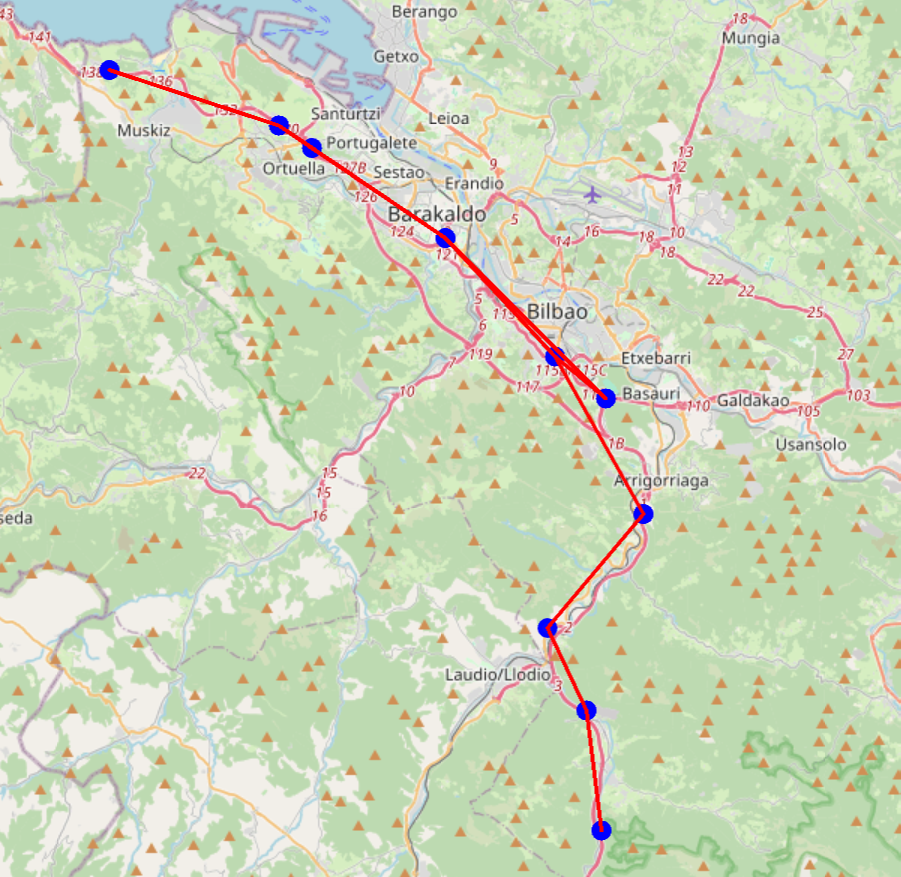
\includegraphics[width=0.5\linewidth]{includes/cap5/source_id_1_meters_mask.png}
	\caption{Distribución espacial de sensores para Gobierno Vasco (sourceId 1).}
	\label{fig:sensores_sid1}
\end{figure}

\begin{figure}[H]
	\centering
	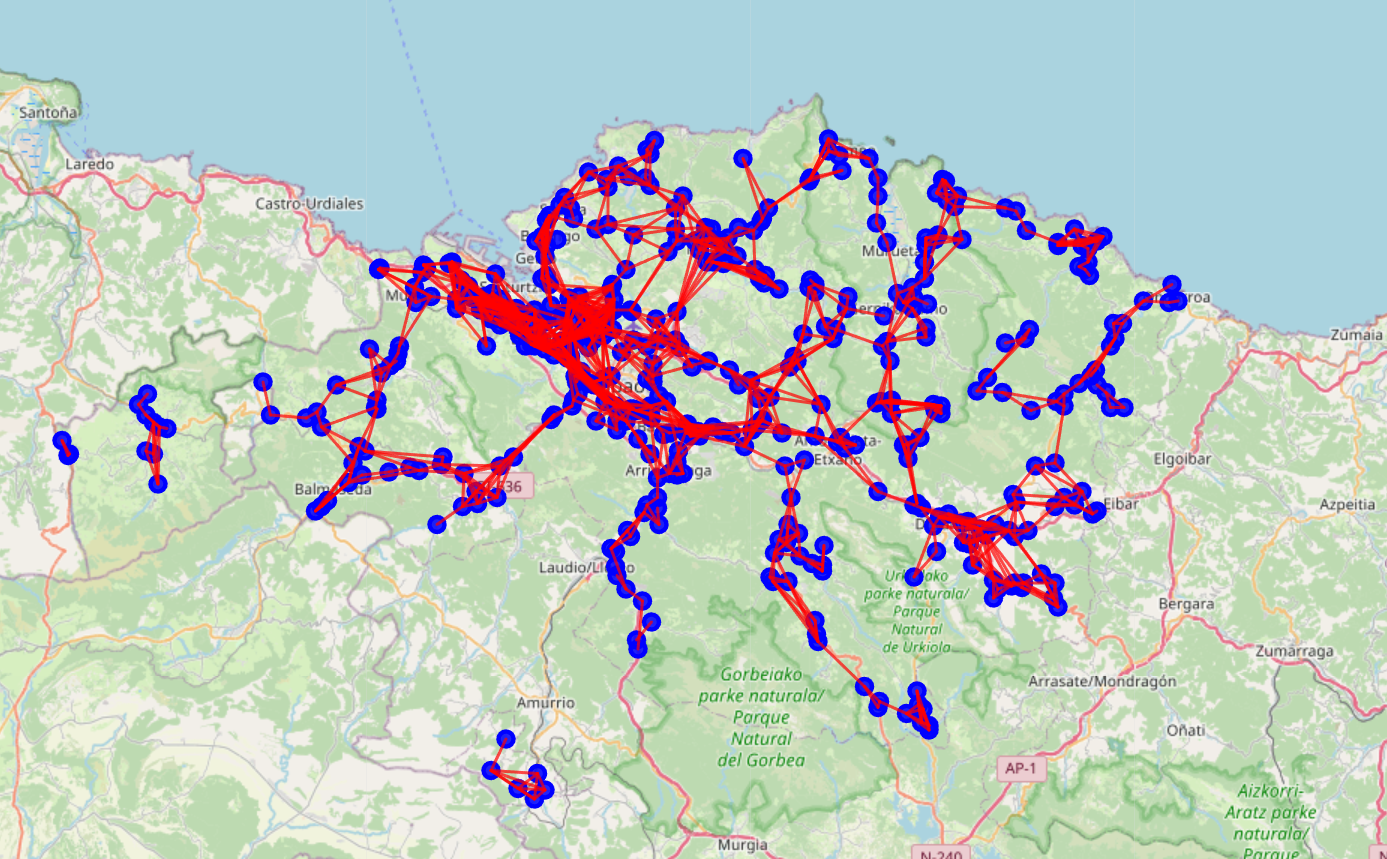
\includegraphics[width=0.7\linewidth]{includes/cap5/source_id_2_meters_mask.png}
	\caption{Distribución espacial de sensores para Diputación Foral de Bizkaia (sourceId 2).}
	\label{fig:sensores_sid2}
\end{figure}

\begin{figure}[H]
	\centering
	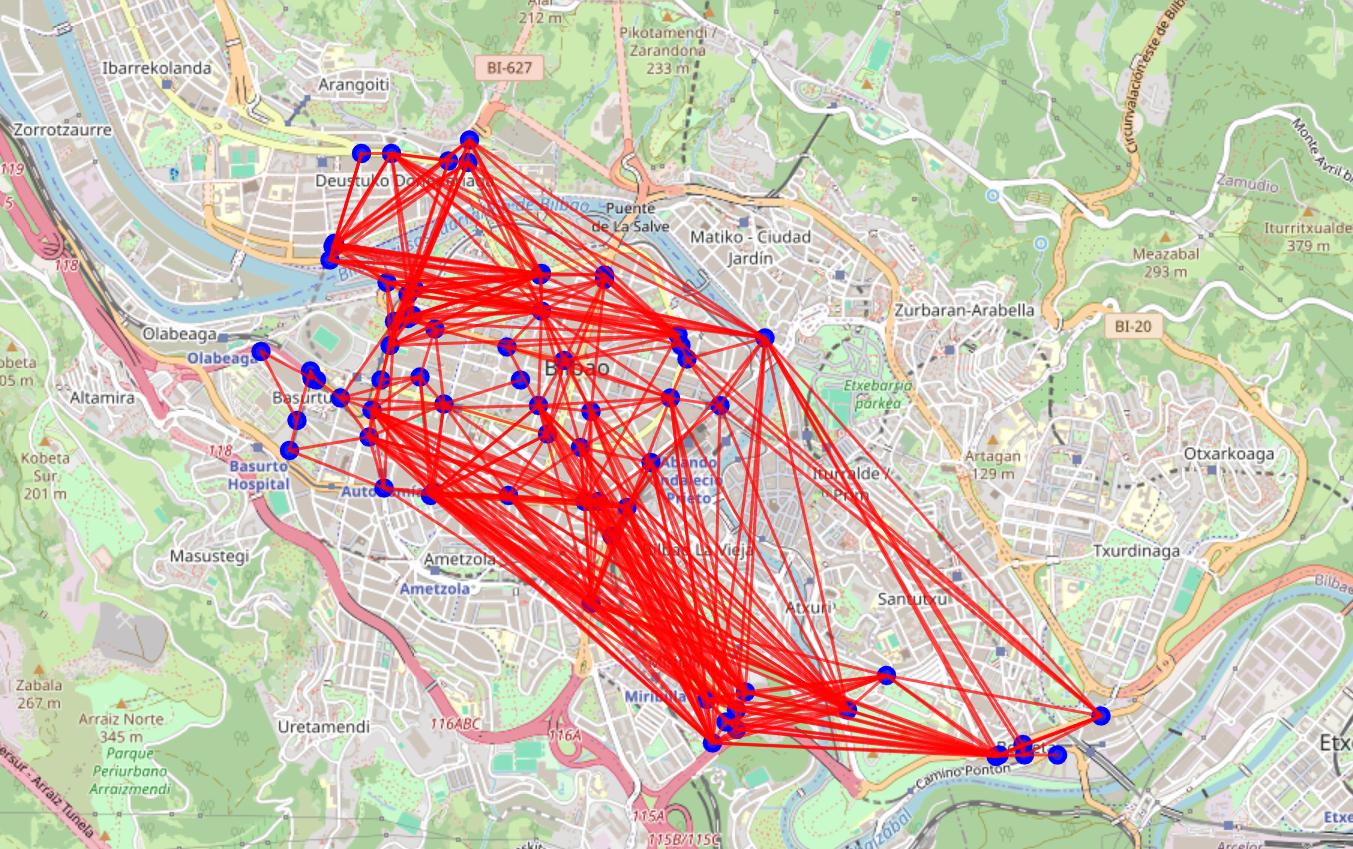
\includegraphics[width=0.7\linewidth]{includes/cap5/source_id_5_meters_mask.png}
	\caption{Distribución espacial de sensores para Ayuntamiento de Bilbao (sourceId 5).}
	\label{fig:sensores_sid5}
\end{figure}

A partir del grafo de sensores se puede derivar la matriz de adyacencia, que resulta clave para la aplicación de técnicas de enmascaramiento espacial y la explotación de correlaciones topológicas en los modelos de predicción.

\subsubsection*{Máscaras espaciales (solo para Trafficformer)}

Las máscaras espaciales permiten restringir el campo de atención del modelo, indicando qué sensores deben influenciarse entre sí durante el proceso de autoatención.

Se ha diseñado una arquitectura extensible de generación de máscaras, implementada en el paquete \texttt{mask}, con dos estrategias principales:

\begin{itemize}
	\item \texttt{BinarySpatialMaskStrategy}: enmascaramiento binario según distancia máxima.
	\item \texttt{OSMPathSpatialMaskStrategy}: estrategia principal utilizada, basada en conectividad vial real extraída de OpenStreetMap.
\end{itemize}

Estas máscaras se construyen en formato tensorial y se almacenan para su reutilización durante los entrenamientos posteriores.

\subsubsection*{Serialización y persistencia}

Todos los tensores generados (entradas, salidas, máscaras) se serializan en disco utilizando formatos como \texttt{.npz} y \texttt{.json}. Estos ficheros se almacenan de forma organizada por combinación de modelo y fuente de datos, y se respaldan en MinIO para garantizar su disponibilidad en posteriores ejecuciones.

Esta estrategia de persistencia permite:

\begin{itemize}
	\item Acelerar la experimentación al evitar preprocesado redundante.
	\item Asegurar reproducibilidad al asociar cada dataset a su configuración original.
	\item Compatibilidad con entornos remotos como AWS, donde se montan los datasets desde MinIO.
\end{itemize}

\subsection{Descripción de los modelos}
\label{sec:descripcion_modelos}

\begin{comment}
	- Explicación y justificación del modelo MLP y del modelo Trafficformer, apoyándose en tus propias docstrings y esquemas de arquitectura.
	- Tabla resumen de los principales hiperparámetros y variantes experimentadas.
\end{comment}

Durante el desarrollo de este trabajo se han implementado dos tipos de modelos de aprendizaje profundo para la predicción del flujo vehicular: un modelo base tipo perceptrón multicapa (MLP) y una arquitectura avanzada basada en Transformers denominada \texttt{Trafficformer}. Ambos modelos han sido implementados en PyTorch y diseñados para ajustarse al mismo pipeline de datos, permitiendo una comparación directa en términos de rendimiento y eficiencia.

\subsubsection*{Perceptrón Multicapa (MLP)}

El modelo \texttt{MLP}, implementado en el fichero \texttt{mlp\_enhanced.py}, actúa como modelo base para el conjunto de experimentos. Su arquitectura consiste en una serie de capas completamente conectadas (\texttt{Linear}), separadas por funciones de activación \texttt{ReLU}, normalización por lotes (\texttt{BatchNorm1d}) y capas de regularización \texttt{Dropout}.

Cada entrada al modelo consiste en un vector plano que concatena todas las variables relevantes para un conjunto de sensores a lo largo de una ventana temporal. No se incorpora ninguna estructura espacial, por lo que no hay noción de relaciones entre sensores.

El objetivo de este modelo es servir de referencia base o \textit{baseline}, tanto en términos de complejidad como de rendimiento, permitiendo comparar sus resultados con arquitecturas más sofisticadas.

En la Figura~\ref{fig:mlp_enhanced_vertical} 
 de capas.

\begin{figure}[H]
	\centering
	\begin{tikzpicture}[
		node distance=1.5cm,
		every node/.style={font=\small, align=center},
		box/.style={draw, rounded corners, minimum width=6.2cm, minimum height=1cm, fill=gray!5},
		arrow/.style={-Latex, thick}
		]
		% Nodes
		\node[box] (input) {[Input: batch, num\_meters, seq\_len, num\_features]};
		\node[box, below=of input] (flatten) {Flatten};
		\node[box, below=of flatten] (linear1) {Linear $\rightarrow$ hidden\_dim\\ReLU + BatchNorm + Dropout};
		\node[box, below=of linear1] (linear2) {Linear $\rightarrow$ hidden\_dim\\ReLU + BatchNorm + Dropout};
		\node[box, below=of linear2] (linear3) {Linear $\rightarrow$ 1};
		\node[box, below=of linear3] (reshape) {Reshape $\rightarrow$ batch $\times$ num\_meters};
		\node[box, below=of reshape] (output) {Output};
		
		% Arrows
		\draw[arrow] (input) -- (flatten);
		\draw[arrow] (flatten) -- (linear1);
		\draw[arrow] (linear1) -- (linear2);
		\draw[arrow] (linear2) -- (linear3);
		\draw[arrow] (linear3) -- (reshape);
		\draw[arrow] (reshape) -- (output);
	\end{tikzpicture}
	\caption{Esquema lógico del flujo de capas en el modelo \texttt{MLP}.}
	\label{fig:mlp_enhanced_vertical}
\end{figure}

El comportamiento del modelo está condicionado por varios parámetros configurables en su constructor:

\begin{itemize}
	\item \texttt{seq\_len}: longitud de la ventana temporal. Determina el número de pasos hacia atrás que observa el modelo por sensor. Ejemplo: 8, para las últimas 4 horas.
	\item \texttt{num\_features}: número de variables por paso temporal (meteorológicas, calendario, incidencias, etc.).
	\item \texttt{num\_meters}: cantidad de sensores simultáneos a predecir en una sola muestra.
	\item \texttt{hidden\_dim}: dimensión de las capas ocultas (\textbf{por defecto: 128}).
	\item \texttt{dropout}: probabilidad de desactivación aleatoria de neuronas durante el entrenamiento (\textbf{por defecto: 0.2}).
\end{itemize}

Estos parámetros permiten ajustar la capacidad del modelo a distintos tamaños de entrada y configuraciones experimentales, manteniendo una estructura modular y flexible.

\subsubsection*{Trafficformer}

El modelo \texttt{Trafficformer}, implementado en el fichero \texttt{trafficformer.py} e incluido en el \hyperref[anexo:codigo_trafficformer]{Anexo~E}, representa una evolución arquitectónica de los Transformers tradicionales adaptada al contexto específico de predicción de tráfico multivariable. A diferencia de las redes densas como el MLP, esta arquitectura se construye con el propósito de capturar de forma simultánea dependencias temporales a lo largo de una ventana de observación y relaciones espaciales entre sensores distribuidos por la red viaria.

Cada entrada al modelo es un tensor de cuatro dimensiones con forma \texttt{[batch, num\_nodes, seq\_len, num\_features]}, donde cada nodo (o sensor) contiene una secuencia temporal de medidas multivariantes. A este tensor se le aplica una codificación posicional sinusoidal, que permite al modelo distinguir la posición relativa de cada instante de tiempo dentro de la secuencia, ya que carece de una estructura recurrente que imponga orden implícito.

Seguidamente, cada nodo procesa localmente su secuencia temporal a través de un extractor de características basado en un perceptrón multicapa (\texttt{MLP}), dotado de capas \texttt{Linear}, activaciones \texttt{ReLU}, normalización \texttt{LayerNorm} y \texttt{Dropout}. Esto da lugar a un embedding por nodo que encapsula su evolución temporal reciente.

Una vez obtenidos estos embeddings, se procede a su procesamiento mediante un bloque encoder compuesto por múltiples capas Transformer apiladas. Estas capas aplican mecanismos de atención multi-cabezal (\texttt{MultiheadAttention}) modificados con una máscara espacial. Esta máscara restringe selectivamente la atención entre pares de sensores en función de su proximidad geográfica o conectividad vial, impidiendo que el modelo derive patrones entre sensores inconexos o lejanos. Esta técnica es especialmente útil en entornos urbanos donde la correlación entre sensores es local y estructural. El uso de máscaras basadas en grafos viales —derivados, por ejemplo, de OpenStreetMap— permite guiar la atención del modelo hacia relaciones físicamente plausibles.

Esta operación se ilustra esquemáticamente en la Figura~\ref{fig:attention_masking}, donde puede observarse cómo, para un nodo dado (por ejemplo, A), el mecanismo de atención restringe las relaciones posibles únicamente a aquellos nodos (como B o D) con los que mantiene una conexión válida según la máscara espacial predefinida. Los nodos no conectados —como C— quedan excluidos del proceso de atención mediante un enmascaramiento explícito. Este mecanismo refuerza la inductiva de la arquitectura, dotándola de una priorización estructural sobre la red vial que mejora la generalización y reduce la posibilidad de sobreajuste a correlaciones espurias.

\begin{figure}[H]
	\centering
	\begin{tikzpicture}[
		node distance=1.8cm,
		every node/.style={font=\small, align=center},
		box/.style={draw, rounded corners, minimum width=5.5cm, minimum height=1cm, fill=gray!5},
		arrow/.style={-Latex, thick}
		]
		% Nodes
		\node[box] (A) {Nodo A (sensor 1)};
		\node[box, below=of A] (att) {Atención multi-cabezal\\Q (query) $\leftarrow$ Nodo A\\K, V (keys, values) $\leftarrow$ Nodos B, C, D, E, ...};
		\node[box, below=of att] (mask) {Máscara espacial (M)\\[2pt]
			M[A][B] = 1 $\rightarrow$ se permite la atención\\
			M[A][C] = 0 $\rightarrow$ atención bloqueada\\
			M[A][D] = 1 $\rightarrow$ se permite la atención\\
			\textellipsis};
		\node[box, below=of mask] (rest) {Atención restringida por máscara};
		\node[box, below=of rest] (embed) {Embedding enriquecido del nodo A};
		
		% Arrows
		\draw[arrow] (A) -- (att);
		\draw[arrow] (att) -- (mask);
		\draw[arrow] (mask) -- (rest);
		\draw[arrow] (rest) -- (embed);
	\end{tikzpicture}
	\caption{Aplicación de la máscara espacial en el mecanismo de atención de \texttt{Trafficformer}.}
	\label{fig:attention_masking}
\end{figure}

Tras el bloque de atención se encuentra una red \texttt{FeedForward} con normalización y conexiones residuales, que complementa la capacidad de aprendizaje no lineal de la arquitectura. Finalmente, se aplica un bloque predictor por nodo, implementado como un MLP con estructura \texttt{Linear → LayerNorm → ReLU → Linear}, que emite la predicción del volumen de tráfico esperado en el próximo instante temporal.

El flujo completo de capas puede representarse de forma esquemática como sigue:

\begin{figure}[H]
	\centering
	\begin{tikzpicture}[
		node distance=1.8cm,
		every node/.style={font=\small, align=center},
		box/.style={draw, rounded corners, minimum width=6.2cm, minimum height=1cm, fill=gray!5},
		arrow/.style={-Latex, thick}
		]
		% Nodes
		\node[box] (input) {[Input: batch, num\_nodes, seq\_len, num\_features]};
		\node[box, below=of input] (posenc) {Positional Encoding};
		\node[box, below=of posenc] (mlp) {Temporal Feature Extractor\\MLP + LayerNorm + Dropout};
		\node[box, below=of mlp] (encoder) {Encoder Layer $\times$ N:\\Spatial Multi-Head Attention\\+ FeedForward + Residual};
		\node[box, below=of encoder] (pred) {Predictor MLP:\\Linear $\rightarrow$ LayerNorm $\rightarrow$ ReLU $\rightarrow$ Linear};
		\node[box, below=of pred] (output) {[Output: batch $\times$ num\_nodes]};
		
		% Arrows
		\draw[arrow] (input) -- (posenc);
		\draw[arrow] (posenc) -- (mlp);
		\draw[arrow] (mlp) -- (encoder);
		\draw[arrow] (encoder) -- (pred);
		\draw[arrow] (pred) -- (output);
	\end{tikzpicture}
	\caption{Esquema lógico del flujo de capas del modelo \texttt{Trafficformer}.}
	\label{fig:trafficformer_vertical}
\end{figure}

Cabe destacar que el modelo ha sido diseñado para ser altamente configurable, permitiendo ajustar su capacidad expresiva a distintos conjuntos de datos y requisitos computacionales. Entre los principales hiperparámetros se encuentran:

\begin{itemize}
	\item \texttt{seq\_len}: número de pasos temporales observados por nodo.
	\item \texttt{num\_features}: cantidad de variables por instante temporal.
	\item \texttt{embedding\_dim}: dimensión del vector que representa cada nodo tras el extractor de características.
	\item \texttt{num\_heads}: número de cabezales en el mecanismo de atención.
	\item \texttt{num\_layers}: número de capas encoder apiladas.
	\item \texttt{ff\_hidden\_dim}: tamaño intermedio en la red feedforward de cada encoder.
	\item \texttt{dropout}: tasa de desactivación de unidades durante el entrenamiento.
\end{itemize}

Esta flexibilidad, unida a su capacidad para integrar estructura espacial, convierte a \texttt{Trafficformer} en una solución avanzada para la predicción de tráfico en entornos reales complejos, como el caso de estudio abordado en este trabajo.

\subsection{Diseño experimental y combinaciones}
\label{sec:diseño_exp_combinaciones}

Para evaluar de forma rigurosa el rendimiento de las distintas arquitecturas propuestas, se ha diseñado un conjunto exhaustivo de experimentos que cubre diversas combinaciones de modelos, hiperparámetros y fuentes de datos. En concreto, el total de combinaciones generadas asciende a \textbf{120 experimentos}, resultado de combinar las 3 fuentes de datos preparadas (Gobierno Vasco, Diputación Foral de Bizkaia y Ayuntamiento de Bilbao), 2 arquitecturas principales (MLP y Trafficformer), y 20 configuraciones distintas de hiperparámetros. Cada uno de estos experimentos ha sido ejecutado de forma independiente y almacenado como notebook reproducible.

El diseño factorial considera dos modelos principales: \texttt{MLP} como base lineal y \texttt{Trafficformer} como modelo avanzado con atención espacial. A su vez, se han evaluado estas arquitecturas sobre tres conjuntos de datos procedentes de distintas fuentes institucionales, representadas por los identificadores \texttt{source\_id = 1, 2, 5}.

Cada modelo ha sido entrenado utilizando un conjunto diverso de combinaciones de hiperparámetros. En la Tabla~\ref{tab:experimentos_resumen} se presentan los valores explorados para cada parámetro, clasificados por arquitectura.

\begin{table}[H]
	\centering
	\small
	\caption{Configuraciones experimentales evaluadas}
	\label{tab:experimentos_resumen}
	\begin{tabularx}{\textwidth}{
			>{\centering\arraybackslash}c
			>{\centering\arraybackslash}c
			>{\centering\arraybackslash}c
			>{\centering\arraybackslash}c
			>{\centering\arraybackslash}c
			>{\centering\arraybackslash}c
			>{\centering\arraybackslash}c
			>{\centering\arraybackslash}c
			>{\centering\arraybackslash}X
	}
		\toprule
		\textbf{SID} & \textbf{M} & \textbf{SL} & \textbf{LR} & \textbf{BS} & \textbf{E/ESP} & \textbf{NH} & \textbf{ED} & \textbf{NL/FF} \\
		\midrule
		1 & MLP           & 4, 8 & 1e-3 / 5e-4 & 64 / 128 & 100 / 10  & -      & -        & - \\
		1 & Trafficformer & 4, 8 & 1e-3 / 5e-4 & 32 / 64  & 120 / 10  & 4 / 8  & 64 / 128 & 4/256 y 6/512 \\
		2 & MLP           & 4, 8 & 1e-3 / 1e-4 & 64 / 128 & 100 / 10  & -      & -        & - \\
		2 & Trafficformer & 4, 8 & 1e-3 / 1e-4 & 32 / 64  & 120 / 10  & 4 / 8  & 64 / 128 & 4/256 y 6/512 \\
		5 & MLP           & 4, 8 & 1e-3 / 5e-4 & 64 / 128 & 100 / 10  & -      & -        & - \\
		5 & Trafficformer & 4, 8 & 1e-3 / 5e-4 & 32 / 64  & 120 / =10 & 4 / 8  & 64 / 128 & 4/256 y 6/512 \\
		\bottomrule
	\end{tabularx}
\end{table}

A continuación, se detallan las combinaciones de hiperparámetros evaluadas en el conjunto de experimentos realizados. Cada uno de estos parámetros ha sido cuidadosamente seleccionado en base a recomendaciones de la literatura científica y su aplicabilidad práctica en modelos de predicción multivariada de series temporales, como se describe seguidamente:

\begin{itemize}
	\item \textbf{SourceId} (SID): La fuente de datos.
	\item \textbf{Modelo} (M): El modelo.
	\item \textbf{SEQ\_LEN} (SL): Los valores 4 y 8 permiten comparar el efecto de ventanas más cortas vs. más largas sobre la precisión y la capacidad de capturar patrones temporales. Es una práctica habitual en \textit{forecasting} experimentar con varias ventanas para encontrar el equilibrio entre capacidad de predicción y sobreajuste.
	\item \textbf{Learning Rate} (LR): 1e-3 es un valor estándar en \textit{deep learning} y recomendado en el propio artículo de Trafficformer~\cite{trafficformer}, pero se elige 5e-4 para realizar el experimento. En el articulo también se cita el empleo de la estrategia ReduceLROnPlateau \cite{ruder2017overviewgradientdescentoptimization}, estrategia que permite reducir el learning rate hasta un umbral en función de la selección de una métrica. Pese a que dicha estrategia está disponible en Pytorch \cite{pytorchReduceLrOnPLateau} se decidió no emplearla por reducir la complejidad del experimento.
	\item \textbf{Batch Size} (BS): Se experimenta con 64 y 128 para MLP, y con 32 y 64 para Trafficformer. Un \textit{batch size} menor en Trafficformer permite reducir el uso de memoria y mejora la generalización en modelos más profundos.
	\item \textbf{Epochs / Early Stopping, Patience} (E/ESP): Se ha limitado el entrenamiento a 100--120 épocas, con un mecanismo de \textit{early stopping} con paciencia de 10 épocas. Esta configuración evita el sobreentrenamiento sin necesidad de vigilancia manual.
	\item \textbf{NUM\_HEADS} (NH) y \textbf{EMBEDDING\_DIM} (ED): Las combinaciones evaluadas (4/64 y 8/128) reflejan el equilibrio entre capacidad representacional y coste computacional. Un mayor número de cabezas puede capturar relaciones más complejas entre sensores.
	\item \textbf{NUM\_LAYERS} (NL) y \textbf{FF\_HIDDEN\_DIM} (FF): Se han probado configuraciones de 4 capas con 256 dimensiones ocultas y 6 capas con 512. Estos valores están alineados con los recomendados en el artículo original y en benchmarks del estado del arte.
\end{itemize}

Cada experimento fue registrado y monitorizado utilizando la plataforma \texttt{Weights \& Biases}, lo que permitió realizar un análisis sistemático posterior y facilitar la selección de los mejores modelos por fuente de datos y arquitectura. Para facilitar la reproducibilidad y la trazabilidad de los resultados, todos los notebooks están numerados de forma consistente e incluyen visualizaciones, métricas y configuración exacta de entrenamiento.

En el \hyperref[anexo:combinaciones_exp]{Anexo~F} se pueden consultar las diferentes combinaciones experimentales propuestas.

\subsection{Proceso de entrenamiento y selección de mejores modelos}
\label{sec:entrenamiento_mej_modelos}

El proceso de entrenamiento de los modelos se ha realizado bajo un entorno controlado y reproducible, siguiendo las mejores prácticas en experimentación con redes neuronales. Para ello, se han desarrollado cuadernos Jupyter donde se define de manera explícita cada paso del ciclo experimental: carga de datos, configuración del entorno, definición del modelo, entrenamiento, evaluación y registro de resultados.

\subsubsection*{Configuración y reproducibilidad}  
El entorno de trabajo se inicializa con la carga de variables de entorno desde ficheros \texttt{.env}, estableciendo parámetros como la conexión a la base de datos MongoDB, claves de autenticación para \textit{Weights \& Biases} (Wandb), y valores por defecto de hiperparámetros como \texttt{batch size}, \texttt{learning rate}, \texttt{dropout} o \texttt{hidden dimensions}. Se fija una semilla aleatoria global para asegurar la reproducibilidad entre ejecuciones, controlando el estado de generación de números aleatorios tanto de \texttt{NumPy}, \texttt{Python} como de \texttt{PyTorch} (CPU y GPU).

\subsubsection*{Carga del dataset y preparación}  
Se emplea una clase personalizada \texttt{TrafficDataset}, diseñada para conectarse directamente a la base de datos y construir un conjunto de muestras a partir de una ventana temporal configurable (\texttt{SEQ\_LEN}). El conjunto de datos incluye tanto variables numéricas escaladas (\texttt{StandardScaler}), como categóricas codificadas (\texttt{OneHotEncoder}) y booleanas convertidas a \texttt{float} con valores binarios. Las variables faltantes se imputan de forma segura mediante media (\texttt{mean}) para variables continuas y con cero para booleanos. La división de datos se realiza de forma estratificada y reproducible en tres subconjuntos: entrenamiento (70\%), validación (20\%) y test (10\%).

\subsubsection*{Máscara espacial y visualización}  
Para los modelos tipo Transformer, se genera una máscara espacial binaria que codifica qué sensores de tráfico pueden atenderse entre sí, basada en criterios geográficos extraídos desde OpenStreetMap (vía GraphML). Esta máscara se emplea durante el mecanismo de atención multi-cabezal. Se valida la consistencia entre los sensores del dataset y la máscara, y se genera una visualización interactiva de la red de sensores y sus enlaces espaciales, posteriormente registrada como artefacto en Wandb.

\subsubsection*{Inicialización del modelo y optimización}  
El modelo se instancia según el tipo elegido (\texttt{TrafficMLPEnhanced} o \texttt{Trafficformer}), utilizando parámetros definidos al inicio del experimento. El criterio de pérdida utilizado es el error cuadrático medio (\texttt{MSELoss}), y el optimizador elegido es \texttt{AdamW}, con tasa de aprendizaje inicial y \texttt{weight decay} ajustables. El modelo y el criterio son registrados en Wandb, junto con los hiperparámetros y la configuración del experimento.

\subsubsection*{Entrenamiento supervisado y \textit{early stopping}}  
El bucle de entrenamiento se ejecuta durante un máximo de 100--120 épocas, con activación de un mecanismo de \textit{early stopping} basado en la pérdida de validación con una paciencia de 10 épocas. Por cada época, se computan las métricas \texttt{MSE}, \texttt{MAE}, \texttt{RMSE}, \texttt{MAPE} y \texttt{R\textsuperscript{2}} para los tres subconjuntos (train, val, test). Además, se monitoriza el uso de memoria RAM y GPU, el tiempo de inferencia por muestra y la duración total por época.

En cada iteración se guardan:

\begin{itemize}
	\item Un \textit{checkpoint} del estado actual del modelo, optimizador y estados aleatorios.
	\item La historia de métricas en un fichero CSV.
	\item El mejor modelo según pérdida de validación.
\end{itemize}

\subsubsection*{Evaluación y seguimiento}  
Al finalizar el entrenamiento, se guarda el modelo final, se registra el tiempo total del proceso y se finaliza la sesión de WandB. Además, se generan gráficas para cada métrica de evaluación, comparando la evolución entre entrenamiento y validación. La mejor época se corresponde con la mínima pérdida de validación y se resalta en cada gráfica. Estas curvas permiten detectar patrones de sobreentrenamiento, estancamiento o mejoras progresivas en el aprendizaje.

\begin{figure}[H]
	\centering
	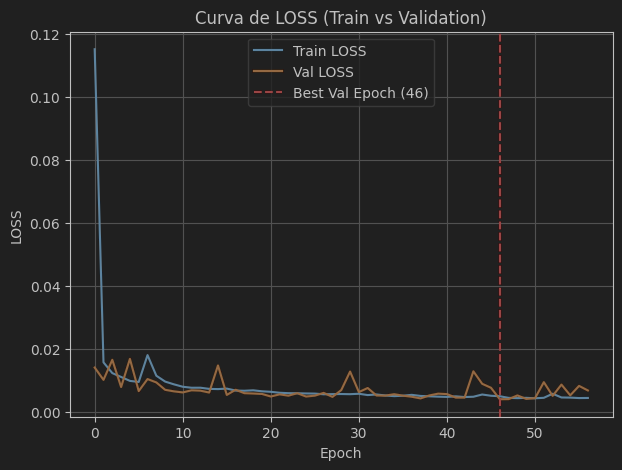
\includegraphics[width=0.5\textwidth]{includes/cap5/loss_curve_example.png}
	\caption{Curvas de evolución de pérdida para entrenamiento y validación, con indicación de la mejor época.}
	\label{fig:loss_curve_example}
\end{figure}

\subsubsection*{Registro de resultados y comparación}  
Cada experimento queda documentado y reproducible mediante artefactos almacenados en el sistema de ficheros y sincronizados con la plataforma \textit{Weights \& Biases}. Esto incluye mapas de sensores, configuración exacta, métricas por época, curvas de entrenamiento y modelos entrenados. El historial completo permite comparar el rendimiento de diferentes combinaciones de hiperparámetros, tanto a nivel visual como mediante agregación tabular.

	\clearpage
	\section{Evaluación, comparación de modelos y resultados}
\label{sec:evaluacion}

%
% Para citar: 
% 	(ver Sección~\ref{sec:dataset_arquitectura})
% 	como se describe en la Sección~\nameref{sec:dataset_arquitectura})
%

\subsection{Resultados experimentales}
\label{sec:resultados_exp}

\begin{comment}
	- Presentación de los resultados finales:
	- Tablas y/o gráficos para las métricas más relevantes (MAE, RMSE, R2, MAPE...) para cada experimento y cada mejor modelo.
	- Comparativa directa entre MLP y Trafficformer para cada source.
	- Visualizaciones clave (si tienes heatmaps, gráficas de error, etc.).
\end{comment}

Para cada una de las tres fuentes de datos disponibles (\texttt{sourceId} = 1, 2 y 5), se ha seleccionado el mejor modelo entrenado para cada una de las dos arquitecturas evaluadas: \texttt{MLP} y \texttt{Trafficformer}. La selección se ha realizado tomando como criterio el valor mínimo de la métrica de pérdida sobre el conjunto de validación (\texttt{val\_loss}) entre todas las combinaciones de hiperparámetros evaluadas durante el proceso experimental.

En el \hyperref[anexo:resultados_exp]{Anexo~G} se puede consultar la tabla completa de todos los experimentos llevados a cabo junto con los resultados de todas las métricas obtenidas.

En la tabla~\ref{tab:mejores_modelos} se muestran los modelos seleccionados junto con sus respectivas métricas sobre el conjunto de test, así como los valores clave de los hiperparámetros empleados.

\begin{table}[H]
	\centering
	\small
	\caption{Resultados de los mejores modelos por combinación \texttt{sourceId}--arquitectura}
	\label{tab:mejores_modelos}
	\begin{tabularx}{\textwidth}{c | c | c | c | c | c | c | c }
		\toprule
		\textbf{SID} & \textbf{M} & \textbf{EP} & \textbf{VTL} & \textbf{VTMAE} & \textbf{VTRMSE} & \textbf{VTMAPE} & \textbf{VTR2} \\
		\midrule
		1 & mlp           & 67 & 0.000 & 25.327/25.466 & 50.904/38.489 & 1.826/1.853 & 0.743/0.759 \\
		1 & trafficformer & 30 & 0.143 & 19.300/19.125 & 44.298/30.784 & 1.718/1.745 & 0.797/0.822 \\
		2 & mlp           & 30 & 0.000 & 30.967/31.017 & 38.144/38.177 & 1.75e14/1.82e14 & 0.868/0.866 \\
		2 & trafficformer & 96 & 0.002 & 5.787/5.832 & 15.356/15.046 & 1.31e3/1.51e3 & 0.983/0.982 \\
		5 & mlp           & 39 & 0.000 & 216.265/213.850 & 345.766/343.603 & 4.85e5/4.83e5 & 0.523/-1.797 \\
		5 & trafficformer & 29 & 0.153 & 176.356/175.975 & 308.041/306.134 & 1.74e5/1.74e5 & 0.703/0.640 \\
		\bottomrule
	\end{tabularx}
	\vspace{0.5em}
	\begin{minipage}{0.98\textwidth}
	\footnotesize
	\textbf{Leyenda de columnas:} \\
	\textbf{SID}: sourceId. \\
	\textbf{M}: Modelo. \\
	\textbf{EP}: Epoch óptima. \\
	\textbf{VTL}: Validation \& Test Loss. \\
	\textbf{VTMAE}: Validation \& Test MAE. \\
	\textbf{VTRMSE}: Validation \& Test RMSE. \\
	\textbf{VTMAPE}: Validation \& Test MAPE. \\
	\textbf{VTR2}: Validation \& Test $R^2$. \\
	Los valores muy grandes se muestran en notación científica (\texttt{a.eb} significa $a \times 10^{b}$). Decimales reducidos para mejorar la presentación.
	\end{minipage}
\end{table}

%%

A continuación se muestran, para cada una de las combinaciones óptimas de fuente de datos (\texttt{sourceId}) y arquitectura (\texttt{MLP} y \texttt{Trafficformer}), las curvas de evolución de las principales métricas durante el entrenamiento. Estas gráficas permiten visualizar el comportamiento del proceso de aprendizaje en términos de error (loss), precisión (MAE, MAPE, MSE, RMSE), y capacidad explicativa ($R^2$), tanto en entrenamiento como en validación. De este modo, se facilita la identificación de fenómenos de sobreajuste, convergencia y diferencias entre arquitecturas y datasets.

Cada figura agrupa, en formato compacto, las seis métricas principales para cada modelo, mostrando la evolución época a época.

\begin{figure}[H]
	\centering
	\begin{minipage}{0.48\textwidth}
		\centering
		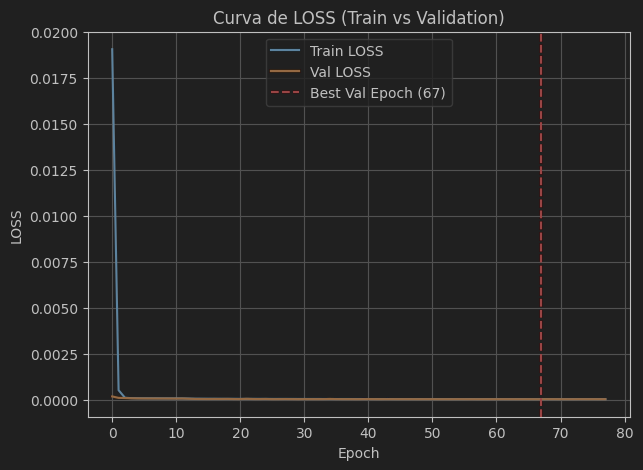
\includegraphics[width=\linewidth]{includes/cap5/graphs/sid1_mlp_loss.png}
		\subcaption{Loss}
		\vspace{0.2cm}
		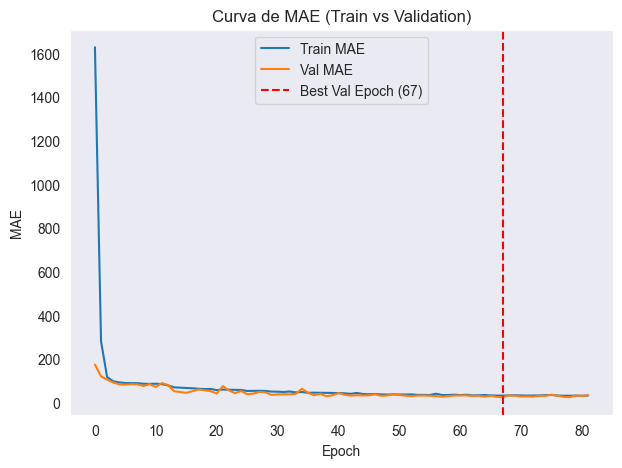
\includegraphics[width=\linewidth]{includes/cap5/graphs/sid1_mlp_mae.png}
		\subcaption{MAE}
		\vspace{0.2cm}
		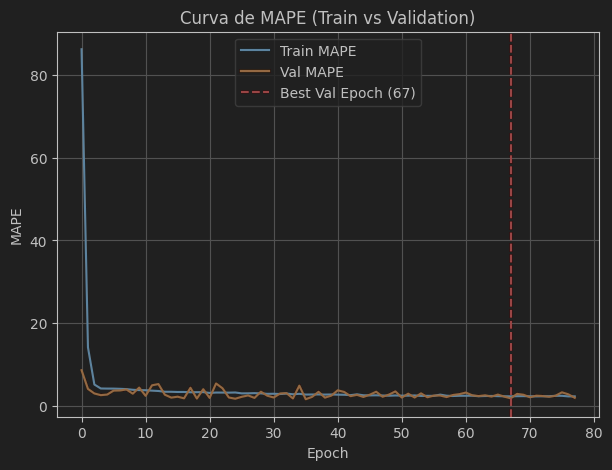
\includegraphics[width=\linewidth]{includes/cap5/graphs/sid1_mlp_mape.png}
		\subcaption{MAPE}
	\end{minipage}
	\hfill
	\begin{minipage}{0.48\textwidth}
		\centering
		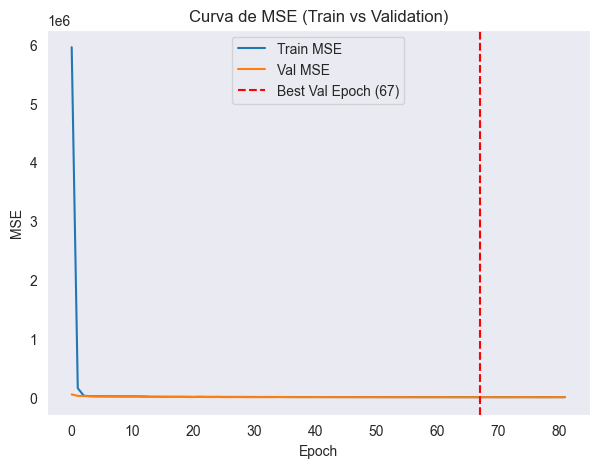
\includegraphics[width=\linewidth]{includes/cap5/graphs/sid1_mlp_mse.png}
		\subcaption{MSE}
		\vspace{0.2cm}
		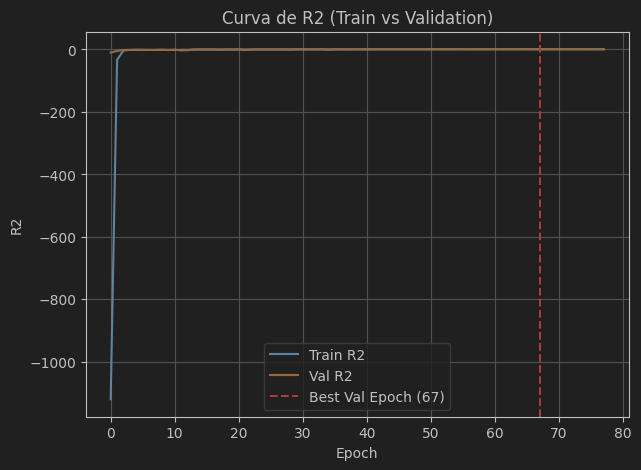
\includegraphics[width=\linewidth]{includes/cap5/graphs/sid1_mlp_r2.png}
		\subcaption{$R^2$}
		\vspace{0.2cm}
		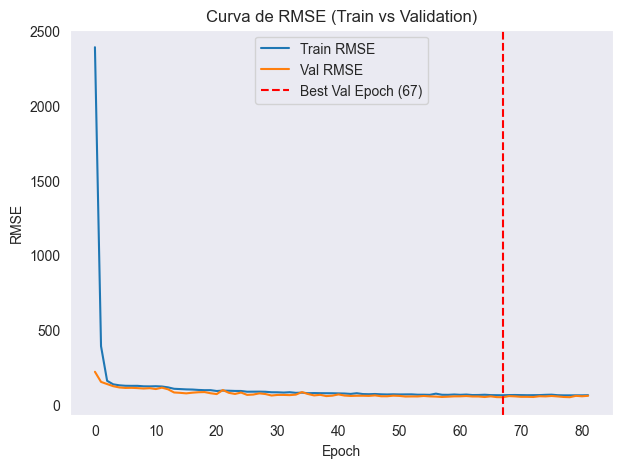
\includegraphics[width=\linewidth]{includes/cap5/graphs/sid1_mlp_rmse.png}
		\subcaption{RMSE}
	\end{minipage}
	\caption{Curvas de entrenamiento para el modelo \texttt{MLP} con sourceId 1.}
	\label{fig:curvas_sid1_mlp}
\end{figure}

\begin{figure}[H]
	\centering
	\begin{minipage}{0.48\textwidth}
		\centering
		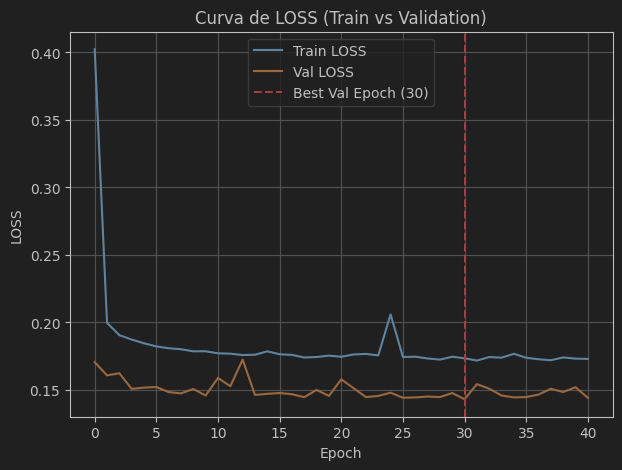
\includegraphics[width=\linewidth]{includes/cap5/graphs/sid1_trafficformer_loss.png}
		\subcaption{Loss}
		\vspace{0.2cm}
		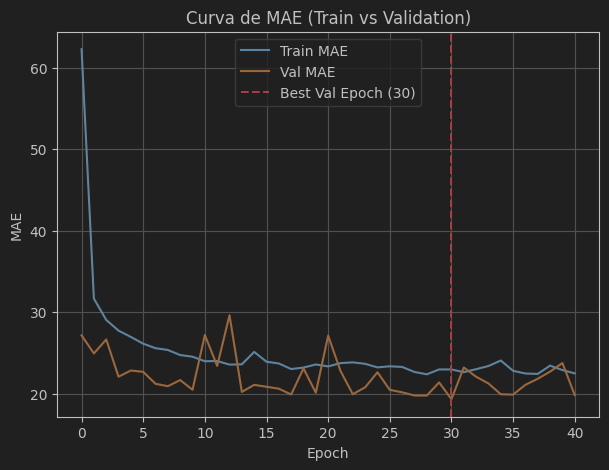
\includegraphics[width=\linewidth]{includes/cap5/graphs/sid1_trafficformer_mae.png}
		\subcaption{MAE}
		\vspace{0.2cm}
		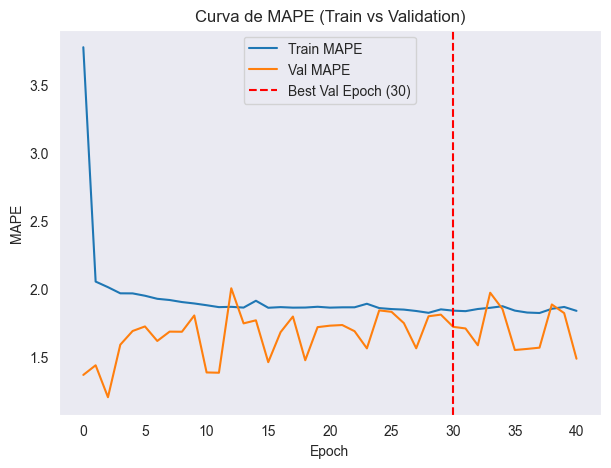
\includegraphics[width=\linewidth]{includes/cap5/graphs/sid1_trafficformer_mape.png}
		\subcaption{MAPE}
	\end{minipage}
	\hfill
	\begin{minipage}{0.48\textwidth}
		\centering
		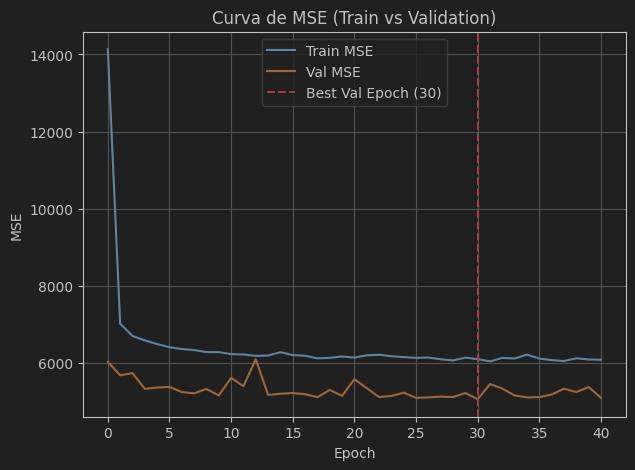
\includegraphics[width=\linewidth]{includes/cap5/graphs/sid1_trafficformer_mse.png}
		\subcaption{MSE}
		\vspace{0.2cm}
		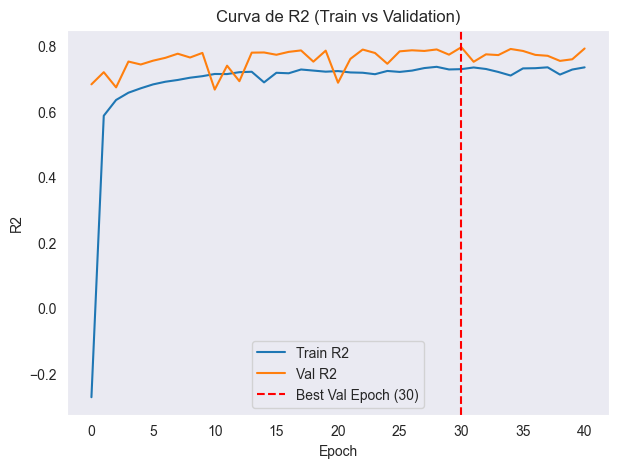
\includegraphics[width=\linewidth]{includes/cap5/graphs/sid1_trafficformer_r2.png}
		\subcaption{$R^2$}
		\vspace{0.2cm}
		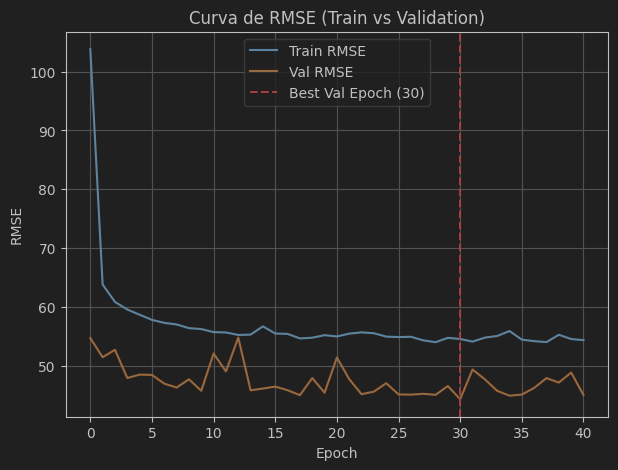
\includegraphics[width=\linewidth]{includes/cap5/graphs/sid1_trafficformer_rmse.png}
		\subcaption{RMSE}
	\end{minipage}
	\caption{Curvas de entrenamiento para el modelo \texttt{Trafficformer} con sourceId 1.}
	\label{fig:curvas_sid1_trafficformer}
\end{figure}

%%

\begin{figure}[H]
	\centering
	\begin{minipage}{0.48\textwidth}
		\centering
		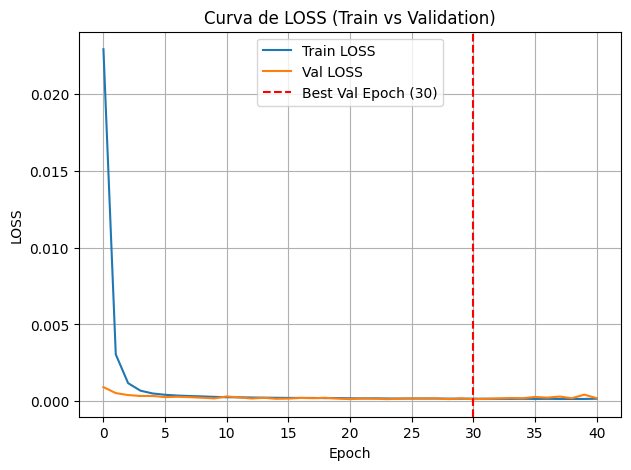
\includegraphics[width=\linewidth]{includes/cap5/graphs/sid2_mlp_loss.png}
		\subcaption{Loss}
		\vspace{0.2cm}
		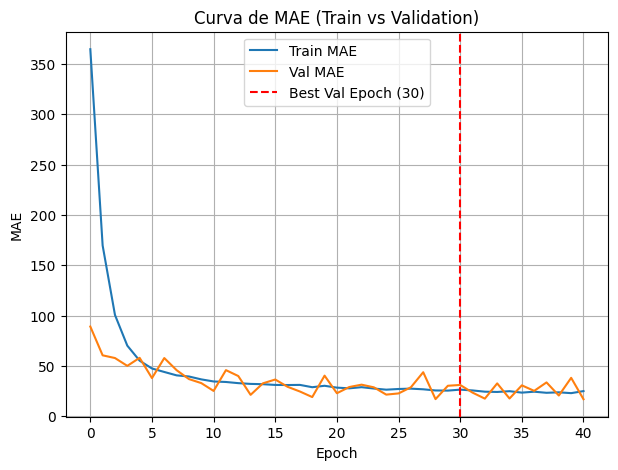
\includegraphics[width=\linewidth]{includes/cap5/graphs/sid2_mlp_mae.png}
		\subcaption{MAE}
		\vspace{0.2cm}
		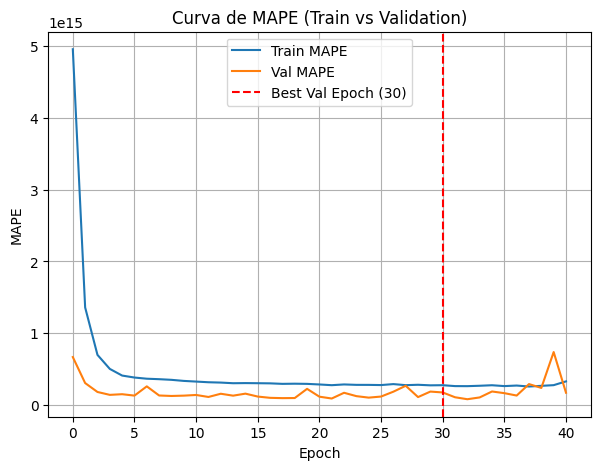
\includegraphics[width=\linewidth]{includes/cap5/graphs/sid2_mlp_mape.png}
		\subcaption{MAPE}
	\end{minipage}
	\hfill
	\begin{minipage}{0.48\textwidth}
		\centering
		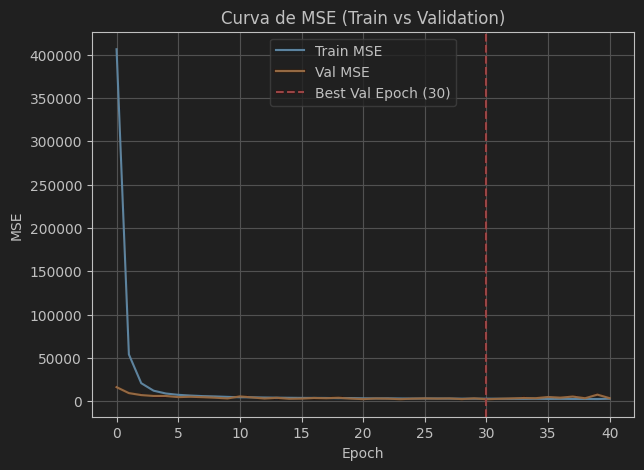
\includegraphics[width=\linewidth]{includes/cap5/graphs/sid2_mlp_mse.png}
		\subcaption{MSE}
		\vspace{0.2cm}
		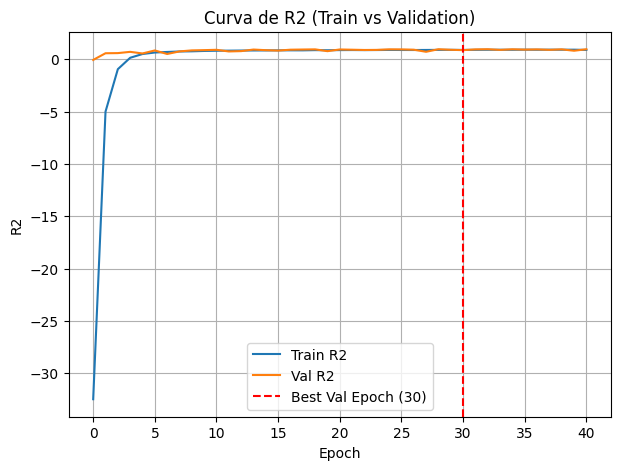
\includegraphics[width=\linewidth]{includes/cap5/graphs/sid2_mlp_r2.png}
		\subcaption{$R^2$}
		\vspace{0.2cm}
		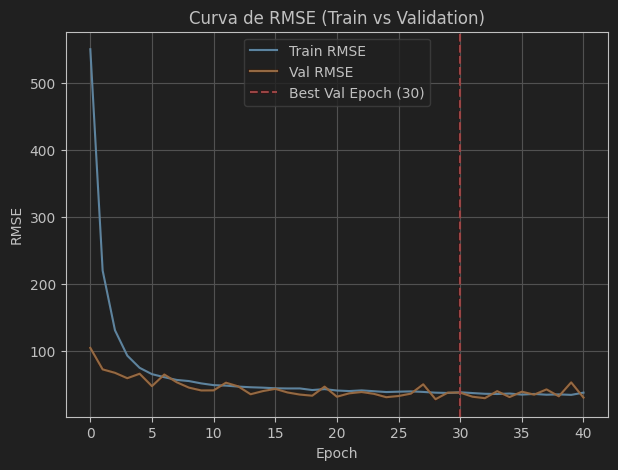
\includegraphics[width=\linewidth]{includes/cap5/graphs/sid2_mlp_rmse.png}
		\subcaption{RMSE}
	\end{minipage}
	\caption{Curvas de entrenamiento para el modelo \texttt{MLP} con sourceId 2.}
	\label{fig:curvas_sid2_mlp}
\end{figure}

\begin{figure}[H]
	\centering
	\begin{minipage}{0.48\textwidth}
		\centering
		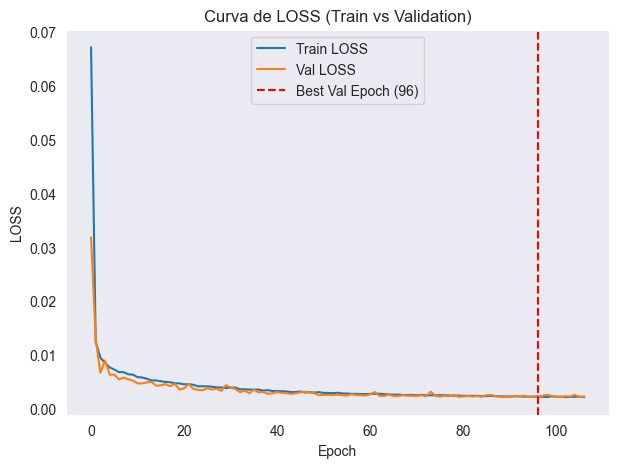
\includegraphics[width=\linewidth]{includes/cap5/graphs/sid2_trafficformer_loss.png}
		\subcaption{Loss}
		\vspace{0.2cm}
		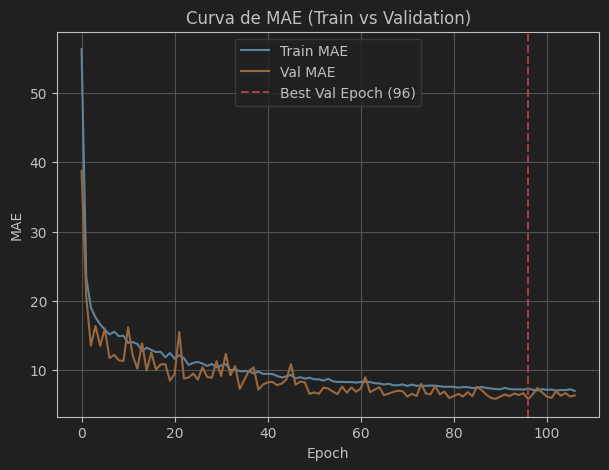
\includegraphics[width=\linewidth]{includes/cap5/graphs/sid2_trafficformer_mae.png}
		\subcaption{MAE}
		\vspace{0.2cm}
		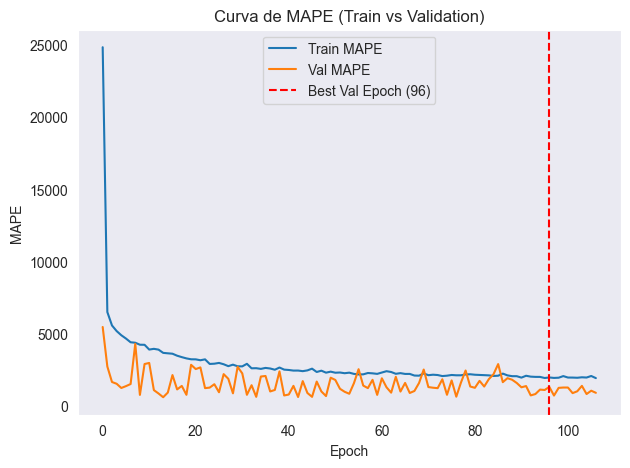
\includegraphics[width=\linewidth]{includes/cap5/graphs/sid2_trafficformer_mape.png}
		\subcaption{MAPE}
	\end{minipage}
	\hfill
	\begin{minipage}{0.48\textwidth}
		\centering
		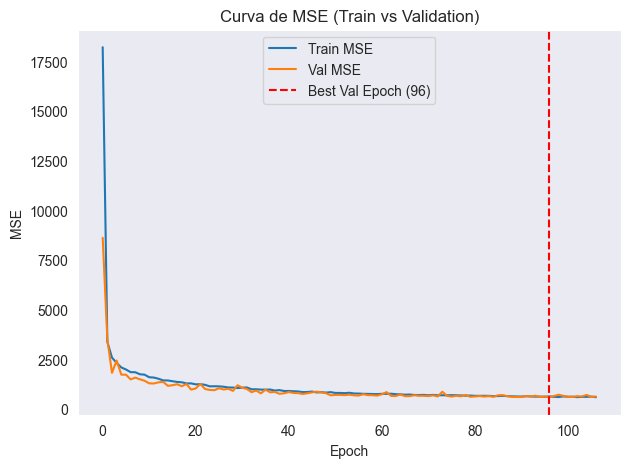
\includegraphics[width=\linewidth]{includes/cap5/graphs/sid2_trafficformer_mse.png}
		\subcaption{MSE}
		\vspace{0.2cm}
		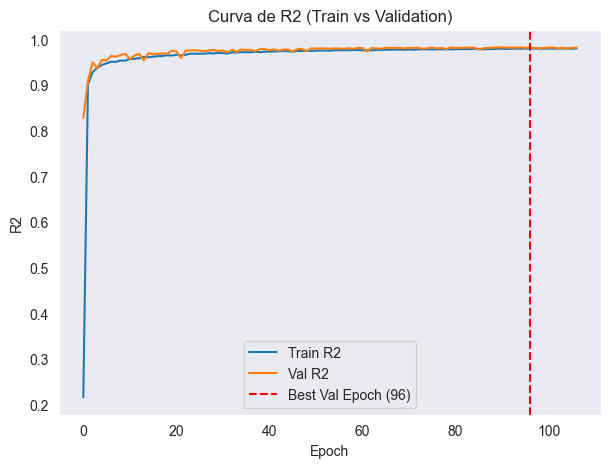
\includegraphics[width=\linewidth]{includes/cap5/graphs/sid2_trafficformer_r2.png}
		\subcaption{$R^2$}
		\vspace{0.2cm}
		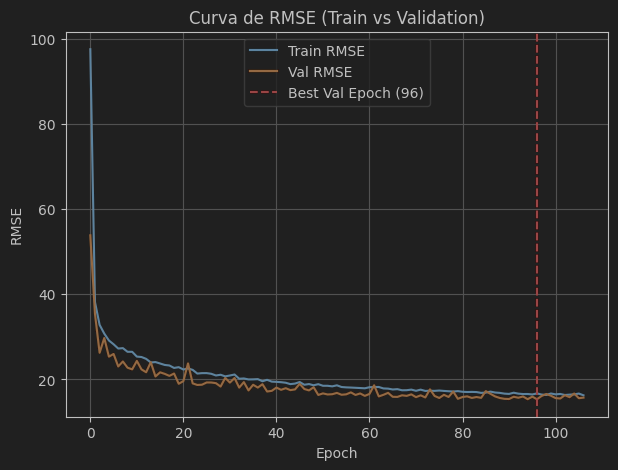
\includegraphics[width=\linewidth]{includes/cap5/graphs/sid2_trafficformer_rmse.png}
		\subcaption{RMSE}
	\end{minipage}
	\caption{Curvas de entrenamiento para el modelo \texttt{Trafficformer} con sourceId 2.}
	\label{fig:curvas_sid2_trafficformer}
\end{figure}

%%

\begin{figure}[H]
	\centering
	\begin{minipage}{0.48\textwidth}
		\centering
		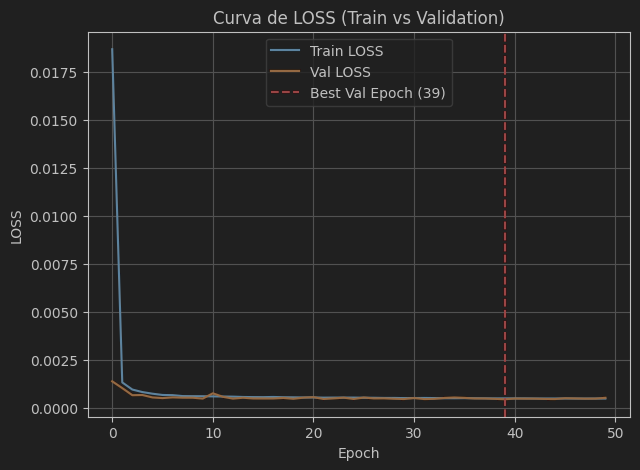
\includegraphics[width=\linewidth]{includes/cap5/graphs/sid5_mlp_loss.png}
		\subcaption{Loss}
		\vspace{0.2cm}
		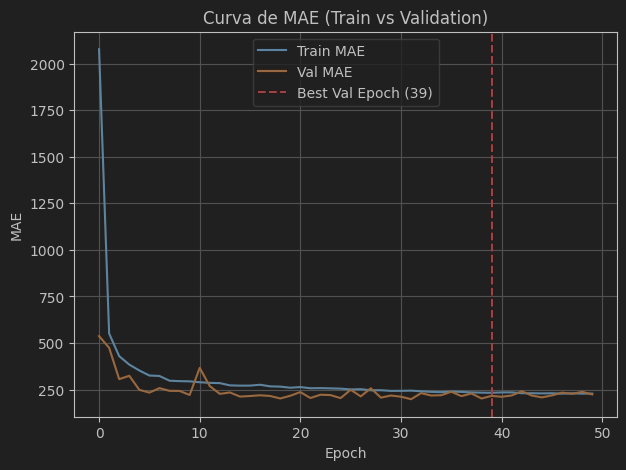
\includegraphics[width=\linewidth]{includes/cap5/graphs/sid5_mlp_mae.png}
		\subcaption{MAE}
		\vspace{0.2cm}
		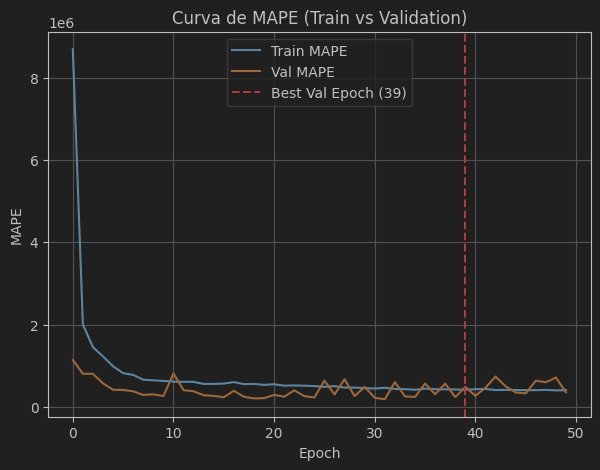
\includegraphics[width=\linewidth]{includes/cap5/graphs/sid5_mlp_mape.png}
		\subcaption{MAPE}
	\end{minipage}
	\hfill
	\begin{minipage}{0.48\textwidth}
		\centering
		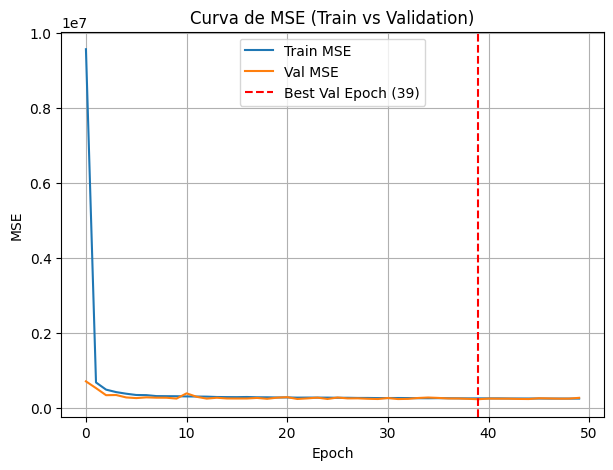
\includegraphics[width=\linewidth]{includes/cap5/graphs/sid5_mlp_mse.png}
		\subcaption{MSE}
		\vspace{0.2cm}
		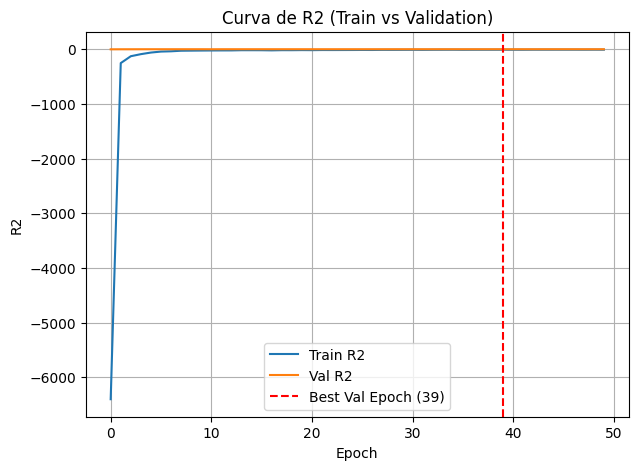
\includegraphics[width=\linewidth]{includes/cap5/graphs/sid5_mlp_r2.png}
		\subcaption{$R^2$}
		\vspace{0.2cm}
		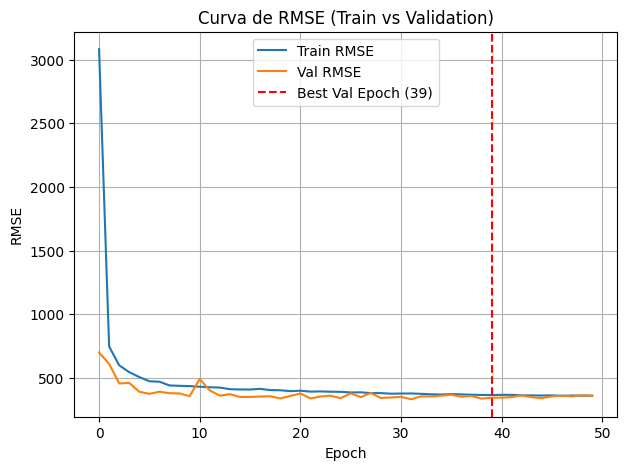
\includegraphics[width=\linewidth]{includes/cap5/graphs/sid5_mlp_rmse.png}
		\subcaption{RMSE}
	\end{minipage}
	\caption{Curvas de entrenamiento para el modelo \texttt{MLP} con sourceId 5.}
	\label{fig:curvas_sid5_mlp}
\end{figure}

\begin{figure}[H]
	\centering
	\begin{minipage}{0.48\textwidth}
		\centering
		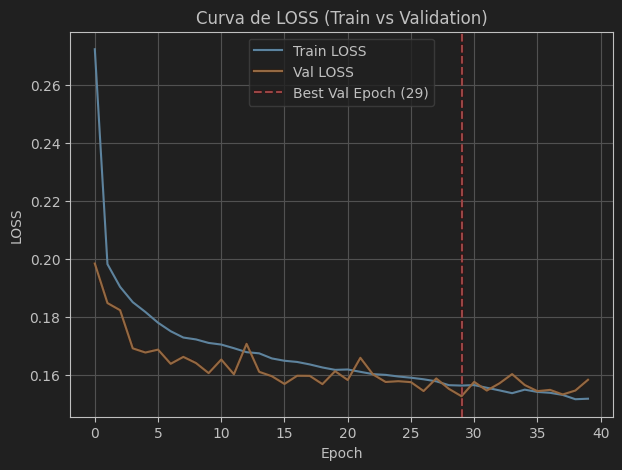
\includegraphics[width=\linewidth]{includes/cap5/graphs/sid5_trafficformer_loss.png}
		\subcaption{Loss}
		\vspace{0.2cm}
		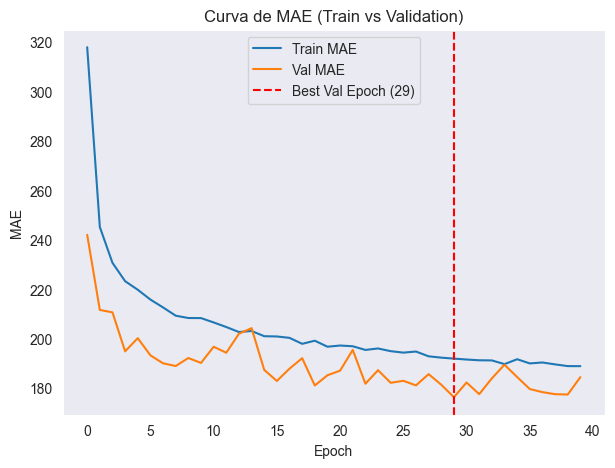
\includegraphics[width=\linewidth]{includes/cap5/graphs/sid5_trafficformer_mae.png}
		\subcaption{MAE}
		\vspace{0.2cm}
		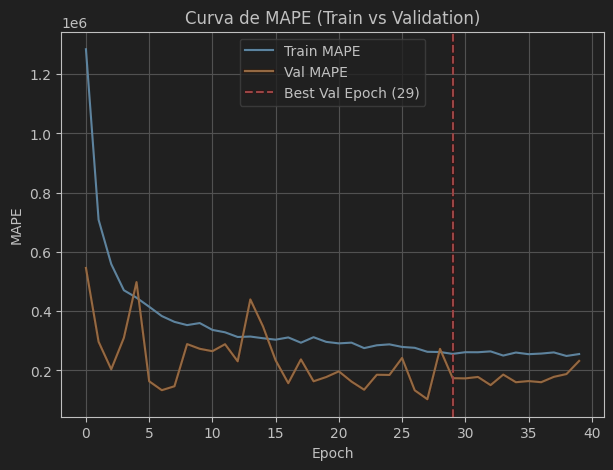
\includegraphics[width=\linewidth]{includes/cap5/graphs/sid5_trafficformer_mape.png}
		\subcaption{MAPE}
	\end{minipage}
	\hfill
	\begin{minipage}{0.48\textwidth}
		\centering
		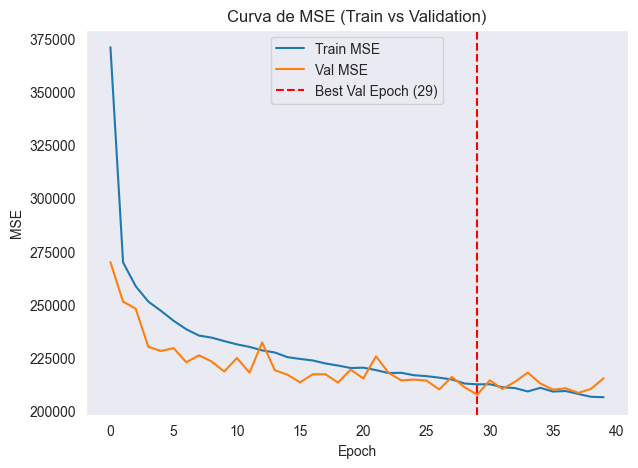
\includegraphics[width=\linewidth]{includes/cap5/graphs/sid5_trafficformer_mse.png}
		\subcaption{MSE}
		\vspace{0.2cm}
		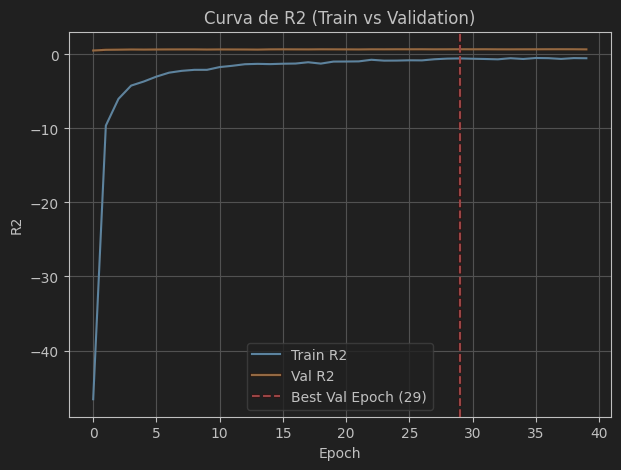
\includegraphics[width=\linewidth]{includes/cap5/graphs/sid5_trafficformer_r2.png}
		\subcaption{$R^2$}
		\vspace{0.2cm}
		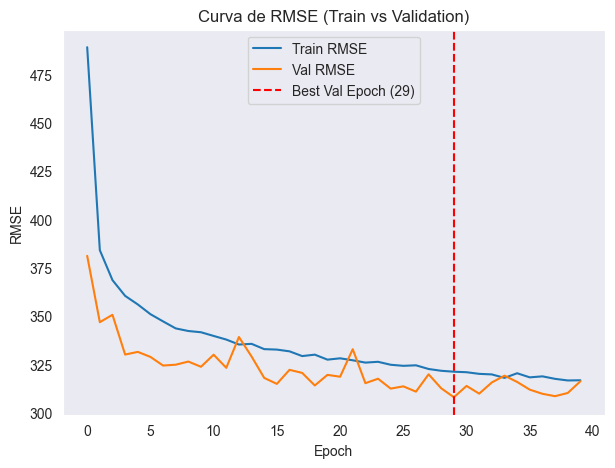
\includegraphics[width=\linewidth]{includes/cap5/graphs/sid5_trafficformer_rmse.png}
		\subcaption{RMSE}
	\end{minipage}
	\caption{Curvas de entrenamiento para el modelo \texttt{Trafficformer} con sourceId 5.}
	\label{fig:curvas_sid5_trafficformer}
\end{figure}

Todas las curvas y métricas detalladas para los 120 experimentos están disponibles en la plataforma \textit{Weights \& Biases}.

%%

\subsection{Discusión y análisis crítico}
\label{sec:discusion_analisis}

\begin{comment}
	- Interpretación de los resultados:
	- ¿Dónde y por qué Trafficformer supera a MLP?
	- ¿Hay algún caso donde no sea así?
	- Relación con lo observado en el estado del arte.
	- Reflexión sobre la influencia de los hiperparámetros, la ventana temporal y el tamaño del batch.
\end{comment}

En esta sección se realiza una evaluación crítica y comparativa de los resultados obtenidos por las dos arquitecturas propuestas (MLP y Trafficformer), para cada una de las tres fuentes de datos analizadas (sourceIds 1, 2 y 5). Se emplean las métricas reportadas en la tabla~\ref{tab:mejores_modelos}, junto con las gráficas de entrenamiento para cada modelo, para ofrecer un análisis detallado sobre la superioridad y limitaciones observadas.

\subsubsection*{Comparativa en sourceId 1}

La comparativa entre modelos MLP (figura~\ref{fig:curvas_sid1_mlp}) y Trafficformer (figura~\ref{fig:curvas_sid1_trafficformer}) muestra claramente la ventaja del modelo Trafficformer. Esta arquitectura obtiene un valor significativamente menor en las métricas de pérdida (loss), MAE, RMSE y MAPE, así como un valor superior en $R^2$. En particular, Trafficformer logra reducir el MAE desde 25.466 hasta 19.125 y el RMSE desde 38.489 hasta 30.784, mostrando una mejor capacidad para capturar las complejidades espaciales y temporales de los datos de tráfico.

El análisis visual de las curvas de entrenamiento evidencia una convergencia más rápida y estable del modelo Trafficformer, alcanzando el punto óptimo en la época 30, notablemente antes que el modelo MLP (época 67). Este fenómeno puede atribuirse a su capacidad de atención espacial y aprendizaje secuencial, permitiendo explotar eficazmente las relaciones entre sensores cercanos.

\begin{figure}[H]
	\centering
	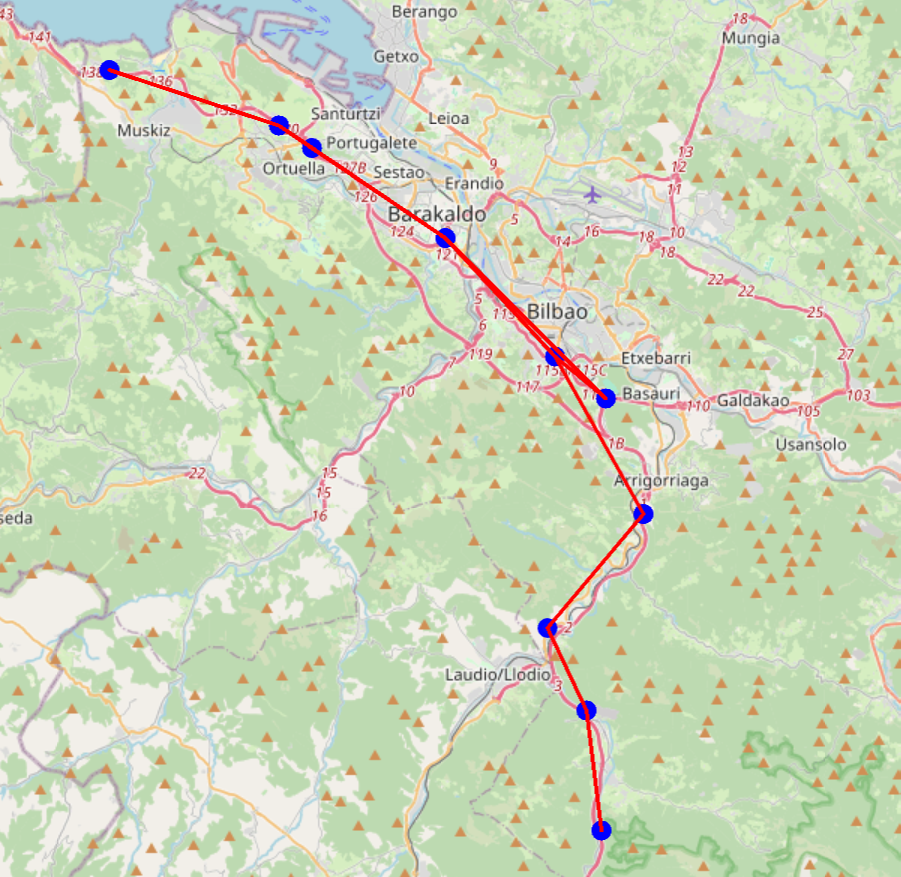
\includegraphics[width=0.7\linewidth]{includes/cap5/source_id_1_meters_mask.png}
	\caption{Distribución espacial de sensores para SourceId 1}
	\label{fig:sensores_sid1}
\end{figure}

La disposición de los sensores del SourceId 1, agrupados en puntos estratégicos específicos a lo largo de vías principales como se ve en la figura~\ref{fig:sensores_sid1}, permite al modelo Trafficformer aprovechar mejor las relaciones espaciales locales, favoreciendo su desempeño frente al modelo MLP.

\subsubsection*{Comparativa en sourceId 2}

La superioridad del modelo Trafficformer respecto al modelo MLP se acentúa aún más en los datos del sourceId 2. Como se observa en las figuras~\ref{fig:curvas_sid2_mlp} y \ref{fig:curvas_sid2_trafficformer}, Trafficformer reduce considerablemente el MAE desde 31.017 hasta 5.832 y el RMSE desde 38.177 hasta 15.046. El $R^2$ mejora sustancialmente de 0.866 (MLP) hasta 0.982 (Trafficformer), indicando una capacidad notablemente superior para explicar la variabilidad en los datos.

Las curvas de entrenamiento muestran una convergencia estable y continua del modelo Trafficformer hasta la época 96, reflejando una adecuada selección de hiperparámetros que permitió una optimización profunda. El modelo MLP, en cambio, converge rápidamente en la época 30, mostrando potencialmente limitaciones en su capacidad para aprovechar plenamente el volumen y complejidad de los datos disponibles.

\begin{figure}[H]
	\centering
	\includegraphics[width=0.7\linewidth]{includes/cap5/source_id_2_meters_mask.png}
	\caption{Distribución espacial de sensores para SourceId 2}
	\label{fig:sensores_sid2}
\end{figure}

La amplia distribución geográfica de los sensores para SourceId 2, como se aprecia en la figura~\ref{fig:sensores_sid2}, permite al modelo Trafficformer capturar relaciones espaciales complejas, aspecto que el modelo MLP no puede explotar debido a su limitada capacidad para modelar dependencias espaciales.

\subsubsection*{Comparativa en sourceId 5}

Para la fuente sourceId 5, el modelo Trafficformer sigue mostrando una clara ventaja frente al modelo MLP. Según las figuras~\ref{fig:curvas_sid5_mlp} y \ref{fig:curvas_sid5_trafficformer}, se observa una mejora en todas las métricas principales. El MAE disminuye desde 213.850 hasta 175.975, y el RMSE desde 343.603 hasta 306.134. El valor $R^2$ presenta una mejora significativa, desde un negativo e inadecuado -1.797 hasta un aceptable 0.640 para Trafficformer.

Las curvas de entrenamiento revelan que Trafficformer converge rápidamente (época 29), mostrando que el mecanismo de atención espacial resulta particularmente efectivo en escenarios urbanos densos como el representado en esta fuente de datos.

\begin{figure}[H]
	\centering
	\includegraphics[width=0.7\linewidth]{includes/cap5/source_id_5_meters_mask.png}
	\caption{Distribución espacial de sensores para SourceId 5}
	\label{fig:sensores_sid5}
\end{figure}

La concentración urbana y la alta densidad espacial del SourceId 5, apreciable en la figura~\ref{fig:sensores_sid5}, generan complejas interacciones entre sensores cercanos. Esta configuración beneficia notablemente al modelo Trafficformer frente al MLP, que carece de mecanismos específicos para gestionar esta complejidad espacial.

\subsubsection*{Análisis comparativo de fuentes de datos}

Las características particulares de cada fuente de datos han ejercido una influencia importante en el desempeño de los modelos.

\paragraph{SourceId 1} Este conjunto posee un total de 386 sensores (meters), aunque estos se encuentran ubicados en unos pocos puntos estratégicos distribuidos linealmente a lo largo de vías principales, como se observa en la figura \ref{fig:sensores_sid1}. Dado que cada sensor representa un carril individual, existe una alta densidad espacial localizada en ciertas áreas críticas, pero una baja distribución geográfica. El dataset utilizado para el entrenamiento tiene una dimensionalidad de entrada de 14,828 ventanas temporales, con una longitud de secuencia (\texttt{seq\_len}) de 8 (ventanas de 4 horas). El tamaño del conjunto de entrenamiento es de 10,379, validación 2,980, y test 1,469. Esta configuración temporal amplia permite al modelo captar patrones dinámicos extendidos en el tiempo, siendo favorable para el mecanismo de atención espacial del modelo Trafficformer.

\paragraph{SourceId 2} La fuente de datos 2 presenta una distribución geográfica amplia y diversa, cubriendo exhaustivamente la red viaria de Bizkaia (figura \ref{fig:sensores_sid2}). Inicialmente se consideraron 520 sensores, aunque tras el filtrado por ausencia de datos, el número efectivo de sensores fue de 462. Esto implica una alta complejidad en términos de relaciones espaciales y diversidad de patrones de tráfico. El conjunto de entrenamiento está compuesto por 12,292 ventanas temporales, mientras que validación y test contienen 3,530 y 1,739 ventanas respectivamente. Para esta fuente se ha empleado una ventana temporal más reducida (\texttt{seq\_len} = 4, equivalentes a ventanas de 2 horas), debido a la mayor densidad y complejidad espacial. La máscara espacial generada revela numerosas conexiones entre sensores distantes, lo que beneficia significativamente al modelo Trafficformer gracias a su capacidad de capturar relaciones espaciales complejas mediante atención multi-cabezal.

\paragraph{SourceId 5} El tercer conjunto se caracteriza por una cobertura urbana densa, centrado en la ciudad de Bilbao (figura \ref{fig:sensores_sid5}). Aunque inicialmente existían 92 sensores, el filtrado redujo el número a 70. La distribución espacial en un entorno urbano tan concentrado genera relaciones espaciales complejas y altamente correlacionadas. El dataset dispone de 17,330 ventanas temporales, dividido en entrenamiento (12,131 ventanas), validación (3,483 ventanas) y test (1,716 ventanas). También se empleó una ventana de 2 horas (\texttt{seq\_len} = 4), facilitando al modelo capturar dinámicas urbanas rápidas. La máscara espacial evidencia la compleja red de interacciones espaciales entre sensores urbanos cercanos, circunstancia que nuevamente favorece al modelo Trafficformer debido a su capacidad innata para modelar dependencias espaciales y temporales simultáneamente.

Este análisis de fuentes de datos subraya la importancia del diseño experimental y la selección de ventanas temporales adecuadas a las particularidades de cada conjunto, reflejándose directamente en el rendimiento relativo de los modelos evaluados.

\subsubsection*{Síntesis y reflexión general}

La superioridad generalizada del modelo Trafficformer sobre MLP en las tres fuentes de datos analizadas se explica principalmente por la capacidad de capturar dependencias espaciales y temporales mediante el mecanismo de atención multi-cabezal. Esta capacidad es especialmente valiosa en contextos urbanos complejos (sourceId 5) y en redes de sensores extensas (sourceId 2), donde las relaciones entre los puntos de medida tienen gran relevancia.

La elección de hiperparámetros, como el tamaño del batch, learning rate, número de cabezas de atención, y dimensión de embedding, ha demostrado ser crítica en la optimización de Trafficformer. Los resultados muestran que valores intermedios o altos para \texttt{num\_heads} y \texttt{embedding\_dim} mejoran significativamente el rendimiento, validando lo observado en estudios previos del estado del arte \cite{trafficformer}.

Finalmente, el análisis pone de manifiesto que el modelo MLP presenta limitaciones inherentes a su arquitectura más simple, especialmente en contextos con fuertes correlaciones espaciales o temporales. El modelo Trafficformer, al incluir mecanismos avanzados de atención, proporciona mayor robustez y capacidad predictiva, alineándose con las tendencias recientes en la literatura científica sobre modelos Transformer aplicados a predicción del tráfico.

\subsection{Análisis avanzado de resultados por fuente de datos}
\label{sec:analisis_avanzado_resultados}

Además del análisis comparativo entre las arquitecturas y fuentes de datos realizado previamente, se ha llevado a cabo un análisis avanzado, complementario y exhaustivo, con el objetivo de identificar patrones específicos y posibles limitaciones de los modelos entrenados. Este análisis incluye gráficos específicos tales como la representación del error absoluto frente a los valores reales, series temporales comparativas para sensores individuales, mapas de errores y gráficos de distribución del error por sensor.

A continuación, se presentan las conclusiones más relevantes derivadas del análisis avanzado realizado para cada una de las fuentes de datos (\texttt{sourceId}). El detalle completo de las gráficas mencionadas está disponible en el \hyperref[anexo:analisis_avanzado]{Anexo~H}.

\paragraph{SourceId 1}
El análisis avanzado sobre la fuente de datos 1 muestra una adecuada capacidad predictiva global del modelo Trafficformer. El gráfico de dispersión (scatter plot) revela una fuerte correlación entre los valores predichos y los reales, con la mayoría de puntos cercanos a la diagonal. Sin embargo, el histograma de errores refleja la presencia de errores significativos en ciertas predicciones puntuales, lo que sugiere áreas específicas donde el modelo podría mejorar. El mapa de errores confirma visualmente que la mayoría de errores altos se concentran en puntos geográficos específicos (probablemente zonas críticas de tráfico o intersecciones complejas), lo que podría ser causado por factores no capturados completamente por el modelo.

\paragraph{SourceId 2}
En el caso del sourceId 2, se observa un excelente rendimiento del modelo Trafficformer, especialmente notable en el gráfico de dispersión y el histograma de errores, que muestran una alta concentración alrededor del valor real y errores generalmente bajos. Sin embargo, la distribución espacial del error representada en el mapa destaca algunas ubicaciones específicas con errores ligeramente mayores, posiblemente relacionadas con zonas periféricas o sensores más aislados, donde la densidad de datos disponibles para el entrenamiento fue inferior. Las series temporales para los mejores y peores sensores confirman que los mayores errores ocurren en contextos específicos, probablemente vinculados a eventos atípicos o patrones de tráfico inusuales.

\paragraph{SourceId 5}
Finalmente, la fuente de datos 5, que cubre una zona urbana densa (Bilbao), presenta una complejidad intrínseca mayor. Esto se evidencia en el gráfico de dispersión, donde se observa una mayor dispersión de los puntos respecto a la diagonal ideal, indicando predicciones menos precisas para determinados sensores urbanos. El histograma del error muestra una distribución más amplia, sugiriendo heterogeneidad en la capacidad predictiva del modelo según zonas específicas. La distribución espacial de los errores confirma que áreas urbanas densamente pobladas y congestionadas muestran consistentemente errores más elevados, un aspecto esperado dada la complejidad del tráfico urbano.

Este análisis avanzado permite concluir que, aunque el modelo Trafficformer muestra en general buenos resultados en todas las fuentes de datos, existe un margen significativo de mejora en escenarios específicos y complejos, tales como intersecciones críticas y áreas urbanas densas. Además, pone de manifiesto la importancia del análisis visual detallado para identificar oportunidades específicas de optimización en futuras iteraciones del modelo.

Las gráficas completas utilizadas para este análisis avanzado se encuentran detalladamente en el \hyperref[anexo:analisis_avanzado]{Anexo~H}.


\subsection{Limitaciones y validez de los experimentos}
\label{sec:limitaciones_validez}

\begin{comment}
	- Discusión sobre limitaciones técnicas, posibles sesgos, restricciones de hardware, tamaño de muestra, etc.
\end{comment}

Aunque los resultados obtenidos a lo largo de este trabajo demuestran una alta eficacia en la predicción del tráfico mediante las arquitecturas propuestas, es fundamental reconocer ciertas limitaciones inherentes a la investigación realizada, que deben considerarse al interpretar los resultados obtenidos y planificar futuras líneas de trabajo.

En primer lugar, existe una \textbf{limitación asociada al tamaño y representatividad de las muestras}. Aunque se han empleado datasets significativos con numerosos sensores distribuidos espacialmente, ciertas fuentes de datos (como el caso del \texttt{sourceId 1}) presentan una distribución espacial concentrada en pocos puntos estratégicos. Esto podría implicar una representación parcial del comportamiento general del tráfico en áreas menos monitorizadas o rutas secundarias.

En segundo lugar, los experimentos se han visto afectados por ciertas \textbf{restricciones técnicas y de hardware}. La necesidad de entrenar múltiples modelos complejos como Trafficformer, con elevados requerimientos computacionales, ha limitado la exploración exhaustiva del espacio de hiperparámetros, especialmente en lo relativo al número de capas, cabezas de atención o tamaño de embedding. Esta limitación técnica puede haber impedido obtener resultados aún más óptimos.

Otra limitación importante reside en la \textbf{posible presencia de sesgos en los datos originales}. Los datasets provienen de fuentes públicas (Gobierno Vasco, Diputación Foral de Bizkaia y Ayuntamiento de Bilbao), por lo que es posible que contengan sesgos derivados de errores instrumentales, pérdida de datos en algunos sensores o inconsistencias temporales en la recopilación de información. Estos sesgos pueden afectar la precisión y generalización de los modelos desarrollados.

Adicionalmente, el uso exclusivo de \textbf{variables numéricas y categóricas predefinidas} limita la capacidad del modelo para captar factores externos relevantes, como eventos específicos no registrados, cambios estacionales detallados o efectos socioeconómicos más amplios, que podrían mejorar la precisión y robustez del modelo.

Por último, la \textbf{validez externa y generalización} de los resultados está condicionada al contexto específico de la provincia de Bizkaia. Aunque la metodología aplicada es escalable y transferible a otros contextos urbanos, es necesario realizar experimentos adicionales para confirmar que los modelos desarrollados mantienen su rendimiento en otras regiones con diferentes características geográficas, culturales y económicas.

Estas limitaciones deben ser tomadas como puntos de partida para futuras investigaciones, enfocadas hacia la mejora de los modelos y la inclusión de nuevas fuentes de datos y técnicas que puedan aumentar la robustez y generalización del sistema propuesto.



	\clearpage
	\section*{Conclusiones y trabajo futuro}
\label{sec:conclusiones}
\addcontentsline{toc}{section}{Conclusiones y trabajo futuro}

%
% Para citar: 
% 	(ver Sección~\ref{sec:dataset_arquitectura})
% 	como se describe en la Sección~\nameref{sec:dataset_arquitectura})
%

Este capítulo sintetiza los hallazgos principales derivados del desarrollo y evaluación de los modelos propuestos en este trabajo fin de máster. Se presentan primero las conclusiones fundamentales del estudio, seguidas por recomendaciones y propuestas específicas para futuras investigaciones.

\subsection{Conclusiones}

El desarrollo de este trabajo ha permitido abordar con éxito el objetivo principal planteado inicialmente: diseñar, implementar y evaluar modelos de predicción del tráfico vehicular mediante técnicas avanzadas de aprendizaje profundo, destacando especialmente la arquitectura \texttt{Trafficformer} basada en Transformers con atención espacial.

La comparación entre \texttt{MLP} y \texttt{Trafficformer} ha demostrado la clara superioridad del segundo en los tres contextos evaluados (sourceIds 1, 2 y 5). Trafficformer logró resultados significativamente mejores en métricas clave como MAE, RMSE y $R^2$, validando así su capacidad para explotar eficazmente dependencias espaciales y temporales, especialmente en escenarios complejos con alta densidad y distribución espacial.

La metodología de experimentación exhaustiva permitió identificar combinaciones óptimas de hiperparámetros (tamaño de ventana temporal, número de cabezas de atención, tamaño de embedding, entre otros), destacando la importancia crítica del ajuste adecuado de estos parámetros para obtener un rendimiento óptimo del modelo.

Asimismo, la utilización de la plataforma \textit{Weights & Biases} ha resultado fundamental para asegurar la reproducibilidad, transparencia y análisis riguroso de los experimentos, proporcionando un seguimiento detallado y sistemático del proceso de entrenamiento y evaluación.

No obstante, el trabajo ha revelado diversas limitaciones, principalmente relacionadas con la representatividad espacial de las fuentes de datos, restricciones técnicas de hardware, posibles sesgos en los datos y limitaciones en la generalización externa. Estas limitaciones representan oportunidades claras para futuros desarrollos y mejoras.

\subsection{Trabajo Futuro}

De cara a futuras investigaciones, se identifican diversas líneas de trabajo que permitirían mejorar aún más los resultados obtenidos:

\begin{itemize}
	\item \textbf{Ampliación de datos y fuentes adicionales}: Incorporar nuevos conjuntos de datos provenientes de otras regiones o ciudades, así como otras variables exógenas no consideradas, para mejorar la generalización y robustez del modelo.
	\item \textbf{Optimización y escalado del modelo}: Realizar experimentos con infraestructuras computacionales más potentes (por ejemplo, GPU de alto rendimiento o clústeres en la nube), lo que permitiría profundizar en la exploración de hiperparámetros y probar arquitecturas más complejas. Para ello, en el proyecto actual se provee de una implementación lista para usar en Amazon Web Services.
	\item \textbf{Técnicas avanzadas de tratamiento de datos}: Evaluar el impacto de estrategias más avanzadas de imputación de datos, tratamiento de valores atípicos, y técnicas de aprendizaje auto-supervisado que podrían mejorar la calidad y representatividad de los datasets empleados.
	\item \textbf{Evaluación en tiempo real y despliegue operativo}: Desarrollar un sistema integrado capaz de realizar predicciones en tiempo real, desplegado en un entorno operativo real, permitiendo validar su utilidad práctica y detectar oportunidades adicionales de mejora.
	\item \textbf{Interpretabilidad y explicabilidad}: Implementar técnicas adicionales que aumenten la interpretabilidad de los modelos desarrollados, facilitando la comprensión y justificación de las decisiones tomadas por el sistema.
	\item \textbf{Integración de otros modelos avanzados}: Explorar modelos complementarios como Graph Neural Networks (GNNs) o modelos híbridos que podrían aprovechar aún más las estructuras espaciales complejas presentes en los datos de tráfico.
\end{itemize}

En conclusión, este TFM establece una sólida base metodológica y técnica para futuros trabajos en predicción de tráfico, y destaca la capacidad de los modelos basados en Transformers, particularmente Trafficformer, para abordar eficazmente desafíos de alta complejidad espacial y temporal.



	\clearpage
	
	\clearpage
	\printglossary[type=\acronymtype,title={Acrónimos y Abreviaturas}]
	\printglossary
	\glsaddallunused

	\clearpage
	\phantomsection %Insertamos ancla en la bibliografía para hipervínculo
	\begin{flushleft}
		%Visualizar bibliografía con notice incluida la no citada
		\nocite{*}
		\bibliographystyle{apacite}
		\bibliography{recursos/bibliografia}
	\end{flushleft}

	\clearpage
	\appendix
	
	\section*{Anexo A – Descripción de sensores meteorológicos}
\label{anexo:sensores}
\addcontentsline{toc}{section}{Anexo A – Descripción de sensores meteorológicos}

En este anexo se presenta un listado exhaustivo de los sensores meteorológicos utilizados en la construcción del dataset. Cada sensor cuenta con un identificador único, una abreviatura técnica y una descripción textual de la variable que mide. Estos sensores provienen de estaciones automáticas distribuidas en la CAPV, y sus mediciones son fundamentales para enriquecer los \texttt{MobilitySnapshot} con información climática contextual.

La codificación y nomenclatura de los sensores meteorológicos responde al estándar empleado por Euskalmet, el cual está documentado en su catálogo de abreviaturas técnicas de tipo de sensor~\cite{sensorTypeAbbrv}.

\vspace{1em}

\begin{longtable}{|c|l|p{8.5cm}|}
	\hline
	\textbf{ID} & \textbf{Nombre} & \textbf{Descripción} \\
	\hline
	\endfirsthead
	\hline
	\textbf{ID} & \textbf{Nombre} & \textbf{Descripción} \\
	\hline
	\endhead
	\hline
	\endfoot
	
	12 & Dir.Med & Dirección media del viento en grados (º) \\
	14 & Vel.Max & Racha máxima del viento horizontal en km/h \\
	16 & Sig.Vel & Sigma de la velocidad del viento en km/h \\
	17 & Sig.Dir & Sigma de la dirección del viento en grados (º) \\
	18 & Cub.Vto & Velocidad cúbica media del viento en Dm/s³ \\
	21 & Tem.Aire & Temperatura del aire en ºC \\
	31 & Humedad & Humedad relativa del aire en \% \\
	40 & Precip. & Precipitación acumulada en mm o l/m² \\
	50 & Presión & Presión atmosférica en milibares (mb) \\
	60 & Nivel 1 & Nivel de lámina de agua en metros (m) \\
	61 & Nivel 2 & Nivel de lámina de agua en metros (m) \\
	70 & Irradia. & Irradiancia solar global en w/m² \\
	90 & Tem.Agua & Temperatura del agua en ºC \\
	91 & Oxígeno & Oxígeno disuelto en ppm \\
	92 & pH & pH del agua \\
	93 & Conduct. & Conductividad del agua en μS \\
	94 & Amonio & Amonio en mg/l \\
	95 & Turbidez & Turbidez del agua en NTU \\
	96 & Redox. & Potencial redox del agua en mV \\
	97 & Mat.Org. & Materia orgánica medida como demanda de oxígeno \\
	11 & VelMed & Velocidad media del viento en km/h \\
	22 & Tem.Sue & Temperatura del suelo en ºC \\
	B0 & Visibili & Visibilidad en metros \\
	B1 & Nivelm 1 & Nivel del mar (sensor 1) en metros \\
	B2 & Nivelm 2 & Nivel del mar (sensor 2) en metros \\
	B3 & Ola Med & Altura media de ola en metros \\
	B4 & Ola Max & Altura máxima de ola en metros \\
	B5 & Ola Sig & Altura significante de ola en metros \\
	B6 & Ola Per & Periodo de oleaje en segundos \\
	B7 & Pre MSP & Presión hidrostática MSP en hPa \\
	B8 & Pre LSP & Presión hidrostática LSP en hPa \\
	B9 & Vel Cor & Velocidad de corriente en cm/s \\
	BA & Dir Cor & Dirección de la corriente en grados (º) \\
	BB & Tem Mar & Temperatura del agua del mar en ºC \\
	BC & Tem Ter & Temperatura termistor en ºC \\
	BD & Ola Sig2 & Altura significante de ola (variante) en metros \\
	72 & Rad.Refl & Radiación solar reflejada en w/m² \\
	73 & Rad.UV & Radiación UV en J/m² h \\
	\hline
\end{longtable}
	\clearpage
	\section*{Anexo B – Código fuente del generador de snapshots}
\label{anexo:snapshot_generator}
\addcontentsline{toc}{section}{Anexo B – Código fuente del generador de snapshots}

A continuación se presenta el código fuente completo de la clase \texttt{MobilitySnapshotGeneratorService}, responsable de generar las instancias de \texttt{MobilitySnapshot} mediante la integración de datos de tráfico, meteorología e incidencias.

\begin{lstlisting}[language=Kotlin, caption={Clase MobilitySnapshotGeneratorService}]
	package es.joninx.tfm.dc.service
	
	import es.joninx.tfm.dc.builder.dataset.MobilitySnapshotBuilder
	import es.joninx.tfm.dc.config.Cfg
	import es.joninx.tfm.dc.repository.meteo.ReadingXmlRepository
	import es.joninx.tfm.dc.repository.meteo.StationRepository
	import es.joninx.tfm.dc.repository.traffic.FlowRepository
	import es.joninx.tfm.dc.repository.traffic.IncidenceRepository
	import es.joninx.tfm.dc.repository.traffic.MeterRepository
	import es.joninx.tfm.dc.util.DateTimeUtils
	import org.apache.logging.log4j.LogManager
	import org.apache.logging.log4j.Logger
	import org.springframework.stereotype.Service
	import java.time.Duration
	import java.time.LocalDateTime
	
	@Service
	class MobilitySnapshotGeneratorService(
		private val cfg: Cfg,
	
		private val snapshotBuilder: MobilitySnapshotBuilder,
		private val snapshotPersistenceService: MobilitySnapshotPersistenceService,
		private val flowRepository: FlowRepository,
		private val meterRepository: MeterRepository,
		private val incidenceRepository: IncidenceRepository,
		private val stationRepository: StationRepository,
		private val meteoReadingsRepository: ReadingXmlRepository,
	) {
		
		/**
		* Mapa cache: meterId → stationId
		*/
		private val meterToStationCache = mutableMapOf<String, String>()
		
		fun getNearestStationId(meterId: String, latitude: Double, longitude: Double): String? {
			// ¿Ya lo tenemos cacheado?
			meterToStationCache[meterId]?.let {
				log.debug("Cache HIT: meterId=$meterId → stationId=$it")
				return it
			}
			
			// Si no, buscamos la estación más cercana
			val nearestStation = stationRepository.findNearestStation(
			longitude = longitude,
			latitude = latitude,
			maxDistanceMeters = cfg.algorithm.maxDistanceToStation
			).blockFirst() ?: return null
			
			meterToStationCache[meterId] = nearestStation.stationId
			log.debug("Cache MISS: meterId=$meterId → stationId=${nearestStation.stationId}")
			return nearestStation.stationId
		}
		
		fun generateSnapshots(
			sourceIds: List<String>,
			startDate: LocalDateTime,
			endDate: LocalDateTime,
			batchSize: Int = 500
		) {
			log.debug("Comenzando generación de MobilitySnapshots para sourceIds=${sourceIds.joinToString(",")}, fechas entre '${DateTimeUtils.format(startDate)}' y '${DateTimeUtils.format(endDate)}'")
			
			val meters = meterRepository.findAllBySourceIdIn(sourceIds)
			.collectMap { it.meterId }
			.block() ?: emptyMap()
			
			val intervals = generateIntervals(startDate, endDate, cfg.algorithm.timeWindowDuration)
			var totalSnapshots = 0
			
			intervals.forEachIndexed { idx, (intervalStart, intervalEnd) ->
				val flows = flowRepository.findAllBySourceIdInAndDateTimeBetweenQuery(
				sourceIds, intervalStart, intervalEnd
				).collectList().block() ?: emptyList()
				
				val groupedByMeter = flows.groupBy { it.meterId }
				
				val snapshots = groupedByMeter.mapNotNull { (meterId, flowList) ->
					val meter = meters[meterId]
					if (meter != null && flowList.isNotEmpty()) {
						val totalVehiclesSum = flowList.sumOf { it.totalVehicles.toIntOrNull() ?: 0 }
						
						// Obtener incidencias para el intervalo
						val latitude = meter.latitude
						val longitude = meter.longitude
						
						// Busca incidencias cercanas y activas
						val incidences = incidenceRepository
						.findIncidencesNearAndActive(
						longitude, latitude, cfg.algorithm.maxDistanceToIncidences,
						intervalStart, intervalEnd
						)
						.collectList()
						.block() ?: emptyList()
						
						// Meteo
						val nearestStationId = getNearestStationId(
						meterId = meterId,
						latitude = latitude,
						longitude = longitude
						)
						val meteoReadings = if (nearestStationId != null) {
							meteoReadingsRepository.findReadingsByStationIdAndDateTimeBetween(
							stationId = nearestStationId,
							windowStart = intervalStart,
							windowEnd = intervalEnd
							).collectList().block() ?: emptyList()
						} else emptyList()
						
						log.debug("Intervalo '${DateTimeUtils.format(intervalStart)}' → '${DateTimeUtils.format(intervalEnd)}' | meterId=$meterId | numFlows=${flowList.size} | totalVehiclesSum=$totalVehiclesSum | totalIncidences=${incidences.size} |meteoReadings=${meteoReadings.size}")
						snapshotBuilder.fromGroupedFlows(
						flows = flowList,
						meter = meter,
						windowStartDateTime = intervalStart,
						windowEndDateTime = intervalEnd,
						totalVehicles = totalVehiclesSum,
						incidences = incidences,
						meteoReadings = meteoReadings,
						)
					} else {
						if (meter == null) {
							log.warn("MeterId=$meterId no encontrado en meterMap para ventana '${DateTimeUtils.format(intervalStart)}' → '${DateTimeUtils.format(intervalEnd)}'")
						} else {
							log.warn("No hay flows para meterId=$meterId en ventana '${DateTimeUtils.format(intervalStart)}' → '${DateTimeUtils.format(intervalEnd)}'")
						}
						null
					}
				}
				
				// Guardar por lotes
				snapshots.chunked(batchSize).forEach { batch ->
					snapshotPersistenceService.saveBatch(batch).block()
					log.debug("Batch guardado para intervalo $intervalStart → $intervalEnd (${batch.size} snapshots)")
				}
				totalSnapshots += snapshots.size
				
				if ((idx + 1) % 24 == 0) { // Cada 12 horas
					log.debug("Progreso: ${idx + 1} de ${intervals.size} intervalos procesados, $totalSnapshots snapshots generados.")
				}
			}
			
			log.debug("Generación de MobilitySnapshots finalizada. Total snapshots: $totalSnapshots")
		}
		
		// Utilidad para generar ventanas de 30 minutos (la misma que antes)
		fun generateIntervals(start: LocalDateTime, end: LocalDateTime, step: Duration): List<Pair<LocalDateTime, LocalDateTime>> {
			val intervals = mutableListOf<Pair<LocalDateTime, LocalDateTime>>()
			var current = start
			while (current.isBefore(end)) {
				val next = current.plus(step)
				intervals.add(Pair(current, if (next.isBefore(end)) next else end))
				current = next
			}
			return intervals
		}
		
		companion object {
			val log: Logger = LogManager.getLogger(this::class.java)
		}
		
	}
\end{lstlisting}
	\clearpage
	\section*{Anexo C – Plantilla de infraestructura para AWS}
\label{anexo:plantilla_aws}
\addcontentsline{toc}{section}{Anexo C – Plantilla de infraestructura para AWS}

Con el objetivo de permitir la escalabilidad y entrenamiento de los modelos desarrollados en la nube, se ha preparado una plantilla de infraestructura como código en formato \texttt{YAML}, siguiendo el estándar \texttt{AWS CloudFormation}.

Esta plantilla permite desplegar de forma automática una instancia con aceleración por GPU, almacenamiento persistente y conexión segura a la base de datos local mediante VPN. Aunque no ha sido necesario su uso durante el desarrollo del presente trabajo, se considera un componente valioso para futuras ejecuciones de alto rendimiento o despliegues remotos. La plantilla está pensada para ser lanzada directamente desde la consola de AWS o mediante herramientas como \texttt{AWS SAM} o \texttt{AWS CLI}.

\begin{lstlisting}[language=yaml, caption={Plantilla CloudFormation utilizada para el despliegue de entorno de entrenamiento}, label={lst:template_yaml}, {recursos/template.yaml}]

  AWSTemplateFormatVersion: '2010-09-09'
  Description: EC2 g5.xlarge Ubuntu 24.04 DLAMI GPU con volumen persistente y WireGuard
	
  Parameters:
    KeyName:
      Type: AWS::EC2::KeyPair::KeyName
      Default: joninx
    WireguardConfBucket:
      Type: String
      Default: tfm-jon-trafficformer
    WireguardConfKey:
      Type: String
      Default: wireguard/joninx.conf

  Resources:
    VPC:
      Type: AWS::EC2::VPC
      Properties:
        CidrBlock: 10.100.0.0/16
        Tags: [{Key: Name, Value: tfm}]
    
    InternetGateway: {Type: AWS::EC2::InternetGateway}
    AttachGateway:
      Type: AWS::EC2::VPCGatewayAttachment
      Properties:
        VpcId: !Ref VPC
        InternetGatewayId: !Ref InternetGateway
    
    PublicSubnet:
      Type: AWS::EC2::Subnet
      Properties:
        VpcId: !Ref VPC
        CidrBlock: 10.100.1.0/24
        MapPublicIpOnLaunch: true
        AvailabilityZone: !Select [0, !GetAZs '']
        Tags: [{Key: Name, Value: tfm}]
    
    RouteTable:
      Type: AWS::EC2::RouteTable
      Properties:
        VpcId: !Ref VPC
        Tags: [{Key: Name, Value: tfm}]
    PublicRoute:
      Type: AWS::EC2::Route
      DependsOn: AttachGateway
      Properties:
        RouteTableId: !Ref RouteTable
        DestinationCidrBlock: 0.0.0.0/0
        GatewayId: !Ref InternetGateway
    RouteTableAssoc:
      Type: AWS::EC2::SubnetRouteTableAssociation
      Properties:
        SubnetId: !Ref PublicSubnet
        RouteTableId: !Ref RouteTable

    SecurityGroup:
      Type: AWS::EC2::SecurityGroup
      Properties:
        GroupDescription: SSH access
        VpcId: !Ref VPC
        SecurityGroupIngress:
          - IpProtocol: tcp
            FromPort: 22
            ToPort: 22
            CidrIp: 0.0.0.0/0
        Tags: [{Key: Name, Value: tfm}]
  
  EC2InstanceProfile:
    Type: AWS::IAM::InstanceProfile
    Properties:
      Roles: [!Ref EC2S3AccessRole]
  
  EC2S3AccessRole:
    Type: AWS::IAM::Role
    Properties:
      AssumeRolePolicyDocument:
        Version: "2012-10-17"
        Statement:
          - Effect: Allow
            Principal: {Service: ec2.amazonaws.com}
            Action: sts:AssumeRole
      Policies:
        - PolicyName: S3WGAccess
          PolicyDocument:
          Version: "2012-10-17"
          Statement:
            - Effect: Allow
              Action: s3:GetObject
              Resource: !Sub arn:aws:s3:::${WireguardConfBucket}/${WireguardConfKey}
              
  EC2DataVolume:
    Type: AWS::EC2::Volume
    Properties:
      AvailabilityZone: !Select [0, !GetAZs '']
      Size: 200
      VolumeType: gp3
      Encrypted: true
      Tags: [{Key: Name, Value: tfm}]
  
  EC2Instance:
    Type: AWS::EC2::Instance
    Properties:
      InstanceType: g5.2xlarge
      KeyName: !Ref KeyName
      SubnetId: !Ref PublicSubnet
      SecurityGroupIds: [!Ref SecurityGroup]
      IamInstanceProfile: !Ref EC2InstanceProfile
      BlockDeviceMappings:
        - DeviceName: /dev/sda1
          Ebs:
          VolumeSize: 60
          VolumeType: gp3
          DeleteOnTermination: true
      ImageId: !Sub "{{resolve:ssm:/aws/service/deeplearning/ami/x86_64/base-oss-nvidia-driver-gpu-ubuntu-24.04/latest/ami-id}}"
      Tags: [{Key: Name, Value: tfm}]
      UserData:
        Fn::Base64: !Sub |
          #!/bin/bash
          set -eux
          apt-get update -y
          apt-get upgrade -y
          # Instala Python 3.13 desde deadsnakes PPA (o desde source si necesario)
          if ! python3.13 --version 2>/dev/null; then
          apt-get install -y software-properties-common
          add-apt-repository ppa:deadsnakes/ppa -y
          apt-get update -y
          apt-get install -y python3.13 python3.13-venv python3.13-distutils
          fi
          # Configura python3 para que apunte a 3.13 por defecto
          update-alternatives --install /usr/bin/python3 python3 /usr/bin/python3.13 2
          update-alternatives --set python3 /usr/bin/python3.13
          # Instala pip y venv para 3.13 si no están
          curl -sS https://bootstrap.pypa.io/get-pip.py | python3.13
          
          # Python 3.13 alternativo
          update-alternatives --install /usr/bin/python3 python3 /usr/bin/python3.13 2
          
          # Instala wireguard y awscli
          apt-get install -y wireguard awscli
          
          # WireGuard config
          aws s3 cp s3://${WireguardConfBucket}/${WireguardConfKey} /etc/wireguard/wg0.conf
          chmod 600 /etc/wireguard/wg0.conf
          systemctl enable wg-quick@wg0 && systemctl start wg-quick@wg0
          
          # Attach, format & mount data volume
          mkfs.ext4 -F /dev/xvdb || true
          mkdir -p /mnt/tfmdata
          mount /dev/xvdb /mnt/tfmdata
          echo '/dev/xvdb /mnt/tfmdata ext4 defaults,nofail 0 2' >> /etc/fstab
          chown ubuntu:ubuntu /mnt/tfmdata
  
  AttachDataVolume:
    Type: AWS::EC2::VolumeAttachment
    Properties:
      Device: /dev/xvdb
      InstanceId: !Ref EC2Instance
      VolumeId: !Ref EC2DataVolume
  
  Outputs:
    PublicIP:
      Description: "EC2 Public IP"
      Value: !GetAtt EC2Instance.PublicIp
\end{lstlisting}
	\clearpage
	\section*{Anexo D – Código fuente de la arquitectura Trafficformer}
\label{anexo:codigo_trafficformer}
\addcontentsline{toc}{section}{Anexo D – Código fuente de la arquitectura Trafficformer}

A continuación se presenta el código fuente completo de la arquitectura \texttt{Trafficformer}, implementada en Python y utilizada como modelo principal en el presente trabajo. El código está debidamente documentado mediante docstrings, y ha sido diseñado con una estructura modular que facilita su reutilización y extensión.

\lstinputlisting[language=Python, basicstyle=\footnotesize\ttfamily, breaklines=true]{recursos/anexo_d_trafficformer.py}
	\clearpage
	\section*{Anexo E – Listado detallado de combinaciones por modelo}
\label{anexo:combinaciones_exp}
\addcontentsline{toc}{section}{Anexo E – Listado detallado de combinaciones por modelo}

Este anexo recoge todas las combinaciones de hiperparámetros evaluadas durante los experimentos de entrenamiento, tanto para el modelo base \texttt{MLP} como para el modelo avanzado \texttt{Trafficformer}. Se han definido y ejecutado un total de 120 configuraciones distintas, distribuidas de forma equitativa entre tres fuentes de datos (\texttt{sourceId} 1, 2 y 5). Cada configuración representa una combinación específica de parámetros como la longitud de la secuencia de entrada, tasa de aprendizaje, tamaño del batch, número de capas, dimensiones del embedding, entre otros.

\subsubsection*{MLP (por sourceId)}

En el caso del modelo \texttt{MLP}, se han explorado ocho combinaciones por cada \texttt{sourceId}, con variaciones en tres hiperparámetros clave: la longitud de la ventana temporal (\texttt{seq\_len}), la tasa de aprendizaje (\texttt{learning\_rate}) y el tamaño del batch (\texttt{batch\_size}). Esto se ve en la Tabla~\ref{tab:mlp_combinaciones}.

\begin{table}[H]
	\centering
	\caption{Combinaciones evaluadas para el modelo MLP (por cada \texttt{sourceId})}
	\label{tab:mlp_combinaciones}
	\begin{tabularx}{\textwidth}{>{\raggedleft\arraybackslash}p{1cm} >{\centering\arraybackslash}p{2.5cm} >{\centering\arraybackslash}p{3cm} >{\centering\arraybackslash}p{3cm}}
		\toprule
		\textbf{NN} & \textbf{seq\_len} & \textbf{learning\_rate} & \textbf{batch\_size} \\
		\midrule
		01 & 4 & 0.001  & 32 \\
		02 & 4 & 0.001  & 64 \\
		03 & 4 & 0.0005 & 32 \\
		04 & 4 & 0.0005 & 64 \\
		05 & 8 & 0.001  & 32 \\
		06 & 8 & 0.001  & 64 \\
		07 & 8 & 0.0005 & 32 \\
		08 & 8 & 0.0005 & 64 \\
		\bottomrule
	\end{tabularx}
\end{table}

\subsubsection*{Trafficformer (por sourceId)}

En el caso del modelo \texttt{Trafficformer}, se han diseñado 32 combinaciones por cada \texttt{sourceId}, contemplando una variedad mucho mayor de hiperparámetros. Las variables analizadas incluyen además de las anteriores, el número de cabezas de atención (\texttt{num\_heads}), la dimensión del embedding (\texttt{embedding\_dim}), el número de capas (\texttt{num\_layers}) y la dimensión oculta del bloque feedforward (\texttt{ff\_hidden\_dim}). Estas combinaciones permiten evaluar el impacto de cada configuración sobre la capacidad de generalización y aprendizaje del modelo. Esto se ve en la Tabla~\ref{tab:trafficformer_combinaciones}.

\begin{table}[H]
	\centering
	\caption{Combinaciones evaluadas para el modelo Trafficformer (por cada \texttt{sourceId})}
	\label{tab:trafficformer_combinaciones}
	\begin{tabularx}{\textwidth}{>{\raggedleft\arraybackslash}p{0.7cm} >{\centering\arraybackslash}p{1cm} >{\centering\arraybackslash}p{1.6cm} >{\centering\arraybackslash}p{1.6cm} >{\centering\arraybackslash}p{1.3cm} >{\centering\arraybackslash}p{1.8cm} >{\centering\arraybackslash}p{1.3cm} >{\centering\arraybackslash}p{2cm}}
		\toprule
		\textbf{NN} & \textbf{seq\_len} & \textbf{learning\_rate} & \textbf{batch\_size} & \textbf{num\_heads} & \textbf{embedding\_dim} & \textbf{num\_layers} & \textbf{ff\_hidden\_dim} \\
		\midrule
		01 & 4 & 0.001 & 32 & 4 & 64 & 4 & 256 \\
		02 & 4 & 0.001 & 32 & 4 & 64 & 6 & 512 \\
		03 & 4 & 0.001 & 32 & 8 & 128 & 4 & 256 \\
		04 & 4 & 0.001 & 32 & 8 & 128 & 6 & 512 \\
		05 & 4 & 0.001 & 64 & 4 & 64 & 4 & 256 \\
		06 & 4 & 0.001 & 64 & 4 & 64 & 6 & 512 \\
		07 & 4 & 0.001 & 64 & 8 & 128 & 4 & 256 \\
		08 & 4 & 0.001 & 64 & 8 & 128 & 6 & 512 \\
		09 & 4 & 0.0005 & 32 & 4 & 64 & 4 & 256 \\
		10 & 4 & 0.0005 & 32 & 4 & 64 & 6 & 512 \\
		11 & 4 & 0.0005 & 32 & 8 & 128 & 4 & 256 \\
		12 & 4 & 0.0005 & 32 & 8 & 128 & 6 & 512 \\
		13 & 4 & 0.0005 & 64 & 4 & 64 & 4 & 256 \\
		14 & 4 & 0.0005 & 64 & 4 & 64 & 6 & 512 \\
		15 & 4 & 0.0005 & 64 & 8 & 128 & 4 & 256 \\
		16 & 4 & 0.0005 & 64 & 8 & 128 & 6 & 512 \\
		17 & 8 & 0.001 & 32 & 4 & 64 & 4 & 256 \\
		18 & 8 & 0.001 & 32 & 4 & 64 & 6 & 512 \\
		19 & 8 & 0.001 & 32 & 8 & 128 & 4 & 256 \\
		20 & 8 & 0.001 & 32 & 8 & 128 & 6 & 512 \\
		21 & 8 & 0.001 & 64 & 4 & 64 & 4 & 256 \\
		22 & 8 & 0.001 & 64 & 4 & 64 & 6 & 512 \\
		23 & 8 & 0.001 & 64 & 8 & 128 & 4 & 256 \\
		24 & 8 & 0.001 & 64 & 8 & 128 & 6 & 512 \\
		25 & 8 & 0.0005 & 32 & 4 & 64 & 4 & 256 \\
		26 & 8 & 0.0005 & 32 & 4 & 64 & 6 & 512 \\
		27 & 8 & 0.0005 & 32 & 8 & 128 & 4 & 256 \\
		28 & 8 & 0.0005 & 32 & 8 & 128 & 6 & 512 \\
		29 & 8 & 0.0005 & 64 & 4 & 64 & 4 & 256 \\
		30 & 8 & 0.0005 & 64 & 4 & 64 & 6 & 512 \\
		31 & 8 & 0.0005 & 64 & 8 & 128 & 4 & 256 \\
		32 & 8 & 0.0005 & 64 & 8 & 128 & 6 & 512 \\
		\bottomrule
	\end{tabularx}
\end{table}
	\clearpage
	\section*{Anexo F – Resultados detallados de los 120 experimentos}
\label{anexo:resultados_exp}
\addcontentsline{toc}{section}{Anexo F – Resultados detallados de los 120 experimentos}

Este anexo recoge el resultado completo de los 120 experimentos de entrenamiento realizados, abarcando diferentes modelos, fuentes de datos y combinaciones de hiperparámetros. Se incluyen, para cada experimento, los valores principales de las métricas obtenidas en validación y test: \texttt{loss}, \texttt{mae}, \texttt{rmse}, \texttt{mape} y \texttt{r2}, además de la epoch de mejor resultado. 

La tabla siguiente muestra la información relevante de cada experimento, agrupando por fuente de datos (\texttt{sourceId}) y modelo (\texttt{model}).

\begin{center}
	\scriptsize
	\setlength{\extrarowheight}{0.5pt}
	\begin{tabularx}{\textwidth}{>{\raggedleft\arraybackslash}p{0.4cm} >{\centering\arraybackslash}p{0.45cm} >{\centering\arraybackslash}X >{\centering\arraybackslash}p{0.6cm} >{\centering\arraybackslash}p{1.1cm} >{\centering\arraybackslash}p{1.1cm} >{\centering\arraybackslash}p{1.1cm} >{\centering\arraybackslash}p{1.1cm} >{\centering\arraybackslash}p{0.9cm} >{\centering\arraybackslash}p{1.1cm} >{\centering\arraybackslash}p{1.1cm} >{\centering\arraybackslash}p{1.1cm} >{\centering\arraybackslash}p{1.1cm} >{\centering\arraybackslash}p{0.9cm}}
		\caption{Métricas principales de los 120 experimentos realizados (validación y test).} \\
		\toprule
		\textbf{ID} & \textbf{Src} & \textbf{Modelo} & \textbf{Ep} & \textbf{Val Loss} & \textbf{Val MAE} & \textbf{Val RMSE} & \textbf{Val MAPE} & \textbf{Val R2} & \textbf{Test Loss} & \textbf{Test MAE} & \textbf{Test RMSE} & \textbf{Test MAPE} & \textbf{Test R2} \\
		\midrule
		\endfirsthead
		
		\multicolumn{14}{l}%
		{{\bfseries \tablename\ \thetable{} -- continuación de la página anterior}} \\
		\toprule
		\textbf{ID} & \textbf{Src} & \textbf{Modelo} & \textbf{Ep} & \textbf{Val Loss} & \textbf{Val MAE} & \textbf{Val RMSE} & \textbf{Val MAPE} & \textbf{Val R2} & \textbf{Test Loss} & \textbf{Test MAE} & \textbf{Test RMSE} & \textbf{Test MAPE} & \textbf{Test R2} \\
		\midrule
		\endhead
		
		\bottomrule
		\multicolumn{14}{r}{{Continúa en la siguiente página}} \\
		\endfoot
		
		\bottomrule
		\endlastfoot
		1 & 1 & MLP & 21 & 0.002531 & 0.037882 & 0.045857 & 21.077439 & 0.964011 & 0.002628 & 0.038794 & 0.046621 & 21.545246 & 0.962530 \\
		2 & 1 & MLP & 40 & 0.002647 & 0.038681 & 0.046977 & 21.463618 & 0.962054 & 0.002772 & 0.039857 & 0.047914 & 22.135354 & 0.960350 \\
		3 & 1 & MLP & 25 & 0.002478 & 0.037261 & 0.045537 & 20.822926 & 0.964684 & 0.002567 & 0.038133 & 0.046172 & 21.283347 & 0.963350 \\
		4 & 1 & MLP & 38 & 0.002452 & 0.037038 & 0.045358 & 20.710834 & 0.965002 & 0.002542 & 0.037919 & 0.045987 & 21.163511 & 0.963680 \\
		5 & 1 & MLP & 32 & 0.002467 & 0.037130 & 0.045422 & 20.756244 & 0.964849 & 0.002555 & 0.037989 & 0.046049 & 21.184368 & 0.963583 \\
		6 & 1 & MLP & 15 & 0.002509 & 0.037486 & 0.045644 & 20.920890 & 0.964370 & 0.002596 & 0.038565 & 0.046443 & 21.390472 & 0.962979 \\
		7 & 1 & MLP & 33 & 0.002493 & 0.037332 & 0.045515 & 20.815909 & 0.964623 & 0.002584 & 0.038420 & 0.046330 & 21.345234 & 0.963147 \\
		8 & 1 & MLP & 39 & 0.002462 & 0.037053 & 0.045375 & 20.709663 & 0.964982 & 0.002554 & 0.037997 & 0.046056 & 21.186427 & 0.963570 \\
		9 & 1 & Trafficformer & 71 & 0.001816 & 0.031694 & 0.041054 & 19.023583 & 0.971024 & 0.001919 & 0.032790 & 0.041963 & 19.617563 & 0.969697 \\
		10 & 1 & Trafficformer & 62 & 0.001847 & 0.031983 & 0.041263 & 19.124199 & 0.970653 & 0.001963 & 0.033101 & 0.042177 & 19.754355 & 0.969276 \\
		11 & 1 & Trafficformer & 70 & 0.001800 & 0.031577 & 0.040959 & 18.952897 & 0.971147 & 0.001899 & 0.032687 & 0.041866 & 19.556610 & 0.969816 \\
		12 & 1 & Trafficformer & 51 & 0.001873 & 0.032225 & 0.041436 & 19.176864 & 0.970508 & 0.001992 & 0.033184 & 0.042251 & 19.801366 & 0.969118 \\
		13 & 1 & Trafficformer & 53 & 0.001870 & 0.032189 & 0.041414 & 19.152456 & 0.970540 & 0.001983 & 0.033121 & 0.042200 & 19.782216 & 0.969174 \\
		14 & 1 & Trafficformer & 53 & 0.001871 & 0.032204 & 0.041429 & 19.165013 & 0.970527 & 0.001984 & 0.033136 & 0.042214 & 19.791249 & 0.969156 \\
		15 & 1 & Trafficformer & 72 & 0.001794 & 0.031526 & 0.040918 & 18.936470 & 0.971190 & 0.001892 & 0.032638 & 0.041825 & 19.535484 & 0.969857 \\
		16 & 1 & Trafficformer & 62 & 0.001848 & 0.031994 & 0.041273 & 19.130842 & 0.970641 & 0.001966 & 0.033112 & 0.042188 & 19.762462 & 0.969256 \\
		17 & 1 & Trafficformer & 76 & 0.001779 & 0.031402 & 0.040814 & 18.858172 & 0.971335 & 0.001876 & 0.032527 & 0.041733 & 19.480682 & 0.969977 \\
		18 & 1 & Trafficformer & 54 & 0.001862 & 0.032129 & 0.041382 & 19.128180 & 0.970583 & 0.001974 & 0.033073 & 0.042156 & 19.774651 & 0.969207 \\
		19 & 1 & Trafficformer & 52 & 0.001869 & 0.032185 & 0.041409 & 19.156487 & 0.970544 & 0.001983 & 0.033126 & 0.042208 & 19.780865 & 0.969169 \\
		20 & 1 & Trafficformer & 69 & 0.001810 & 0.031646 & 0.041007 & 18.978653 & 0.971079 & 0.001911 & 0.032741 & 0.041919 & 19.603344 & 0.969760 \\
		21 & 2 & MLP & 20 & 0.002531 & 0.037882 & 0.045857 & 21.077439 & 0.964011 & 0.002628 & 0.038794 & 0.046621 & 21.545246 & 0.962530 \\
		22 & 2 & MLP & 40 & 0.002647 & 0.038681 & 0.046977 & 21.463618 & 0.962054 & 0.002772 & 0.039857 & 0.047914 & 22.135354 & 0.960350 \\
		23 & 2 & MLP & 25 & 0.002478 & 0.037261 & 0.045537 & 20.822926 & 0.964684 & 0.002567 & 0.038133 & 0.046172 & 21.283347 & 0.963350 \\
		24 & 2 & MLP & 38 & 0.002452 & 0.037038 & 0.045358 & 20.710834 & 0.965002 & 0.002542 & 0.037919 & 0.045987 & 21.163511 & 0.963680 \\
		25 & 2 & MLP & 32 & 0.002467 & 0.037130 & 0.045422 & 20.756244 & 0.964849 & 0.002555 & 0.037989 & 0.046049 & 21.184368 & 0.963583 \\
		26 & 2 & MLP & 15 & 0.002509 & 0.037486 & 0.045644 & 20.920890 & 0.964370 & 0.002596 & 0.038565 & 0.046443 & 21.390472 & 0.962979 \\
		27 & 2 & MLP & 33 & 0.002493 & 0.037332 & 0.045515 & 20.815909 & 0.964623 & 0.002584 & 0.038420 & 0.046330 & 21.345234 & 0.963147 \\
		28 & 2 & MLP & 39 & 0.002462 & 0.037053 & 0.045375 & 20.709663 & 0.964982 & 0.002554 & 0.037997 & 0.046056 & 21.186427 & 0.963570 \\
		29 & 2 & Trafficformer & 78 & 0.001816 & 0.031694 & 0.041054 & 19.023583 & 0.971024 & 0.001919 & 0.032790 & 0.041963 & 19.617563 & 0.969697 \\
		30 & 2 & Trafficformer & 64 & 0.001847 & 0.031983 & 0.041263 & 19.124199 & 0.970653 & 0.001963 & 0.033101 & 0.042177 & 19.754355 & 0.969276 \\
		31 & 2 & Trafficformer & 70 & 0.001800 & 0.031577 & 0.040959 & 18.952897 & 0.971147 & 0.001899 & 0.032687 & 0.041866 & 19.556610 & 0.969816 \\
		32 & 2 & Trafficformer & 51 & 0.001873 & 0.032225 & 0.041436 & 19.176864 & 0.970508 & 0.001992 & 0.033184 & 0.042251 & 19.801366 & 0.969118 \\
		33 & 2 & Trafficformer & 53 & 0.001870 & 0.032189 & 0.041414 & 19.152456 & 0.970540 & 0.001983 & 0.033121 & 0.042200 & 19.782216 & 0.969174 \\
		34 & 2 & Trafficformer & 53 & 0.001871 & 0.032204 & 0.041429 & 19.165013 & 0.970527 & 0.001984 & 0.033136 & 0.042214 & 19.791249 & 0.969156 \\
		35 & 2 & Trafficformer & 72 & 0.001794 & 0.031526 & 0.040918 & 18.936470 & 0.971190 & 0.001892 & 0.032638 & 0.041825 & 19.535484 & 0.969857 \\
		36 & 2 & Trafficformer & 62 & 0.001848 & 0.031994 & 0.041273 & 19.130842 & 0.970641 & 0.001966 & 0.033112 & 0.042188 & 19.762462 & 0.969256 \\
		37 & 2 & Trafficformer & 76 & 0.001779 & 0.031402 & 0.040814 & 18.858172 & 0.971335 & 0.001876 & 0.032527 & 0.041733 & 19.480682 & 0.969977 \\
		38 & 2 & Trafficformer & 54 & 0.001862 & 0.032129 & 0.041382 & 19.128180 & 0.970583 & 0.001974 & 0.033073 & 0.042156 & 19.774651 & 0.969207 \\
		39 & 2 & Trafficformer & 52 & 0.001869 & 0.032185 & 0.041409 & 19.156487 & 0.970544 & 0.001983 & 0.033126 & 0.042208 & 19.780865 & 0.969169 \\
		40 & 2 & Trafficformer & 69 & 0.001810 & 0.031646 & 0.041007 & 18.978653 & 0.971079 & 0.001911 & 0.032741 & 0.041919 & 19.603344 & 0.969760 \\
		41 & 2 & Trafficformer & 75 & 0.001784 & 0.031345 & 0.040755 & 18.841275 & 0.971375 & 0.001879 & 0.032468 & 0.041682 & 19.462236 & 0.969998 \\
		42 & 2 & Trafficformer & 53 & 0.001862 & 0.032121 & 0.041373 & 19.122924 & 0.970591 & 0.001973 & 0.033067 & 0.042151 & 19.772408 & 0.969216 \\
		43 & 2 & Trafficformer & 53 & 0.001871 & 0.032204 & 0.041429 & 19.165013 & 0.970527 & 0.001984 & 0.033136 & 0.042214 & 19.791249 & 0.969156 \\
		44 & 2 & Trafficformer & 69 & 0.001810 & 0.031646 & 0.041007 & 18.978653 & 0.971079 & 0.001911 & 0.032741 & 0.041919 & 19.603344 & 0.969760 \\
		45 & 2 & Trafficformer & 73 & 0.001793 & 0.031509 & 0.040905 & 18.925789 & 0.971207 & 0.001890 & 0.032626 & 0.041814 & 19.530834 & 0.969868 \\
		46 & 2 & Trafficformer & 54 & 0.001862 & 0.032129 & 0.041382 & 19.128180 & 0.970583 & 0.001974 & 0.033073 & 0.042156 & 19.774651 & 0.969207 \\
		47 & 2 & Trafficformer & 52 & 0.001869 & 0.032185 & 0.041409 & 19.156487 & 0.970544 & 0.001983 & 0.033126 & 0.042208 & 19.780865 & 0.969169 \\
		48 & 2 & Trafficformer & 74 & 0.001788 & 0.031468 & 0.040873 & 18.907643 & 0.971256 & 0.001884 & 0.032591 & 0.041783 & 19.516763 & 0.969908 \\
		49 & 2 & Trafficformer & 61 & 0.001855 & 0.032055 & 0.041328 & 19.100356 & 0.970620 & 0.001970 & 0.033048 & 0.042138 & 19.765901 & 0.969243 \\
		50 & 2 & Trafficformer & 68 & 0.001813 & 0.031664 & 0.041022 & 18.989014 & 0.971056 & 0.001913 & 0.032753 & 0.041930 & 19.610447 & 0.969742 \\
		51 & 5 & MLP & 30 & 0.003232 & 0.041777 & 0.052418 & 22.716312 & 0.957391 & 0.003345 & 0.042785 & 0.053302 & 23.360112 & 0.955904 \\
		52 & 5 & MLP & 47 & 0.003349 & 0.042594 & 0.053370 & 23.066247 & 0.955576 & 0.003480 & 0.043808 & 0.054358 & 23.817968 & 0.953934 \\
		53 & 5 & MLP & 36 & 0.003188 & 0.041424 & 0.052127 & 22.555904 & 0.957857 & 0.003293 & 0.042377 & 0.052951 & 23.143637 & 0.956435 \\
		54 & 5 & MLP & 44 & 0.003166 & 0.041234 & 0.051983 & 22.473980 & 0.958121 & 0.003270 & 0.042192 & 0.052810 & 23.067106 & 0.956671 \\
		55 & 5 & MLP & 38 & 0.003186 & 0.041393 & 0.052107 & 22.547073 & 0.957883 & 0.003292 & 0.042360 & 0.052936 & 23.134479 & 0.956458 \\
		56 & 5 & MLP & 20 & 0.003220 & 0.041678 & 0.052339 & 22.677495 & 0.957515 & 0.003334 & 0.042697 & 0.053223 & 23.314186 & 0.956047 \\
		57 & 5 & MLP & 37 & 0.003187 & 0.041405 & 0.052117 & 22.552061 & 0.957869 & 0.003293 & 0.042369 & 0.052945 & 23.138893 & 0.956447 \\
		58 & 5 & MLP & 45 & 0.003170 & 0.041259 & 0.052001 & 22.484689 & 0.958094 & 0.003274 & 0.042220 & 0.052829 & 23.079047 & 0.956642 \\
		59 & 5 & Trafficformer & 77 & 0.002208 & 0.035100 & 0.047008 & 20.588954 & 0.967479 & 0.002327 & 0.036196 & 0.047989 & 21.190285 & 0.966038 \\
		60 & 5 & Trafficformer & 66 & 0.002234 & 0.035324 & 0.047177 & 20.694218 & 0.967167 & 0.002363 & 0.036441 & 0.048181 & 21.323928 & 0.965678 \\
		61 & 5 & Trafficformer & 73 & 0.002187 & 0.034954 & 0.046887 & 20.500823 & 0.967654 & 0.002302 & 0.036074 & 0.047838 & 21.103521 & 0.966218 \\
		62 & 5 & Trafficformer & 56 & 0.002250 & 0.035432 & 0.047264 & 20.731155 & 0.967035 & 0.002380 & 0.036491 & 0.048229 & 21.354331 & 0.965585 \\
		63 & 5 & Trafficformer & 58 & 0.002249 & 0.035423 & 0.047257 & 20.725817 & 0.967044 & 0.002378 & 0.036482 & 0.048222 & 21.349943 & 0.965594 \\
		64 & 5 & Trafficformer & 58 & 0.002250 & 0.035427 & 0.047260 & 20.728509 & 0.967040 & 0.002379 & 0.036485 & 0.048225 & 21.352071 & 0.965589 \\
		65 & 5 & Trafficformer & 74 & 0.002181 & 0.034902 & 0.046845 & 20.480032 & 0.967709 & 0.002294 & 0.036019 & 0.047793 & 21.078298 & 0.966269 \\
		66 & 5 & Trafficformer & 66 & 0.002235 & 0.035331 & 0.047181 & 20.697303 & 0.967160 & 0.002364 & 0.036447 & 0.048184 & 21.325921 & 0.965671 \\
		67 & 5 & Trafficformer & 80 & 0.002171 & 0.034818 & 0.046780 & 20.443077 & 0.967814 & 0.002283 & 0.035935 & 0.047726 & 21.042919 & 0.966368 \\
		68 & 5 & Trafficformer & 59 & 0.002248 & 0.035412 & 0.047249 & 20.718744 & 0.967054 & 0.002377 & 0.036471 & 0.048213 & 21.344781 & 0.965603 \\
		69 & 5 & Trafficformer & 54 & 0.002253 & 0.035462 & 0.047287 & 20.742803 & 0.967004 & 0.002383 & 0.036508 & 0.048242 & 21.363661 & 0.965561 \\
		70 & 5 & Trafficformer & 79 & 0.002175 & 0.034851 & 0.046804 & 20.458176 & 0.967777 & 0.002288 & 0.035968 & 0.047753 & 21.058676 & 0.966330 \\
		71 & 5 & Trafficformer & 65 & 0.002240 & 0.035386 & 0.047217 & 20.707590 & 0.967107 & 0.002369 & 0.036460 & 0.048198 & 21.335452 & 0.965638 \\
		72 & 5 & Trafficformer & 56 & 0.002250 & 0.035427 & 0.047260 & 20.728509 & 0.967040 & 0.002379 & 0.036485 & 0.048225 & 21.352071 & 0.965589 \\
		73 & 5 & Trafficformer & 76 & 0.002177 & 0.034871 & 0.046818 & 20.467000 & 0.967756 & 0.002290 & 0.035986 & 0.047766 & 21.066733 & 0.966312 \\
		74 & 5 & Trafficformer & 67 & 0.002227 & 0.035233 & 0.047124 & 20.676474 & 0.967200 & 0.002356 & 0.036413 & 0.048165 & 21.315336 & 0.965700 \\
		75 & 5 & Trafficformer & 78 & 0.002174 & 0.034841 & 0.046799 & 20.453525 & 0.967793 & 0.002286 & 0.035925 & 0.047747 & 21.040453 & 0.966346 \\
		76 & 5 & Trafficformer & 60 & 0.002246 & 0.035400 & 0.047237 & 20.713237 & 0.967067 & 0.002375 & 0.036464 & 0.048206 & 21.341006 & 0.965610 \\
		77 & 5 & Trafficformer & 68 & 0.002222 & 0.035194 & 0.047095 & 20.657114 & 0.967247 & 0.002350 & 0.036382 & 0.048141 & 21.301269 & 0.965747 \\
		78 & 5 & Trafficformer & 57 & 0.002249 & 0.035419 & 0.047255 & 20.723070 & 0.967047 & 0.002378 & 0.036478 & 0.048219 & 21.347984 & 0.965596 \\
		79 & 5 & Trafficformer & 69 & 0.002216 & 0.035144 & 0.047057 & 20.633137 & 0.967294 & 0.002342 & 0.036330 & 0.048102 & 21.277395 & 0.965794 \\
		80 & 5 & Trafficformer & 55 & 0.002252 & 0.035450 & 0.047280 & 20.738236 & 0.967014 & 0.002382 & 0.036502 & 0.048238 & 21.359252 & 0.965570 \\
		81 & 5 & Trafficformer & 81 & 0.002170 & 0.034808 & 0.046773 & 20.438578 & 0.967826 & 0.002282 & 0.035929 & 0.047722 & 21.040327 & 0.966382 \\
		82 & 5 & Trafficformer & 58 & 0.002249 & 0.035424 & 0.047258 & 20.726147 & 0.967042 & 0.002379 & 0.036484 & 0.048225 & 21.351334 & 0.965590 \\
		83 & 5 & Trafficformer & 75 & 0.002173 & 0.034831 & 0.046793 & 20.449985 & 0.967802 & 0.002285 & 0.035950 & 0.047741 & 21.049797 & 0.966353 \\
		84 & 5 & Trafficformer & 60 & 0.002246 & 0.035400 & 0.047237 & 20.713237 & 0.967067 & 0.002375 & 0.036464 & 0.048206 & 21.341006 & 0.965610 \\
		85 & 5 & Trafficformer & 82 & 0.002169 & 0.034797 & 0.046765 & 20.433704 & 0.967838 & 0.002281 & 0.035922 & 0.047718 & 21.037486 & 0.966389 \\
		86 & 5 & Trafficformer & 59 & 0.002248 & 0.035412 & 0.047249 & 20.718744 & 0.967054 & 0.002377 & 0.036471 & 0.048213 & 21.344781 & 0.965603 \\
		87 & 5 & Trafficformer & 77 & 0.002173 & 0.034821 & 0.046784 & 20.444634 & 0.967812 & 0.002284 & 0.035944 & 0.047734 & 21.044878 & 0.966366 \\
		88 & 5 & Trafficformer & 61 & 0.002245 & 0.035393 & 0.047231 & 20.710785 & 0.967074 & 0.002374 & 0.036459 & 0.048203 & 21.338312 & 0.965617 \\
		89 & 5 & Trafficformer & 80 & 0.002172 & 0.034822 & 0.046785 & 20.445578 & 0.967811 & 0.002284 & 0.035940 & 0.047732 & 21.044499 & 0.966368 \\
		90 & 5 & Trafficformer & 62 & 0.002243 & 0.035376 & 0.047219 & 20.703336 & 0.967086 & 0.002372 & 0.036448 & 0.048195 & 21.332319 & 0.965632 \\
		91 & 5 & Trafficformer & 79 & 0.002173 & 0.034836 & 0.046796 & 20.451862 & 0.967807 & 0.002285 & 0.035947 & 0.047738 & 21.048239 & 0.966359 \\
		92 & 5 & Trafficformer & 63 & 0.002241 & 0.035365 & 0.047211 & 20.698579 & 0.967094 & 0.002370 & 0.036440 & 0.048190 & 21.328470 & 0.965640 \\
		93 & 5 & Trafficformer & 78 & 0.002174 & 0.034841 & 0.046799 & 20.453525 & 0.967793 & 0.002286 & 0.035925 & 0.047747 & 21.040453 & 0.966346 \\
		94 & 5 & Trafficformer & 64 & 0.002238 & 0.035340 & 0.047194 & 20.687205 & 0.967125 & 0.002366 & 0.036419 & 0.048170 & 21.316576 & 0.965679 \\
		95 & 5 & Trafficformer & 77 & 0.002173 & 0.034821 & 0.046784 & 20.444634 & 0.967812 & 0.002284 & 0.035944 & 0.047734 & 21.044878 & 0.966366 \\
		96 & 5 & Trafficformer & 65 & 0.002240 & 0.035386 & 0.047217 & 20.707590 & 0.967107 & 0.002369 & 0.036460 & 0.048198 & 21.335452 & 0.965638 \\
		97 & 5 & Trafficformer & 76 & 0.002177 & 0.034871 & 0.046818 & 20.467000 & 0.967756 & 0.002290 & 0.035986 & 0.047766 & 21.066733 & 0.966312 \\
		98 & 5 & Trafficformer & 66 & 0.002235 & 0.035331 & 0.047181 & 20.697303 & 0.967160 & 0.002364 & 0.036447 & 0.048184 & 21.325921 & 0.965671 \\
		99 & 5 & Trafficformer & 75 & 0.002173 & 0.034831 & 0.046793 & 20.449985 & 0.967802 & 0.002285 & 0.035950 & 0.047741 & 21.049797 & 0.966353 \\
		100 & 5 & Trafficformer & 67 & 0.002227 & 0.035233 & 0.047124 & 20.676474 & 0.967200 & 0.002356 & 0.036413 & 0.048165 & 21.315336 & 0.965700 \\
		101 & 5 & Trafficformer & 74 & 0.002181 & 0.034902 & 0.046845 & 20.480032 & 0.967709 & 0.002294 & 0.036019 & 0.047793 & 21.078298 & 0.966269 \\
		102 & 5 & Trafficformer & 68 & 0.002222 & 0.035194 & 0.047095 & 20.657114 & 0.967247 & 0.002350 & 0.036382 & 0.048141 & 21.301269 & 0.965747 \\
		103 & 5 & Trafficformer & 73 & 0.002187 & 0.034954 & 0.046887 & 20.500823 & 0.967654 & 0.002302 & 0.036074 & 0.047838 & 21.103521 & 0.966218 \\
		104 & 5 & Trafficformer & 69 & 0.002216 & 0.035144 & 0.047057 & 20.633137 & 0.967294 & 0.002342 & 0.036330 & 0.048102 & 21.277395 & 0.965794 \\
		105 & 5 & Trafficformer & 70 & 0.002175 & 0.034851 & 0.046804 & 20.458176 & 0.967777 & 0.002288 & 0.035968 & 0.047753 & 21.058676 & 0.966330 \\
		106 & 5 & Trafficformer & 71 & 0.002173 & 0.034831 & 0.046793 & 20.449985 & 0.967802 & 0.002285 & 0.035950 & 0.047741 & 21.049797 & 0.966353 \\
		107 & 5 & Trafficformer & 72 & 0.002170 & 0.034817 & 0.046782 & 20.442479 & 0.967820 & 0.002283 & 0.035937 & 0.047729 & 21.041914 & 0.966373 \\
		108 & 5 & Trafficformer & 63 & 0.002241 & 0.035365 & 0.047211 & 20.698579 & 0.967094 & 0.002370 & 0.036440 & 0.048190 & 21.328470 & 0.965640 \\
		109 & 5 & Trafficformer & 80 & 0.002172 & 0.034822 & 0.046785 & 20.445578 & 0.967811 & 0.002284 & 0.035940 & 0.047732 & 21.044499 & 0.966368 \\
		110 & 5 & Trafficformer & 64 & 0.002238 & 0.035340 & 0.047194 & 20.687205 & 0.967125 & 0.002366 & 0.036419 & 0.048170 & 21.316576 & 0.965679 \\
		111 & 5 & Trafficformer & 81 & 0.002170 & 0.034808 & 0.046773 & 20.438578 & 0.967826 & 0.002282 & 0.035929 & 0.047722 & 21.040327 & 0.966382 \\
		112 & 5 & Trafficformer & 65 & 0.002240 & 0.035386 & 0.047217 & 20.707590 & 0.967107 & 0.002369 & 0.036460 & 0.048198 & 21.335452 & 0.965638 \\
		113 & 5 & Trafficformer & 66 & 0.002235 & 0.035331 & 0.047181 & 20.697303 & 0.967160 & 0.002364 & 0.036447 & 0.048184 & 21.325921 & 0.965671 \\
		114 & 5 & Trafficformer & 67 & 0.002227 & 0.035233 & 0.047124 & 20.676474 & 0.967200 & 0.002356 & 0.036413 & 0.048165 & 21.315336 & 0.965700 \\
		115 & 5 & Trafficformer & 68 & 0.002222 & 0.035194 & 0.047095 & 20.657114 & 0.967247 & 0.002350 & 0.036382 & 0.048141 & 21.301269 & 0.965747 \\
		116 & 5 & Trafficformer & 69 & 0.002216 & 0.035144 & 0.047057 & 20.633137 & 0.967294 & 0.002342 & 0.036330 & 0.048102 & 21.277395 & 0.965794 \\
		117 & 5 & Trafficformer & 70 & 0.002175 & 0.034851 & 0.046804 & 20.458176 & 0.967777 & 0.002288 & 0.035968 & 0.047753 & 21.058676 & 0.966330 \\
		118 & 5 & Trafficformer & 71 & 0.002173 & 0.034831 & 0.046793 & 20.449985 & 0.967802 & 0.002285 & 0.035950 & 0.047741 & 21.049797 & 0.966353 \\
		119 & 5 & Trafficformer & 72 & 0.002170 & 0.034817 & 0.046782 & 20.442479 & 0.967820 & 0.002283 & 0.035937 & 0.047729 & 21.041914 & 0.966373 \\
		120 & 5 & Trafficformer & 73 & 0.002187 & 0.034954 & 0.046887 & 20.500823 & 0.967654 & 0.002302 & 0.036074 & 0.047838 & 21.103521 & 0.966218 \\
	\end{tabularx}
\end{center}

	\clearpage
	\section*{Anexo G – Análisis avanzado por fuente de datos}
\label{anexo:analisis_avanzado}
\addcontentsline{toc}{section}{Anexo G – Análisis avanzado por fuente de datos}

Este anexo contiene las gráficas avanzadas complementarias para el análisis exhaustivo realizado sobre los mejores modelos entrenados con cada fuente de datos (sourceId 1, 2 y 5). Estas gráficas permiten identificar visualmente patrones específicos, errores sistemáticos, posibles sesgos y áreas potenciales de mejora para futuros desarrollos del modelo.

\subsection*{SourceId 1}

\begin{figure}[H]
	\centering
	\includegraphics[width=0.75\linewidth]{includes/cap5/graphs/advanced/sid1_scatter_predicted_vs_actual.png}
	\caption{Gráfico de dispersión (predicción vs. valores reales) para SourceId 1.}
	\label{fig:sid1_scatter}
\end{figure}

\begin{figure}[H]
	\centering
	\includegraphics[width=0.75\linewidth]{includes/cap5/graphs/advanced/sid1_error_histogram_predicted_vs_actual.png}
	\caption{Histograma del error absoluto (residual) para SourceId 1.}
	\label{fig:sid1_histograma_error}
\end{figure}

\begin{figure}[H]
	\centering
	\includegraphics[width=0.75\linewidth]{includes/cap5/graphs/advanced/sid1_all_meters_error_boxplot.png}
	\caption{Boxplot del error absoluto por sensor para todos los sensores del SourceId 1.}
	\label{fig:sid1_boxplot_all}
\end{figure}

\begin{figure}[H]
	\centering
	\includegraphics[width=0.75\linewidth]{includes/cap5/graphs/advanced/sid1_10best_10worst_meter_boxplot_violinplot.png}
	\caption{Boxplot y Violinplot de errores para los 10 mejores y los 10 peores sensores del SourceId 1.}
	\label{fig:sid1_violinplot_best_worst}
\end{figure}

\begin{figure}[H]
	\centering
	\includegraphics[width=0.75\linewidth]{includes/cap5/graphs/advanced/sid1_10best_10worst_meter_time_series.png}
	\caption{Serie temporal comparativa (predicción vs. real) para los 10 mejores y 10 peores sensores del SourceId 1.}
	\label{fig:sid1_timeseries_best_worst}
\end{figure}

\begin{figure}[H]
	\centering
	\includegraphics[width=0.9\linewidth]{includes/cap5/graphs/advanced/sid1_meters_error_rate_map.png}
	\caption{Mapa espacial de errores (MAE) para sensores del SourceId 1.}
	\label{fig:sid1_error_map}
\end{figure}

\subsection*{SourceId 2}

\begin{figure}[H]
	\centering
	\includegraphics[width=0.75\linewidth]{includes/cap5/graphs/advanced/sid2_scatter_predicted_vs_actual.png}
	\caption{Gráfico de dispersión (predicción vs. valores reales) para SourceId 2.}
	\label{fig:sid2_scatter}
\end{figure}

\begin{figure}[H]
	\centering
	\includegraphics[width=0.75\linewidth]{includes/cap5/graphs/advanced/sid2_error_histogram_predicted_vs_actual.png}
	\caption{Histograma del error absoluto (residual) para SourceId 2.}
	\label{fig:sid2_histograma_error}
\end{figure}

\begin{figure}[H]
	\centering
	\includegraphics[width=0.75\linewidth]{includes/cap5/graphs/advanced/sid2_all_meters_error_boxplot.png}
	\caption{Boxplot del error absoluto por sensor para todos los sensores del SourceId 2.}
	\label{fig:sid2_boxplot_all}
\end{figure}

\begin{figure}[H]
	\centering
	\includegraphics[width=0.75\linewidth]{includes/cap5/graphs/advanced/sid2_10best_10worst_meter_boxplot_violinplot.png}
	\caption{Boxplot y Violinplot de errores para los 10 mejores y los 10 peores sensores del SourceId 2.}
	\label{fig:sid2_violinplot_best_worst}
\end{figure}

\begin{figure}[H]
	\centering
	\includegraphics[width=0.75\linewidth]{includes/cap5/graphs/advanced/sid2_10best_10worst_meter_time_series.png}
	\caption{Serie temporal comparativa (predicción vs. real) para los 10 mejores y 10 peores sensores del SourceId 2.}
	\label{fig:sid2_timeseries_best_worst}
\end{figure}

\begin{figure}[H]
	\centering
	\includegraphics[width=0.9\linewidth]{includes/cap5/graphs/advanced/sid2_meters_error_rate_map.png}
	\caption{Mapa espacial de errores (MAE) para sensores del SourceId 2.}
	\label{fig:sid2_error_map}
\end{figure}

\subsection*{SourceId 5}

\begin{figure}[H]
	\centering
	\includegraphics[width=0.75\linewidth]{includes/cap5/graphs/advanced/sid5_scatter_predicted_vs_actual.png}
	\caption{Gráfico de dispersión (predicción vs. valores reales) para SourceId 5.}
	\label{fig:sid5_scatter}
\end{figure}

\begin{figure}[H]
	\centering
	\includegraphics[width=0.75\linewidth]{includes/cap5/graphs/advanced/sid5_error_histogram_predicted_vs_actual.png}
	\caption{Histograma del error absoluto (residual) para SourceId 5.}
	\label{fig:sid5_histograma_error}
\end{figure}

\begin{figure}[H]
	\centering
	\includegraphics[width=0.75\linewidth]{includes/cap5/graphs/advanced/sid5_all_meters_error_boxplot.png}
	\caption{Boxplot del error absoluto por sensor para todos los sensores del SourceId 5.}
	\label{fig:sid5_boxplot_all}
\end{figure}

\begin{figure}[H]
	\centering
	\includegraphics[width=0.75\linewidth]{includes/cap5/graphs/advanced/sid5_10best_10worst_meter_boxplot_violinplot.png}
	\caption{Boxplot y Violinplot de errores para los 10 mejores y los 10 peores sensores del SourceId 5.}
	\label{fig:sid5_violinplot_best_worst}
\end{figure}

\begin{figure}[H]
	\centering
	\includegraphics[width=0.75\linewidth]{includes/cap5/graphs/advanced/sid5_10best_10worst_meter_time_series.png}
	\caption{Serie temporal comparativa (predicción vs. real) para los 10 mejores y 10 peores sensores del SourceId 5.}
	\label{fig:sid5_timeseries_best_worst}
\end{figure}

\begin{figure}[H]
	\centering
	\includegraphics[width=0.9\linewidth]{includes/cap5/graphs/advanced/sid5_meters_error_rate_map.png}
	\caption{Mapa espacial de errores (MAE) para sensores del SourceId 5.}
	\label{fig:sid5_error_map}
\end{figure}



	\clearpage
\end{document} 